%==========
%   WARNING
%==========

% This Guide contains Library recommendations based mainly on APA and IEEE styles, but you must always follow the guidelines of your TFG Tutor and the TFG regulations for your degree.

% THIS TEMPLATE IS BASED ON THE APA STYLE 


%==========
% DOCUMENT SETTINGS
%==========

\documentclass[12pt]{report} % font: 12pt

% margins: 2.5 cm top and bottom; 3 cm left and right
\usepackage[
a4paper,
vmargin=2.5cm,
hmargin=3cm
]{geometry}

% Paragraph Spacing and Line Spacing: Narrow (6 pt / 1.15 spacing) or Moderate (6 pt / 1.5 spacing)
\renewcommand{\baselinestretch}{1.15}
\parskip=6pt

% Color settings for cover and code listings 
\usepackage[table]{xcolor}
\definecolor{azulUC3M}{RGB}{0,0,102}
\definecolor{gray97}{gray}{.97}
\definecolor{gray75}{gray}{.75}
\definecolor{gray45}{gray}{.45}

% PDF/A -- Important for its inclusion in e-Archive. PDF/A is the optimal format for preservation and for the generation of metadata: http://uc3m.libguides.com/ld.php?content_id=31389625. 

% In the template we include the file OUTPUT.XMPDATA. You can download that file and include the metadata that will be incorporated into the PDF file when you compile the memoria.tex file. Then upload it back to your project. 
\usepackage[a-1b]{pdfx}

% LINKS
\usepackage{hyperref}
\hypersetup{colorlinks=true,
	linkcolor=black, % links to parts of the document (e.g. index) in black
	urlcolor=blue} % links to resources outside the document in blue

% MATH EXPRESSIONS
\usepackage{amsmath,amssymb,amsfonts,amsthm}

% Character encoding
\usepackage{txfonts} 
\usepackage[T1]{fontenc}
\usepackage[utf8]{inputenc}

% English settings
\usepackage[english]{babel} 
\usepackage[babel, english=american]{csquotes}
\AtBeginEnvironment{quote}{\small}

% Footer settings
\usepackage{fancyhdr}
\pagestyle{fancy}
\fancyhf{}
\renewcommand{\headrulewidth}{0pt}
\rfoot{\thepage}
\fancypagestyle{plain}{\pagestyle{fancy}}

% DESIGN OF THE TITLES of the parts of the work (chapters and epigraphs or sub-chapters)
\usepackage{titlesec}
\usepackage{titletoc}
\titleformat{\chapter}[block]
{\large\bfseries\filcenter}
{\thechapter.}
{5pt}
{\MakeUppercase}
{}
\titlespacing{\chapter}{0pt}{0pt}{*3}
\titlecontents{chapter}
[0pt]                                               
{}
{\contentsmargin{0pt}\thecontentslabel.\enspace\uppercase}
{\contentsmargin{0pt}\uppercase}                        
{\titlerule*[.7pc]{.}\contentspage}                 

\titleformat{\section}
{\bfseries}
{\thesection.}
{5pt}
{}
\titlecontents{section}
[5pt]                                               
{}
{\contentsmargin{0pt}\thecontentslabel.\enspace}
{\contentsmargin{0pt}}
{\titlerule*[.7pc]{.}\contentspage}

\titleformat{\subsection}
{\normalsize\bfseries}
{\thesubsection.}
{5pt}
{}
\titlecontents{subsection}
[10pt]                                               
{}
{\contentsmargin{0pt}                          
	\thecontentslabel.\enspace}
{\contentsmargin{0pt}}                        
{\titlerule*[.7pc]{.}\contentspage}  


% Tables and figures settings
\usepackage{multirow} % combine cells 
\usepackage{caption} % customize the title of tables and figures
\usepackage{floatrow} % we use this package and its \ ttabbox and \ ffigbox macros to align the table and figure names according to the defined style.
\usepackage{array} % with this package we can define in the following line a new type of column for tables: custom width and centered content
\newcolumntype{P}[1]{>{\centering\arraybackslash}p{#1}}
\DeclareCaptionFormat{upper}{#1#2\uppercase{#3}\par}
\usepackage{graphicx}
\graphicspath{{imagenes/}} % images fodler

% Table layout for social sciences and humanities
\floatsetup[table]{
    style=plaintop,
    footposition=bottom,
    font=small
}
\captionsetup[table]{
	position=top,
	justification=raggedright,
	labelsep=newline,
	singlelinecheck=false,
	labelfont=bf,
	font=small,
	textfont=it
}

% Figure layout for social sciences and humanities
\captionsetup[figure]{
	%name=Figura,
	singlelinecheck=off,
	labelsep=newline,
	font=small,
	labelfont=bf,
	textfont=it
}
\floatsetup[figure]{
    style=plaintop,
    heightadjust=caption,
    footposition=bottom,
    font=small
}

% Figures and tables footnote layout 
\captionsetup*[floatfoot]{
    footfont={small, up}
}

% FOOTNOTES
\usepackage{chngcntr} % continuous numbering of footnotes
\counterwithout{footnote}{chapter}

% CODE LISTINGS 
% support and styling for listings. More information in  https://es.wikibooks.org/wiki/Manual_de_LaTeX/Listados_de_código/Listados_con_listings
\usepackage{listings}

% Custom listing
\lstdefinestyle{estilo}{ frame=Ltb,
	framerule=0pt,
	aboveskip=0.5cm,
	framextopmargin=3pt,
	framexbottommargin=3pt,
	framexleftmargin=0.4cm,
	framesep=0pt,
	rulesep=.4pt,
	backgroundcolor=\color{gray97},
	rulesepcolor=\color{black},
	%
	basicstyle=\ttfamily\footnotesize,
	keywordstyle=\bfseries,
	stringstyle=\ttfamily,
	showstringspaces = false,
	commentstyle=\color{gray45},     
	%
	numbers=left,
	numbersep=15pt,
	numberstyle=\tiny,
	numberfirstline = false,
	breaklines=true,
	xleftmargin=\parindent
}

\captionsetup*[lstlisting]{font=small, labelsep=period}
 
\lstset{style=estilo}
\renewcommand{\lstlistingname}{\uppercase{Código}}


% REFERENCES 

% APA bibliography setup
\usepackage[style=apa, backend=biber, natbib=true, hyperref=true, uniquelist=false, sortcites]{biblatex}

\addbibresource{referencias.bib} % The references.bib file in which the bibliography used should be
\AtEveryBibitem{\clearfield{note}}
\AtBeginBibliography{\raggedright\sloppy}

\renewbibmacro*{cite:plabelyear+extradate}{%
		\iffieldundef{labelyear}
			{}
			{%
				\clearfield{labelmonth}% don't want months in citations
				\clearfield{labelday}% don't want days in citations
				\clearfield{labelendmonth}% don't want months in citations
				\clearfield{labelendday}% don't want days in citations
				\clearfield{labelyeardivision}% don't want yeardivisions in citations
				\clearfield{labelendyeardivision}% don't want yeardivisions in citations
				\iffieldsequal{labelyear}{labelendyear}% Don't want no-op year ranges
					{\clearfield{labelendyear}}
					{}%
				\iffieldundef{origyear}
					{}
					{\printorigdate%
					 \setunit*{\addslash}}%
				\iffieldundef{related}
					{}
					{\iffieldequalstr{relatedtype}{reprintfrom}
						{\entrydata*{\thefield{related}}{\printlabeldateextra}%
						 \setunit*{\addslash}}
						{}}%
				\printlabeldateextra}}

\DeclareCiteCommand{\citeyear}
	{\boolfalse{citetracker}%
	 \boolfalse{pagetracker}%
	 \usebibmacro{prenote}}
	{\printtext[bibhyperref]{\usebibmacro{cite:plabelyear+extradate}}}
	{\multinamedelim}
	{\usebibmacro{postnote}}

\DeclareCiteCommand{\cite}
	{\usebibmacro{cite:init}%
	 \usebibmacro{prenote}}
	{\printtext[bibhyperref]{\usebibmacro{citeindex}%
	 \usebibmacro{cite}%
	 \usebibmacro{cite:post}}}
	{}
	{\usebibmacro{postnote}}

\DeclareCiteCommand{\parencite}[\mkbibparens]
	{\usebibmacro{cite:init}%
	 \usebibmacro{prenote}%
	 \toggletrue{apa:inpcite}}
	{\printtext[bibhyperref]{\usebibmacro{citeindex}%
	 \usebibmacro{cite}%
	 \usebibmacro{cite:post}}}
	{}
	{\usebibmacro{postnote}%
	 \togglefalse{apa:inpcite}}

\DeclareCiteCommand{\nptextcite}
	{\usebibmacro{cite:init}%
	 \usebibmacro{prenote}%
	 \toggletrue{apa:inpcite}}
	{\printtext[bibhyperref]{\usebibmacro{citeindex}%
	 \usebibmacro{cite}%
	 \usebibmacro{cite:post}}}
	{}
	{\usebibmacro{postnote}%
	 \togglefalse{apa:inpcite}}

\DeclareCiteCommand{\footcite}[\mkbibfootnote]
	{\usebibmacro{cite:init}%
	 \usebibmacro{prenote}}
	{\printtext[bibhyperref]{\usebibmacro{citeindex}%
	 \usebibmacro{cite}%
	 \usebibmacro{cite:post}}}
	{}
	{\usebibmacro{postnote}}

\DeclareCiteCommand{\footcitetext}[\mkbibfootnotetext]
	{\usebibmacro{cite:init}%
	 \usebibmacro{prenote}}
	{\printtext[bibhyperref]{\usebibmacro{citeindex}%
	 \usebibmacro{cite}%
	 \usebibmacro{cite:post}}}
	{}
	{\usebibmacro{postnote}}

\DeclareCiteCommand{\smartcite}[\iffootnote\mkbibparens\mkbibfootnote]
	{\usebibmacro{cite:init}%
	 \usebibmacro{prenote}}
	{\printtext[bibhyperref]{\usebibmacro{citeindex}%
	 \usebibmacro{cite}}}
	{}
	{\usebibmacro{postnote}}

\DeclareCiteCommand{\cbx@textcite}
	{\usebibmacro{cite:init}%
	 \toggletrue{apa:intcite}}
	{\printtext[bibhyperref]{\usebibmacro{citeindex}%
	 \usebibmacro{textcite}%
	 \usebibmacro{cite:post}}%
	 \togglefalse{apa:intcite}}
	{}
	{\usebibmacro{textcite:postnote}}


%=============
%	DOCUMENT
%=============

\begin{document}
\pagenumbering{gobble} % The title page has no visible page number.
	
%==========
%	COVER
%==========	
\begin{titlepage}
	\begin{sffamily}
	\color{azulUC3M}
	\begin{center}
		\begin{figure}[H] % UC3M Logo
			\makebox[\textwidth][c]{
\includegraphics[width=16cm]{logo_UC3M.png}}
		\end{figure}
		\vspace{2.5cm}
		\begin{Large}
			Master Degree in Statistics for Data Science\\			
			 2025-2026\\ % Academic year
			\vspace{2cm}		
			\textsl{Master Thesis}
			\bigskip
			
		\end{Large}
		 	{\Huge ``Measuring the Shape of Science: Morphological Indicators and Evolution of Research Fields''}\\
		 	\vspace*{0.5cm}
	 		\rule{10.5cm}{0.1mm}\\
			\vspace*{0.9cm}
			{\LARGE Alejandro Treny Ortega}\\ 
			\vspace*{1cm}
		\begin{Large}
			María Luz Durbán Reguera\\
			Madrid, 25 may 2026\\
		\end{Large}
	\end{center}
	\vfill
	\color{black}
	\fbox{
	\begin{minipage}{0.96\linewidth}
    	\textbf{AVOID PLAGIARISM}\\
    	\footnotesize{The University uses the \textbf{Turnitin Feedback Studio} for the delivery of student work. This program compares the originality of the work delivered by each student with millions of electronic resources and detects those parts of the text that are copied and pasted. Plagiarizing in a TFM is considered a  \textbf{\underline{Serious Misconduct}}, and may result in permanent expulsion from the University.}\end{minipage}}

	% IF OUR WORK IS TO BE PUBLISHED UNDER A CREATIVE COMMONS LICENSE, INCLUDE THESE LINES. IS THE RECOMMENDED OPTION.
	\noindent
\includegraphics[width=4.2cm]{creativecommons.png}\\ % Creative Commons Logo
    \footnotesize{This work is licensed under Creative Commons \textbf{Attribution – Non Commercial – Non Derivatives}}
	
	\end{sffamily}
\end{titlepage}

\pagenumbering{roman} % Roman numerals are used in the front matter.

%==========
%	ABSTRACT AND KEYWORDS 
%==========	
\thispagestyle{plain}
\begin{center}
{\large\bfseries\uppercase{Summary}}
\end{center}

This thesis develops a reproducible framework for measuring the morphology of scientific fields in a dense scientific embedding space. It represents OpenAlex subfields as distributions of SPECTER2-embedded title--abstract records rather than only as labels, citation communities, topics, or map positions. The empirical corpus covers 2000--2024 and contains 2,378,036 text-eligible works across 252 subfields, with a row-aligned embedding analysis subset of 2,344,927 works across 241 analysis subfields.

The framework defines an eleven-metric morphology core covering semantic dispersion, local density, hubness, spectral structure, and temporal movement. Quantitative metrics are computed in the original 768-dimensional SPECTER2 space; PCA, PCoA, and UMAP are used only for visualization. The empirical analysis compares static morphology, temporal evolution, morphological similarity, convergence and divergence, and exploratory static and dynamic typologies.

The results show that broad domains have tendencies but do not determine field shape. Physical Sciences are generally more dispersed and spectrally extended, while Health Sciences are more locally dense and hub-concentrated; substantial variation remains within every domain. Temporal analysis shows structured but heterogeneous change: several metrics move toward closer neighborhoods and lower spectral dimensionality, while local unevenness and hubness evolve differently. Morphological similarity cuts across taxonomy, and field-level profile space becomes more separated on average over time despite selective convergence between specific field pairs. Static morphology is weakly clustered, whereas temporal trajectories form clearer and more stable dynamic typologies. The central contribution is not a new taxonomy of science, but a framework for separating and measuring static shape, temporal change, semantic location, taxonomy, and visualization as distinct readings of scientific structure.

\begingroup\sloppy
\textbf{Keywords:} science mapping; scientometrics; scientific document embeddings; SPECTER2; OpenAlex; embedding-space morphology; semantic space; temporal evolution; morphological clustering; research fields
\par\endgroup

\vfill
\clearpage

%==========
%	TOC
%==========	

%==
% TOC
%=
\tableofcontents
\thispagestyle{fancy}

\clearpage

%==
% List of figures. If they are not included, comment the following lines
%=
\listoffigures
\thispagestyle{fancy}

\clearpage

%==
% List of tables. If they are not included, comment the following lines
%=
\listoftables
\thispagestyle{fancy}

\clearpage


%==========
%	THESIS
%==========	
\clearpage
\pagenumbering{arabic} % numbering with Arabic numerals for the rest of the document.	

\chapter{Introduction}
% Chapter 1: Introduction

\section{Problem and Contribution}

Scientific fields are usually described by names, topics, citation links, publication counts, or positions on maps. These views are useful, but they do not directly measure how the papers of a field are arranged. Two fields can belong to different OpenAlex domains and still have similarly shaped paper distributions; two fields can be close in semantic location and differ sharply in dispersion, local density, hubness, or spectral structure.

This thesis treats scientific fields as distributions of embedded documents. I use OpenAlex title--abstract records, represent them with SPECTER2 document embeddings, and measure field morphology in the original 768-dimensional embedding space. By embedding-space morphology I mean the measurable structural shape of a field's paper distribution: its spread around a center, its local neighborhoods, its hub concentration, and its principal directions of variation.

The active morphology profile has eight structural metrics. Temporal evolution is measured by recomputing those same eight metrics in five-year windows. Net semantic displacement is handled separately through early--late centroid drift: it describes how far a subfield's semantic center moves, not the structural shape used in static profiles, PCA, clustering, or morphological distances.

The contribution is a reproducible framework for separating five related but distinct objects of analysis: labels, semantic locations, static shapes, temporal trajectories, and relations between fields. The thesis does not argue that morphology replaces taxonomies, citation maps, topic models, or visual maps. It argues that those tools leave a measurable layer underdescribed: the internal arrangement of papers once they have shared document coordinates.

\section{Research Questions}

The empirical analysis is organized around three research questions:

\begin{enumerate}
    \item How can the internal structure of scientific fields be measured using scientific document embeddings?
    \item How does the internal structure of scientific fields vary across disciplines and evolve over time?
    \item Which scientific fields converge or diverge in their structural profiles over time?
\end{enumerate}

These questions are descriptive rather than causal. A dispersed field is not better than a compact one, a dynamic field is not necessarily more important, and a low morphological distance does not mean that two fields study the same topic. The goal is to define and test a measurement language for field shape.

\section{Roadmap}

Chapter 2 positions the thesis in science mapping and scientific document representation. Chapter 3 describes the corpus, SPECTER2 representation, structural morphology metrics, temporal windows, and workflow. Chapter 4 compares static morphology across domains, fields, and subfields; Chapter 5 examines temporal evolution, dynamic profiles, and centroid drift as a separate displacement indicator; Chapter 6 studies morphological similarity, taxonomy, convergence, and divergence. Chapters 7 and 8 discuss the contribution, limits, and final findings.


\chapter{Background and Related Work}
% Chapter 2: Background and Related Work

\section{Mapping Science as a Spatial Problem}

A map of science is always a map of a relation. Since the early work on visualizing knowledge domains, science mapping has turned relations among scientific objects into spatial form: papers, journals, authors, subject categories, research fronts, or disciplines become points, regions, and distances \parencite{borner2003visualizing}. The appeal of this tradition is clear. A map can summarize a large scientific system in a form that supports comparison, navigation, and interpretation. Its risk is equally clear: the apparent geometry depends on what relation has been mapped.

Classical bibliometric maps usually begin from relations such as citation, co-citation, bibliographic coupling, co-authorship, co-word occurrence, or journal/category assignment. Each relation answers a different question. Citation and co-citation structures capture intellectual and social traces left by published work. Bibliographic coupling emphasizes shared references. Co-word maps emphasize vocabulary. Category overlays position units inside an existing classification. Distance-based tools such as VOSviewer make this logic explicit by arranging objects so that spatial proximity reflects a chosen similarity structure \parencite{vaneck2010vosviewer}. Global overlay maps similarly show how research activity occupies predefined disciplinary regions \parencite{leydesdorff2013global}.

This thesis inherits the spatial logic of science mapping, but changes the object of measurement. It asks what happens when scientific fields are treated as distributions of documents in a dense representation space. In that setting, the relevant object is not only where a field is located, but how its papers occupy the surrounding space.

\section{From Bibliometric Relations to Semantic Representations}

Bibliometric relations are powerful because they encode collective scholarly behavior, but they are not identical to semantic proximity. Two papers may be close in citation space because they participate in the same research community, share a method, or inherit the same canonical references. They may be semantically close without citing one another, especially when similar problems emerge in different venues or disciplines. Conversely, category systems provide stable reference frames, but they impose boundaries before the analysis begins.

Text-based representations offer a complementary route. The vector-space tradition in information retrieval made documents comparable in a common numerical space \parencite{salton1983vector}. Later dense-vector models showed how semantic associations could be encoded in continuous coordinates \parencite{mikolov2013word2vec}. Such representations are useful here not because they reveal meaning without mediation, but because they make semantic proximity operational: every retained document has coordinates, and distances, neighborhoods, centroids, dispersion, and movement become measurable.

That move matters for science mapping. Instead of representing fields only through links among journals, references, or categories, a field can be represented through the distribution of its papers in semantic space. This does not make the representation more neutral than a citation network. Embeddings are model-defined geometries shaped by training data, language coverage, supervision objectives, and input text. Their value is that they expose a different layer of scientific structure: the language-based and citation-informed proximity of scientific documents.

\begin{figure}[H]
\centering
\caption[Citation topology and semantic geometry]{Citation topology and semantic geometry. The contrast is schematic: citation maps organize papers through observed links, whereas document embeddings make every retained paper comparable through coordinates, distances, and local density. This motivates the thesis shift from graph communities or category membership toward fields as distributions in semantic space.}
\label{fig:citation_semantic_contrast}
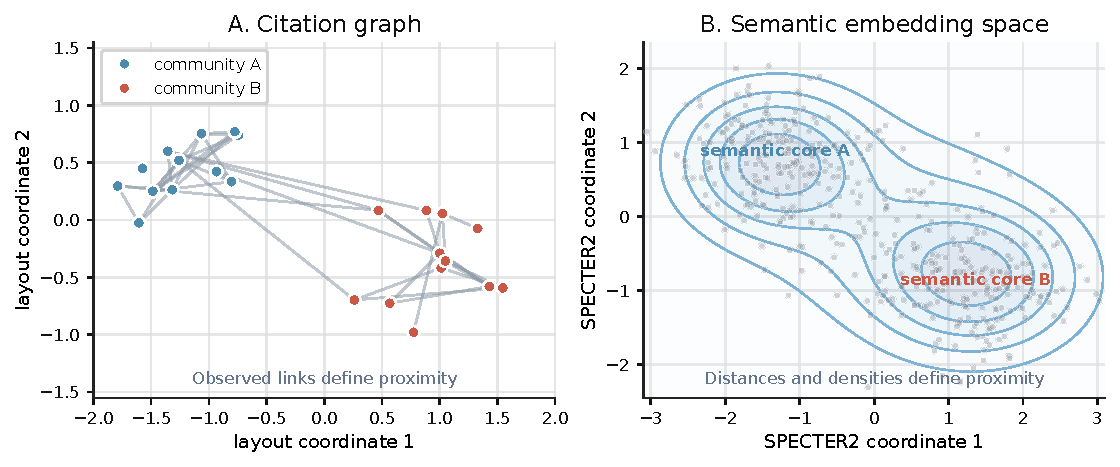
\includegraphics[width=\textwidth]{figures/fig_02_citation_semantic_contrast.pdf}
\end{figure}

The data source also matters. This thesis uses OpenAlex because it provides an open bibliographic infrastructure with works, concepts, venues, authors, institutions, and hierarchical research areas \parencite{priem2022openalex}. Open data makes the corpus auditable, but it does not remove coverage limits. Large bibliographic databases vary by field, document type, language, and metadata completeness \parencite{martinmartin2021google}, and recent comparisons document both the strengths of OpenAlex reference coverage and remaining metadata limitations \parencite{culbert2025reference}. For that reason, OpenAlex subfields are used as pragmatic analytical units, not as natural boundaries of science.

\section{Scientific Document Embeddings}

Scientific text is not generic text. Titles and abstracts contain specialized terminology, compressed argumentative structures, domain conventions, and technical phrases whose meaning depends on scientific context. Domain-adapted language models such as SciBERT were developed because scientific corpora differ systematically from general language corpora \parencite{beltagy2019scibert}. For this thesis, the relevant unit is not a word or sentence but a scientific work represented through its title and abstract.

SPECTER introduced document-level scientific embeddings learned with citation-informed supervision: papers that cite or are cited by one another provide a signal for document relatedness, so textual representation is trained with structural scholarly information \parencite{cohan2020specter}. SPECTER2 extends this line of work within the SciRepEval framework for evaluating scientific document representations across multiple task formats \parencite{singh2023scirepeval}. This makes SPECTER2 appropriate for a thesis that compares scientific works as documents rather than estimating word frequencies or topic mixtures.

The use of SPECTER2 does not mean that the embedding space is treated as ground truth. A 768-dimensional document vector is a compressed representation of title--abstract text under a particular model. It cannot capture the full methods, evidence, institutional context, or epistemic commitments of a paper. It can, however, provide a shared scientific document geometry in which sets of papers can be compared consistently. Chapter 4 explains the implemented representation pipeline; the role of the literature here is to justify why document-level scientific embeddings are a reasonable substrate for field-level morphology.

\section{From Semantic Location to Morphology}

Most uses of document embeddings begin with location: where is a paper, a topic, or a field in semantic space? Location is important, but it is incomplete. A centroid can summarize the average position of a field, yet it discards the field's internal spread, local packing, hub concentration, spectral structure, and temporal movement. The same field can be close in citation space, far in semantic location, and similar in morphology to another field. This thesis therefore shifts attention from where a field is located to how its papers occupy space around that location.

The idea has roots in earlier work on diversity, distance, and novelty. Stirling's diversity framework distinguishes variety, balance, and disparity, making clear that a collection cannot be characterized only by counting its elements \parencite{stirling2007diversity}. Work on cognitive distance similarly treats proximity and distance as conditions that shape learning and recombination \parencite{nooteboom2007cognitive}. Studies of scientific novelty show that unusual combinations can matter because they bridge distant regions of existing knowledge \parencite{uzzi2013atypical}. This thesis does not reproduce those measures directly. It adapts their intuition to dense semantic geometry: fields are distributions, and their shape can be measured.

Embedding-space morphology is the operational form of that idea. Dispersion describes how far papers spread around the field centroid. Local density describes how tightly papers pack into neighborhoods. Hubness describes whether a small subset of papers becomes disproportionately central in nearest-neighbor relations, a known phenomenon in high-dimensional spaces \parencite{radovanovic2010hubness}. Spectral structure summarizes how many principal directions are needed to describe variation. Temporal movement asks how those structures change across publication windows.

This geometric view requires caution. High-dimensional distances are affected by anisotropy, distance concentration, density variation, and hubness. Low-dimensional projections introduce a second layer of distortion. UMAP is a useful visualization method \parencite{mcinnes2018umap}, but nonlinear projections can change apparent distances, densities, and cluster shapes \parencite{chari2023specious,wattenberg2016tsne}. For that reason, this thesis uses PCA, PCoA, and UMAP only for communication and exploratory display. Quantitative morphology is computed in the original SPECTER2 embedding space.

\section{Positioning of This Thesis}

The gap addressed by this thesis lies between science mapping and scientific document representation. Existing science maps often emphasize bibliometric topology, classification overlays, topic structure, or two-dimensional visualization. Scientific document embeddings make a shared semantic geometry available, but they are often used to cluster papers, retrieve similar documents, or draw maps. Here the geometry is used differently: to measure field-level morphology.

The contribution is a disciplined separation of location, shape, trajectory, and taxonomy. Semantic location refers to where a subfield's centroid sits in embedding space. Static morphology describes the full-period shape of the subfield's paper distribution. Temporal trajectories describe how morphology changes across windows. Morphological similarity compares fields or subfields through profile distances. Clustering compresses those profiles into typological anchors, while remaining exploratory rather than taxonomic. This caution is important because no clustering procedure provides a uniquely objective partition of a data space \parencite{kleinberg2002clustering}.

This positioning narrows the claim. The thesis is not a topic model, a citation-network clustering project, a paper-level community detection study, a productivity or impact analysis, a UMAP-based map, or a replacement for OpenAlex taxonomy. Those approaches answer different questions. The present framework asks how field-level paper distributions are shaped in a shared scientific document geometry.

The following chapters make that question operational. Chapter 3 defines the OpenAlex corpus and the subfield as the analytical unit. Chapter 4 defines the SPECTER2 representation and the separation between measurement space and visualization. Chapter 5 develops the embedding-space morphology metrics. Chapters 6 to 9 then use those metrics to compare static morphology, temporal trajectories, morphological similarity, and exploratory typological structure.


\chapter{Data and Corpus Construction}
% Chapter 3: Data and Corpus Construction
% Focus: OpenAlex taxonomy, filtering rules, sampling design, and database validation diagnostics.
% Document Feeds: docs/data_corpus.md, docs/openalex_extraction_2000_2024_400py.md, docs/openalex_queries.md
% Outputs: outputs/01_corpus_construction/
% TODO: Add final corpus counts, fields, subfields, and domain distribution tables.
% TODO: Reference the specific 2000-2024 period and 400 papers/year/subfield sampling strategy.

\noindent This chapter describes the source data, corpus construction pipeline, and validation diagnostics. The corpus is extracted from OpenAlex using a rigorous sampling framework to ensure representativeness and statistical consistency across time and disciplines.

% TODO: Outline the hierarchical taxonomy of OpenAlex (Subfields, Fields, Domains).
% TODO: Detail sample extraction parameters: 2000-2024, 400 valid English title-plus-abstract records per year per subfield.
% TODO: Add table of overall corpus statistics (total documents, subfield coverage).
% TODO: Explain cleaning steps: filtering retracts, short abstracts, and non-supported document types.


\chapter{Semantic Representation}
% Chapter 4: Semantic Representation
% Focus: The SPECTER2 embedding architecture, embedding pipeline shards validation, and building the row-aligned analysis matrix.
% Document Feeds: docs/embedding_pipeline.md, docs/embed_specter2_kaggle.md
% Outputs: data/processed/analysis_embedding_index.parquet, main_embeddings.float16.npy
% TODO: Explain row alignment mapping (analysis_row_id to work_id).
% TODO: Provide mathematical description of how title + abstract text maps to 768-dimensional dense vector space.

\noindent This chapter details the technical and conceptual framework of document semantic representation. It documents the embedding pipeline, shard validation, and the row-aligned document matrix which serves as the quantitative foundation for all downstream morphological analyses.

% TODO: Detail SPECTER2 model selection, fine-tuning task adapters, and output vector space.
% TODO: Describe shard-by-shard embedding computation and the validation protocol.
% TODO: Define the mathematical mapping from text input to $\mathbb{R}^{768}$.
% TODO: Outline the contract between the embedding index and row-aligned matrices.


\chapter{Embedding-Space Morphological Metrics}
% Chapter 5: Embedding-Space Morphological Metrics

\section{From Embedded Papers to Morphological Indicators}

The previous chapter defined the semantic representation used in this thesis: a row-aligned matrix of SPECTER2 document embeddings linked to OpenAlex metadata. Chapter 5 turns that matrix into morphological indicators. The central move is to treat each subfield not only as a list of papers, but as a distribution of papers in a shared semantic geometry. A compact field and a fragmented field may contain the same number of papers; their difference lies in how those papers occupy embedding space.

Metric computation uses the original SPECTER2 coordinate system, with 768 dimensions. Non-zero vectors are L2-normalized, and distances are cosine distances. This fixes vector scale while preserving the original embedding dimensions; no UMAP projection or other low-dimensional map enters the quantitative metrics.

Let \(Z_s = \{z_i : i \in s\}\) denote the set of normalized embeddings for subfield \(s\), with \(n_s = |Z_s|\). The subfield centroid is

\[
c_s = \frac{1}{n_s}\sum_{i \in s} z_i.
\]

Distances to this centroid are computed as cosine distances to the centroid direction,

\[
r_i = d(z_i, c_s),
\]

where \(d(\cdot,\cdot)\) denotes cosine distance. The metrics below summarize the distribution of these distances, the structure of local neighborhoods, the spread of variance across principal directions, and temporal movement across the 2000--2024 period.

\section{Metric Families and Geometric Interpretation}

The reduced core contains eleven indicators organized into four families. The grouping is conceptual rather than decorative: each family answers a different morphological question. Dispersion asks how broad the semantic territory is. Local density and hubness ask how tightly papers are packed and whether some papers dominate neighborhood structure. Spectral structure asks whether variation is concentrated along a few directions or spread across many. Temporal movement asks whether the semantic position or radius of the subfield changes over time.

\begin{table}[H]
\centering
\caption{Reduced embedding-space metric core}
\label{tab:metric_core}
\scriptsize
\begin{tabular}{@{}>{\raggedright\arraybackslash}p{0.17\textwidth} >{\raggedright\arraybackslash}p{0.20\textwidth} >{\raggedright\arraybackslash}p{0.29\textwidth} >{\raggedright\arraybackslash}p{0.24\textwidth}@{}}
\hline
\textbf{Family} & \textbf{Metric} & \textbf{What it captures} & \textbf{High-value interpretation} \\
\hline
Semantic dispersion & Median centroid distance & Median distance from papers to the subfield centroid & Greater typical semantic dispersion \\
Semantic dispersion & Centroid-distance IQR & Interquartile range of centroid distances & More heterogeneous radial spread \\
Semantic dispersion & Centroid-distance P90 & 90th percentile of centroid distances & More distant semantic periphery \\
Local density & Median kNN distance & Median within-subfield nearest-neighbor distance & Lower local packing density \\
Local density & kNN distance CV & Coefficient of variation of kNN distances & More uneven local density \\
Hubness & kNN in-degree Gini & Gini coefficient of kNN in-degree counts & Stronger concentration around semantic hubs \\
Spectral structure & PCA dim80 & Components needed for 80 percent PCA variance & More distributed variance across directions \\
Spectral structure & PCA spectral entropy & Normalized entropy of the PCA variance spectrum & Flatter, less axis-dominated structure \\
Temporal movement & Centroid drift & Distance between early and late centroids & Greater net semantic movement \\
Temporal movement & Radial expansion slope & Trend in annual distance to the full-period centroid & Expansion away from the period center \\
Temporal movement & Recent novelty score & Late-period distance from the early semantic core & Recent papers farther from early structure \\
\hline
\end{tabular}
\par\vspace{0.2cm}
\footnotesize\textit{Note.} Metric names are shortened thesis labels. All metrics are computed on L2-normalized SPECTER2 embeddings in the original 768-dimensional space.
\end{table}


Together these metrics turn geometry into interpretable morphology. They do not assign a substantive label to a discipline, and they do not decide whether a field is intellectually better or worse. They describe how the papers in a subfield are arranged under a fixed representation model.

\section{Operational Definitions}

Semantic dispersion is measured from the centroid-distance distribution \(\{r_i : i \in s\}\). The median distance describes the typical radial position of papers around the subfield center. The interquartile range describes heterogeneity in the middle of the distribution. The 90th percentile captures the outer semantic periphery. A field can therefore be compact at the center while still having a long tail of distant papers.

Local density is computed from within-subfield nearest-neighbor distances. Let \(N_k(i)\) be the \(k\)-nearest-neighbor set of paper \(i\), with \(k = 15\) unless fewer non-self neighbors are available. The median kNN distance measures typical local packing; smaller values indicate tighter neighborhoods. The coefficient of variation of all directed kNN distances measures unevenness in local density. To capture hubness, each paper receives an in-degree count

\[
h_j = \sum_{i \in s} \mathbf{1}\{j \in N_k(i)\}.
\]

The metric \(\texttt{knn\_indegree\_gini}\) is the Gini coefficient of these counts. High values indicate that a small subset of papers appears disproportionately often as nearest neighbors. This is a known issue in high-dimensional spaces, where certain points can become unusually frequent neighbors across many queries \parencite{radovanovic2010hubness}.

Spectral structure is measured with PCA on the normalized embeddings of each subfield. Let \(\lambda_1,\ldots,\lambda_p\) be the PCA explained-variance values, with \(p \leq 768\) depending on the number of available observations and positive-variance components. The 80 percent dimensionality proxy is

\[
D_{80}(s) = \min \left\{m : \frac{\sum_{j=1}^{m} \lambda_j}{\sum_{j=1}^{p} \lambda_j} \geq 0.80 \right\}.
\]

Higher values mean that more principal components are needed to explain the same share of variance. This is an operational PCA proxy, not a claim about the true intrinsic dimension of a field.

The spectral entropy metric summarizes how evenly variance is distributed across PCA directions:

\[
H(s) = -\frac{\sum_{j=1}^{q} p_j \log p_j}{\log q},
\qquad
p_j = \frac{\lambda_j}{\sum_{\ell=1}^{q} \lambda_\ell},
\]

where \(q\) is the number of positive-variance components. Values are normalized by \(\log q\), so higher entropy indicates a flatter variance spectrum and less dominance by a few directions.

Temporal morphology is measured with three indicators. The first, \(\texttt{centroid\_drift}\), is the cosine distance between the centroid of the early period and the centroid of the late period. For the full thesis window, the early period is 2000--2004 and the late period is 2020--2024:

\[
\Delta_c(s) = d(c_s^{early}, c_s^{late}).
\]

The second, \(\texttt{radial\_expansion\_slope}\), is the linear slope of annual median distance to the full-period centroid. If \(a_{s,t}\) is the median distance of papers published in year \(t\) to \(c_s\), then the metric is the fitted slope \(\hat{\beta}_1\) in

\[
a_{s,t} = \beta_0 + \beta_1(t-\bar{t}) + \varepsilon_t.
\]

Positive values indicate expansion away from the period centroid; negative values indicate contraction toward it. The third temporal metric, \(\texttt{recent\_novelty\_score}\), compares late papers with the early semantic core:

\[
R(s) =
\operatorname{median}_{i \in late} d(z_i, c_s^{early})
-
\operatorname{median}_{i \in early} d(z_i, c_s^{early}).
\]

A positive value means that recent papers are farther from the early-period centroid than early papers were. These temporal metrics describe movement and radial change; they do not identify causes.

\section{Reduction to an Interpretable Metric Core}

The full metric computation produces more diagnostic quantities than are used in the main thesis analysis. The reduced core keeps eleven indicators because they cover four distinct aspects of morphology while avoiding a long list of near-duplicate summaries. The aim is not to maximize the number of features, but to preserve interpretability across subfields.

The retained dispersion metrics describe the global radius of a subfield. The retained kNN metrics describe local packing and hub concentration. The retained PCA metrics describe spectral complexity. The retained temporal metrics describe movement, expansion, and recent departure from earlier structure. Other computed quantities are useful for diagnostics and sensitivity checks, but they are not part of the main morphological profile.

This reduction also protects the empirical chapters from false precision. A larger metric inventory can make results appear richer while mostly repeating the same information. The eleven-metric core is deliberately small enough to interpret and broad enough to distinguish compactness, heterogeneity, dimensionality, and temporal change.

\section{Interpretation and Limits of the Metrics}

Metric values are comparative. A high centroid-distance median indicates greater semantic dispersion relative to other subfields measured in the same embedding geometry. A high kNN median distance indicates sparse local neighborhoods. A high kNN in-degree Gini indicates concentration of neighborhood attention around a smaller set of papers. A high \(D_{80}\) or spectral entropy indicates that variation is spread across more directions. Positive radial expansion and recent novelty indicate movement away from earlier or full-period semantic structure.

These interpretations remain conditional on the corpus and representation. The metrics do not measure field size, publication volume, citation impact, research quality, or institutional importance. They also do not reveal the essence of a discipline. They describe reproducible structure in a model-defined semantic space.

Dimensionality reduction is not part of the metric system. UMAP maps may help visualize scientific space, but the indicators in this chapter are computed from the original SPECTER2 vectors. The empirical chapters therefore use low-dimensional plots as illustrations, not as evidence for metric distances, density, or movement.


\chapter{Static Comparison of Scientific Disciplines}
% Chapter 4: Static Morphology Across Scientific Fields

\section{Exploratory Metric Diagnostics}

Before comparing fields, I inspect the raw distributions of the eight structural metrics. Their shapes differ clearly. Centroid-distance IQR is right-skewed, kNN distance CV has a visible upper tail, and PCA D80 is partly discrete. The remaining metrics are more symmetric, although they also contain a small number of extreme values. These differences support the use of median/IQR scaling. This makes metrics with different ranges comparable and prevents a few extreme subfields from determining the scale, while keeping those unusual cases visible in the analysis.

\begin{figure}[H]
\centering
\caption[Raw structural metric distributions]{Raw subfield distributions of the eight structural morphology metrics. Dashed vertical lines mark medians.}
\label{fig:structural_metric_raw_distributions}
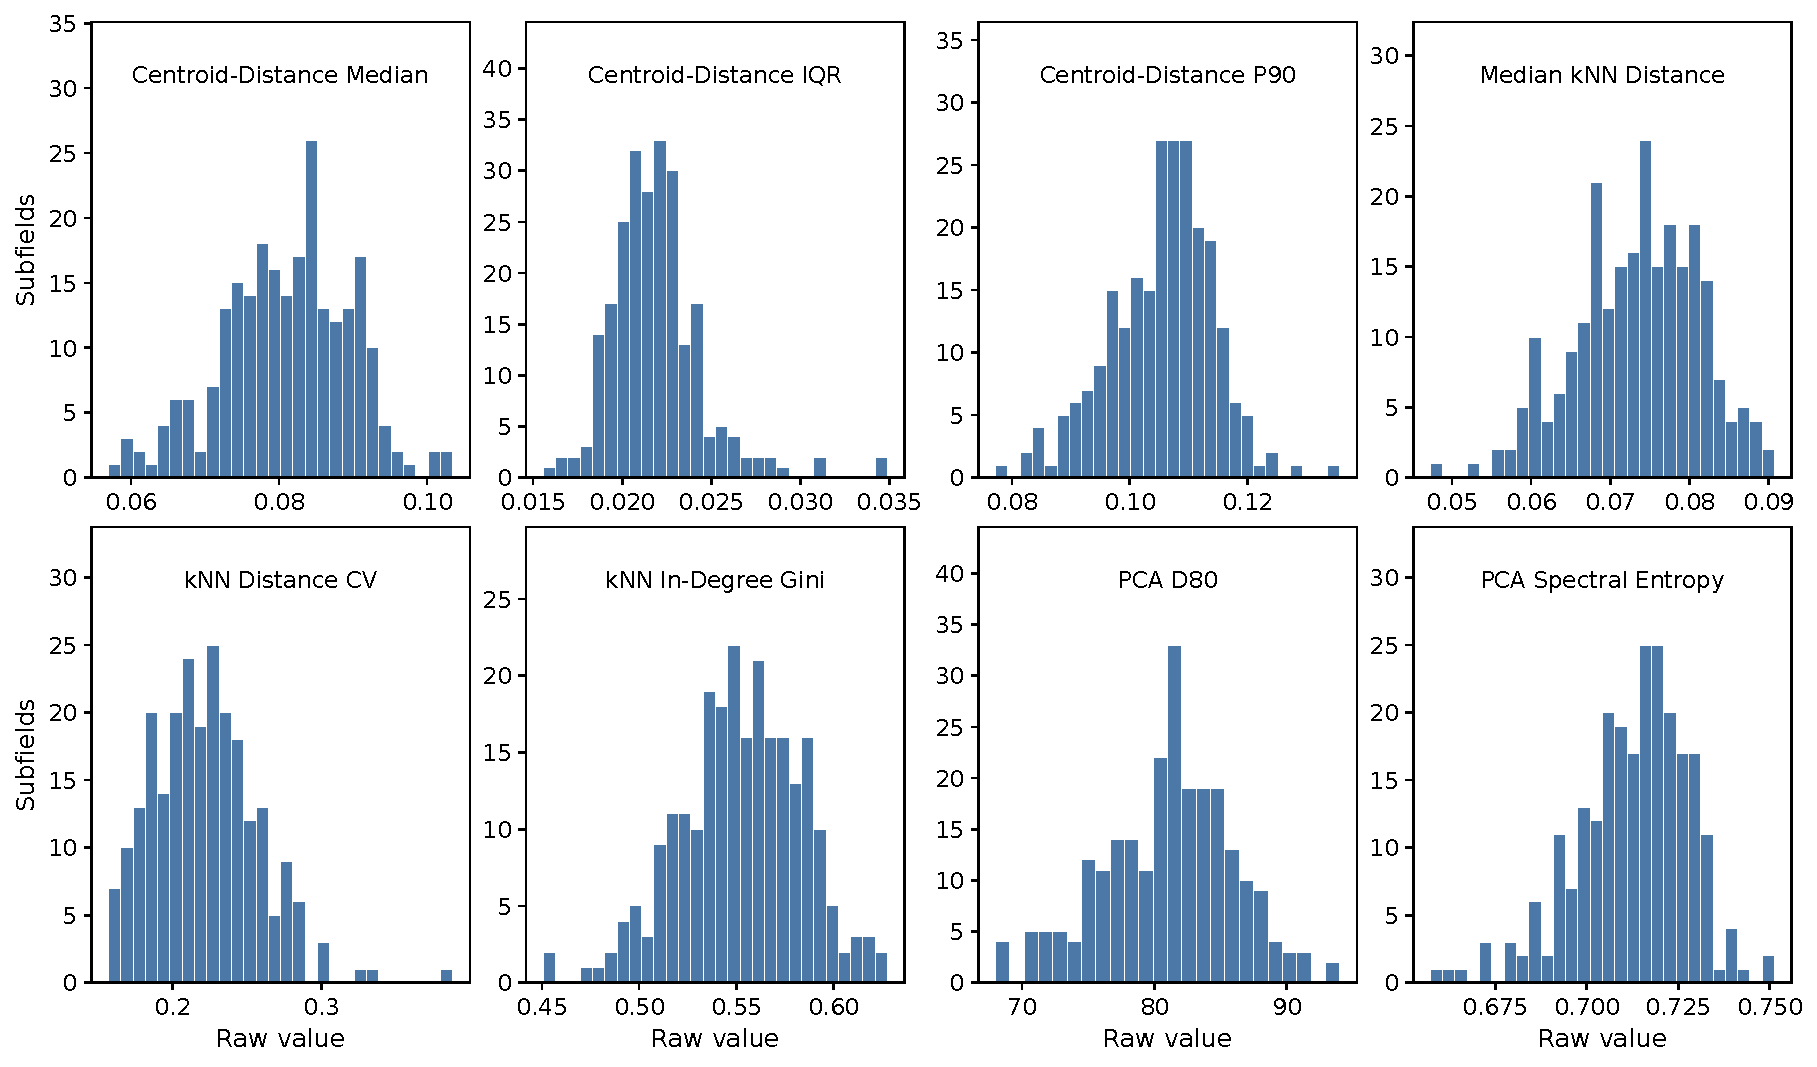
\includegraphics[width=\textwidth]{figures/fig_06_structural_metric_raw_distributions.pdf}
\end{figure}

The correlations show that some metrics are related, but the families are not redundant. Centroid median and centroid P90 are strongly correlated (\(\rho=0.883\)), as expected for two measures of radial spread. PCA \(D_{80}\) and PCA entropy are also strongly related (\(\rho=0.856\)), because both summarize the variance spectrum. The largest negative relation is between kNN median distance and kNN CV (\(\rho=-0.798\)): subfields with closer local neighborhoods often have more uneven local packing. Correlations across different families are weaker. This supports keeping global dispersion, local density, hubness, and spectral structure as separate dimensions.

\begin{figure}[H]
\centering
\caption[Structural metric Spearman correlations]{Spearman correlation matrix for the eight raw structural morphology metrics.}
\label{fig:structural_metric_spearman_correlation}
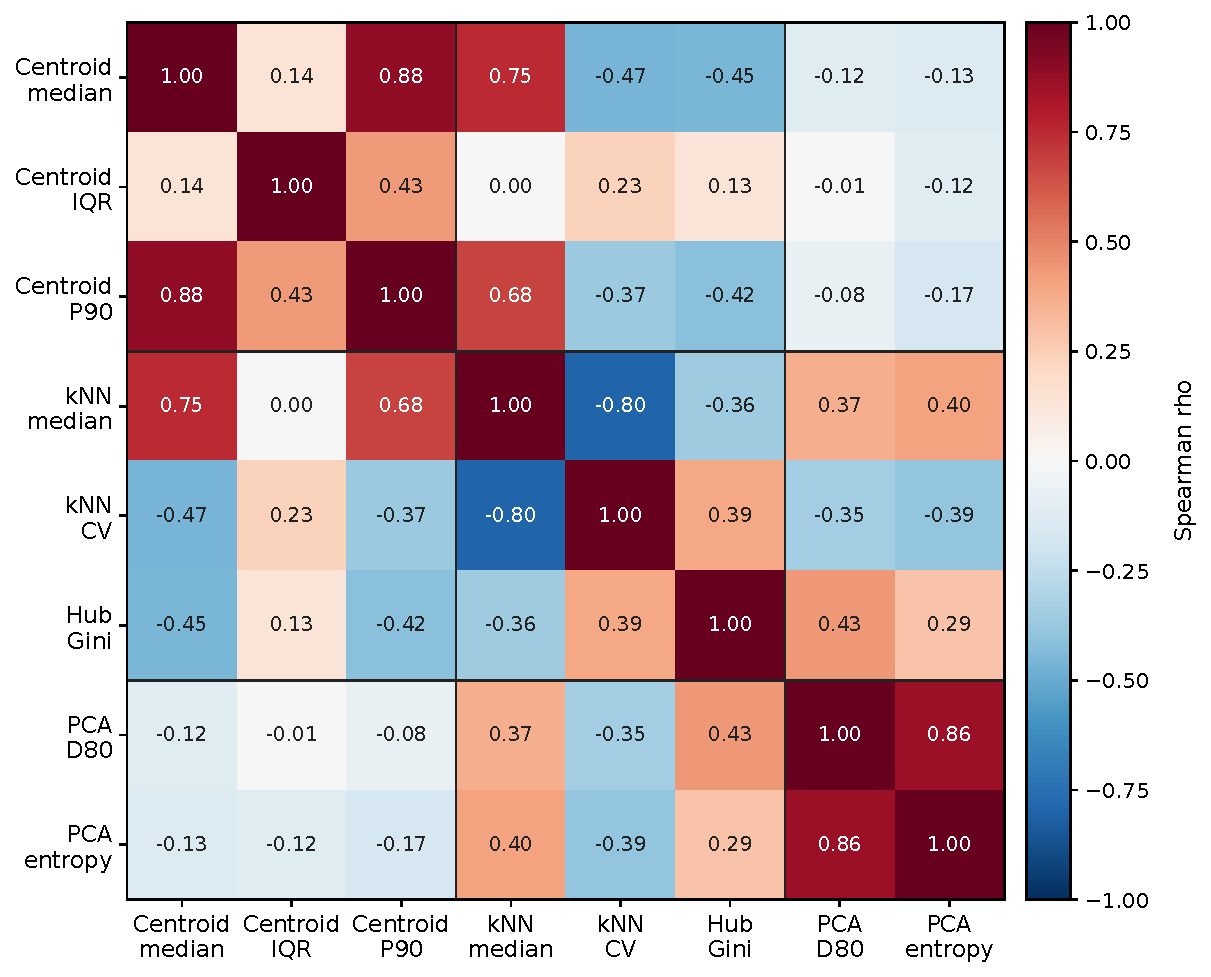
\includegraphics[width=0.78\textwidth]{figures/fig_06_structural_metric_spearman_correlation.pdf}
\end{figure}

\section{Domain Tendencies}

Static comparison uses one full-period structural morphology profile for each subfield. These profiles use the eight metrics defined in Chapter 3. Subfields are the direct measurement units; field and domain profiles are averages of standardized subfield profiles. In the heatmaps and boxplots, red indicates values above the median for that metric and blue indicates values below the median.

At the broadest scale, domains show tendencies. Physical Sciences are generally more dispersed and more spectrally extended. Health Sciences show tighter local neighborhoods and stronger local concentration. Social Sciences and Life Sciences are closer to the center of most metrics, with specific departures rather than one clear profile.

One possible interpretation is that Physical Sciences contain several well-developed research directions that use different concepts, methods, and technical languages. This could produce a document cloud with several broad directions rather than one compact centre. In Health Sciences, research may be organized more often around recurring diseases, treatments, clinical procedures, or highly connected reference topics. This could explain why papers form tighter local groups and why some papers occupy more central positions in the neighbourhood structure. The weaker domain-level patterns in Life Sciences and Social Sciences may reflect a mixture of very different fields whose profiles partly cancel out when they are averaged. These interpretations are plausible, but the metrics alone cannot identify the scientific causes behind the observed shapes.

\begin{figure}[H]
\centering
\caption[Domain-level morphological profiles]{Domain-level standardized structural morphology profiles. Values are visual contrasts across the four domain profiles, not inferential statistics.}
\label{fig:domain_metric_profile_heatmap}
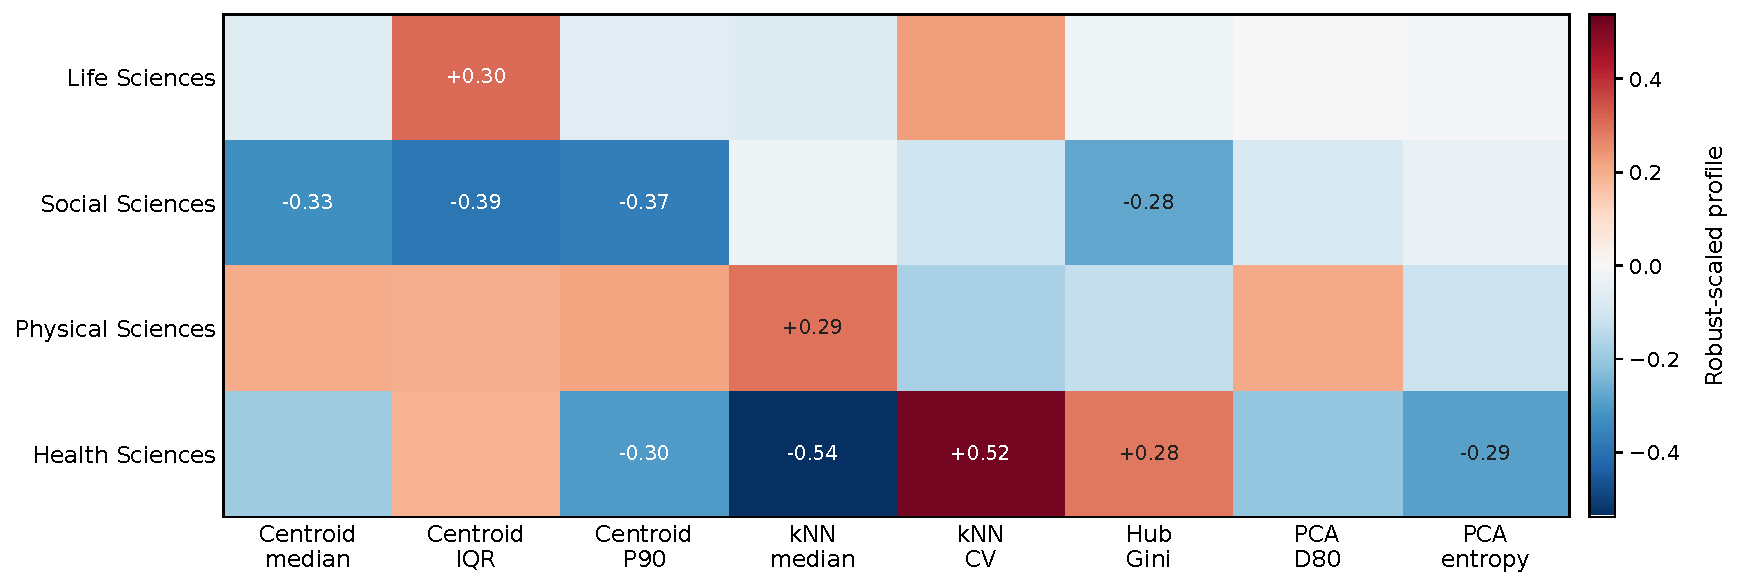
\includegraphics[width=\textwidth]{figures/fig_06_domain_metric_profile_heatmap.pdf}
\end{figure}

The domain view gives the first answer to the static part of the second research question: broad areas of science differ in shape. It is only a first answer. Four domain averages can hide strong variation among fields and subfields.

\section{Field and Subfield Heterogeneity}

Field profiles make the domain pattern less simple. Physical Sciences include dispersed fields such as Physics and Astronomy, Computer Science, Engineering, and Environmental Science. They also include more compact fields such as Energy and Mathematics. Health Sciences include dense fields such as Dentistry and Nursing, while Medicine sits closer to the center of the field distribution. Domains therefore show tendencies, not uniform morphologies.

The field-level profiles also show that fields can be unusual in different ways. Computer Science and Physics and Astronomy stand out mainly because their papers are spread more widely around the field centre. Chemistry, Materials Science, Engineering, and Environmental Science show larger distances between neighbouring papers, suggesting looser or more separated local research regions. Dentistry and Nursing show the opposite local pattern: their papers form tighter neighbourhoods, which may reflect research organized around recurring clinical problems, procedures, or treatments. Energy and Mathematics are important counterexamples within Physical Sciences because their more compact profiles differ from the broad pattern of their parent domain. Medicine remains closer to the middle of the field distribution, so the average Health Sciences profile is more strongly influenced by fields such as Dentistry, Nursing, and Health Professions. Figure 4.4 therefore helps distinguish whether a domain tendency is widely shared, driven by a few fields, or produced by opposite field profiles that partly cancel out when averaged.

\begin{figure}[H]
\centering
\caption[Field-level morphological profiles]{Field-level standardized structural morphology profiles. Rows are fields ordered by parent OpenAlex domain.}
\label{fig:field_metric_profile_heatmap}
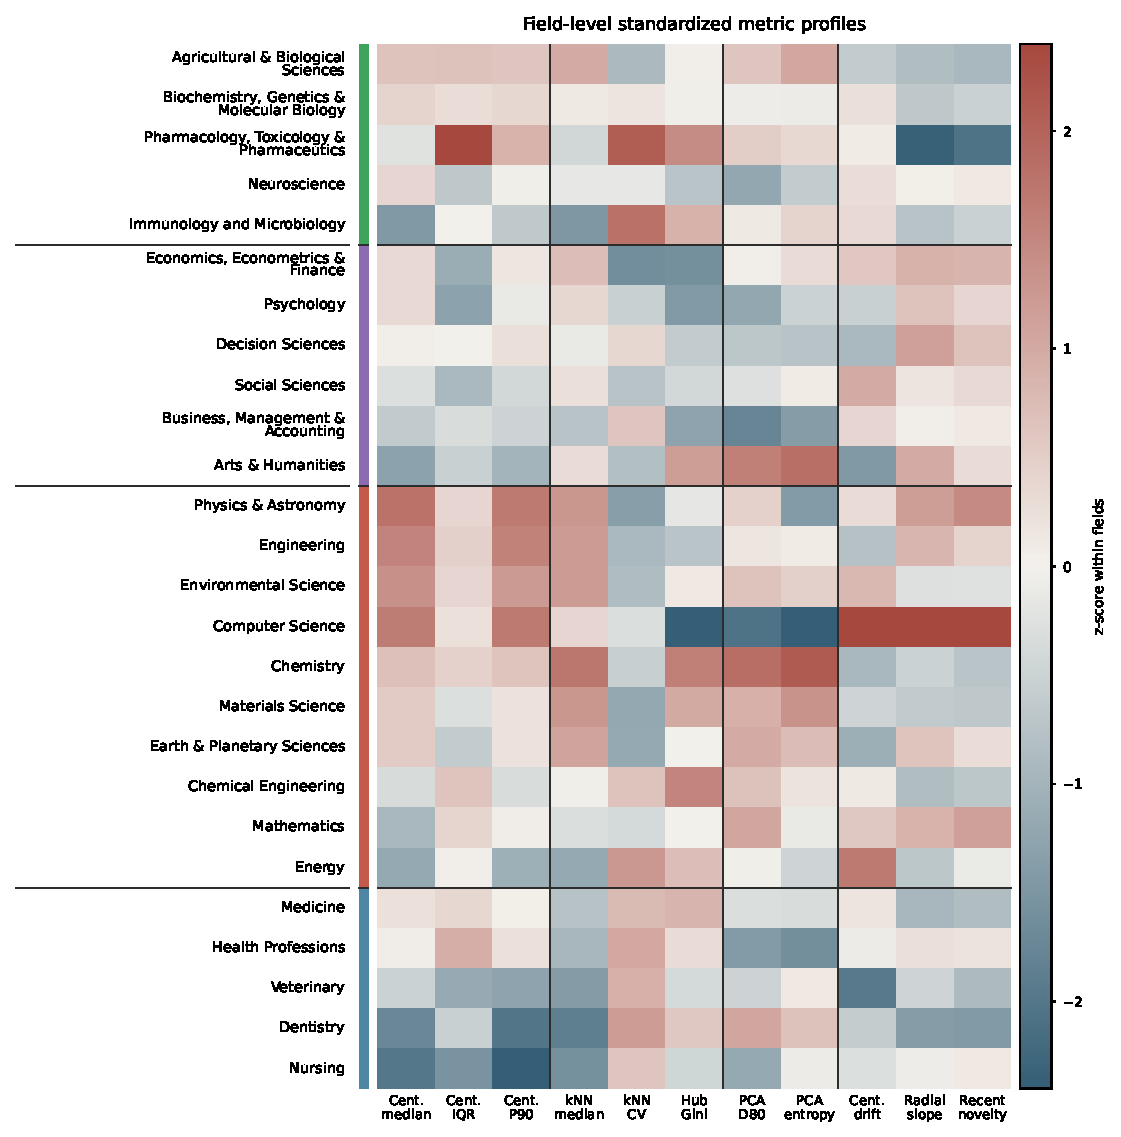
\includegraphics[width=\textwidth,height=0.78\textheight,keepaspectratio]{figures/fig_06_field_metric_profile_heatmap.pdf}
\end{figure}

The heatmap also reveals combinations that are hidden by a simple broad-versus-compact comparison. Computer Science has a wide overall spread, but low hubness and low spectral values, meaning that its variation is concentrated in fewer main directions and is not organized around a small set of dominant neighbouring papers. Arts and Humanities shows almost the opposite profile: it is relatively compact around its centre, but has higher hubness and spectral complexity. Pharmacology, Toxicology and Pharmaceutics stands out for a different reason, with very uneven distances both from the centre and within local neighbourhoods. These cases show that overall spread, local organization, hub concentration, and spectral structure can change independently. Two fields with a similar radius can therefore have very different internal structures.

\begin{figure}[H]
\centering
\caption[Subfield metric distributions by domain]{Subfield-level standardized metric distributions by domain for the eight structural metrics.}
\label{fig:subfield_metric_distributions_by_domain}
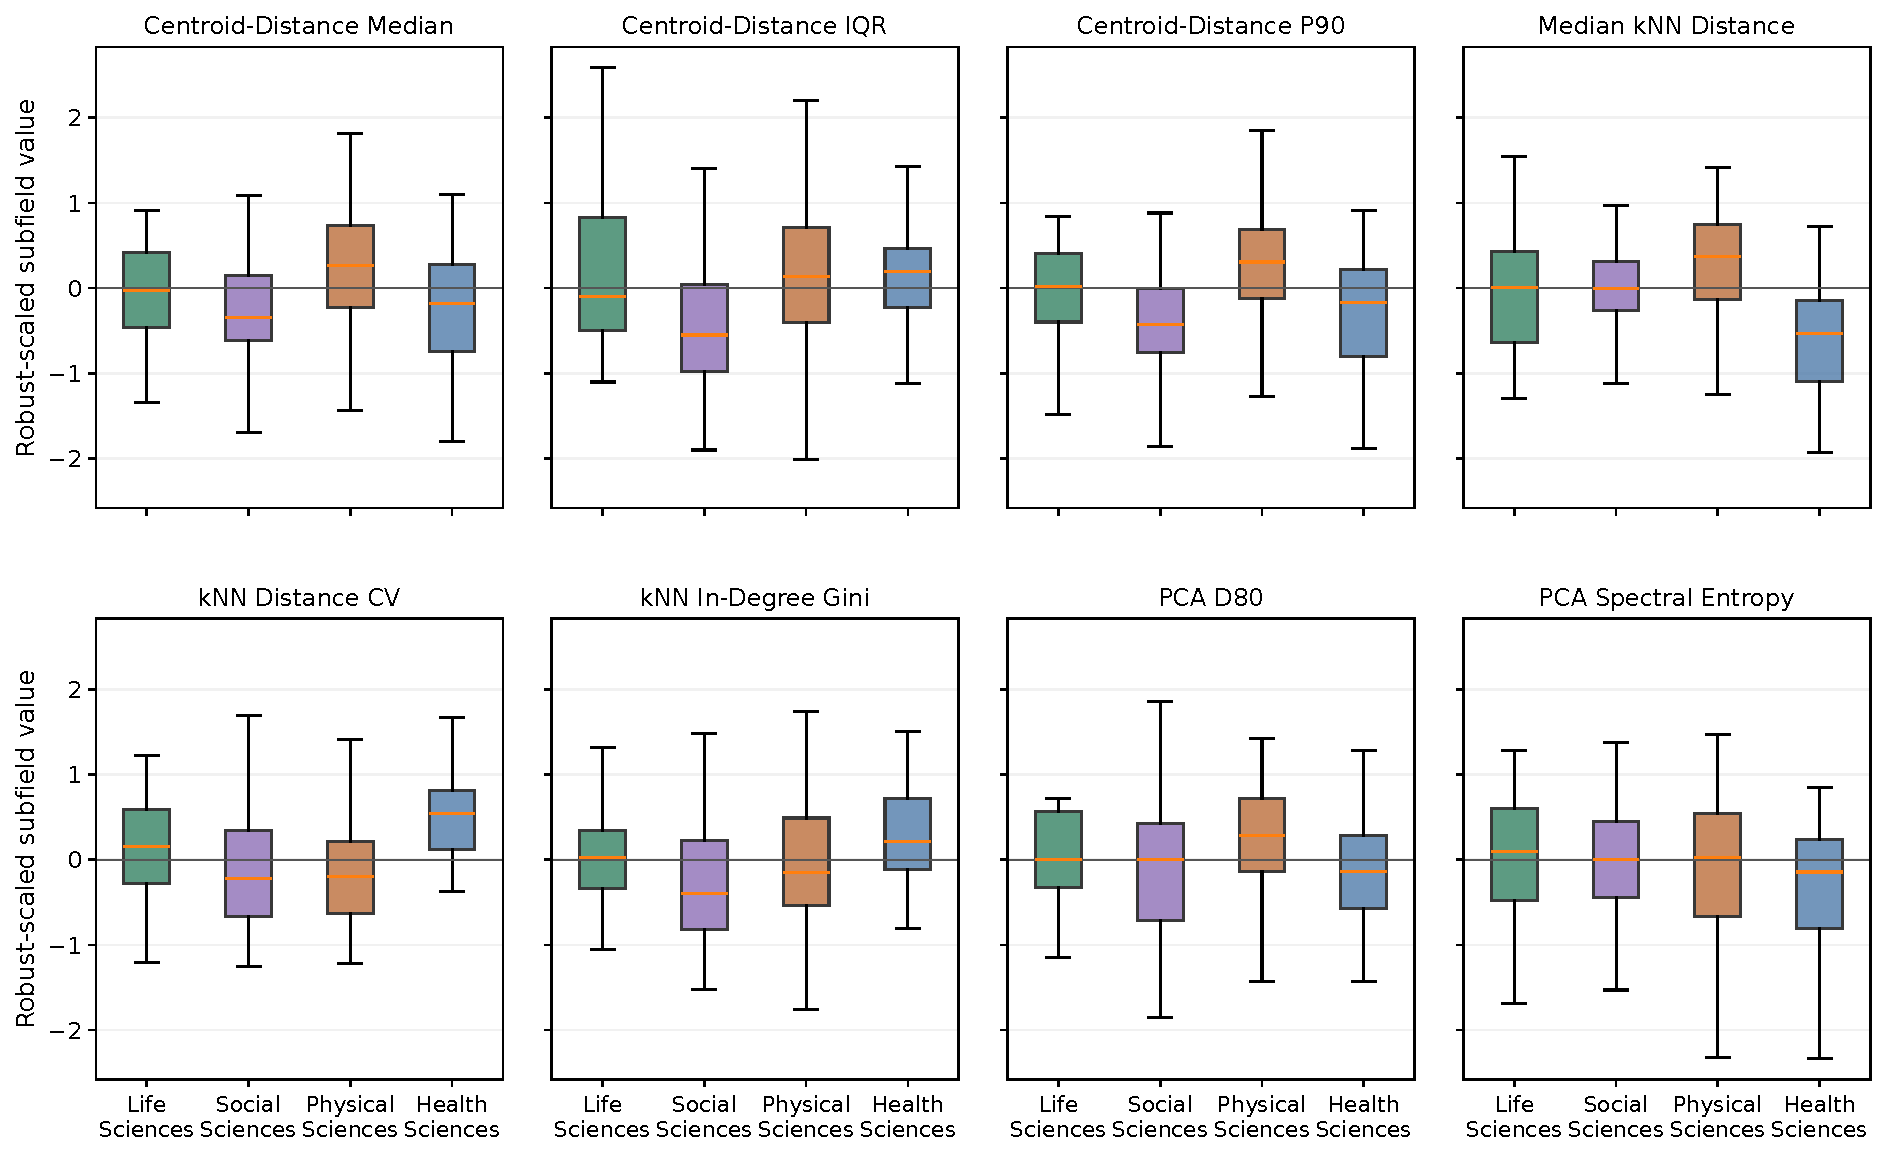
\includegraphics[width=\textwidth]{figures/fig_06_subfield_metric_distributions_by_domain.pdf}
\end{figure}

The boxplots show why morphology cannot be inferred from a domain label alone. Physical Sciences have the highest median subfield dispersion and kNN distance, but some physical subfields are compact. Health Sciences have lower local distances on average, but hubness varies widely. Social Sciences contain both compact applied areas and atypical humanities subfields. Field and subfield profiles are therefore not minor details after the domain result. They show where taxonomy and morphology partly separate.

\section{Metric Extremes and Profile Space}

Selected extremes make the same point with auditable cases. Nuclear and High Energy Physics and Artificial Intelligence sit at the high end of median centroid distance, while Applied Microbiology and Biotechnology and General Energy sit at the compact end. Molecular Medicine and Philosophy have unusually high centroid-distance IQR; Research and Theory and Algebra and Number Theory sit at the opposite end. Other metric families cut across these dispersion patterns. A field can be broad without being hub-dominated, and a compact field can still be locally uneven.

The standardized values in Table 4.1 show how unusual each subfield is relative to the rest of the sample. A value close to zero means that the subfield is near the median for that metric. Positive values indicate higher values and negative values indicate lower values. Because the scale is based on the median and the interquartile range, a score of +2 means two interquartile ranges above the median; it does not mean that the raw metric is twice as large. This also explains why some metrics can produce very large standardized scores even when their raw numerical range is small.

\begin{table}[H]
\centering
\caption{Selected subfield extremes in the static metric profiles}
\label{tab:extreme_subfields}
\scriptsize
\begingroup
\setlength{\tabcolsep}{2pt}
\begin{tabular}{@{}>{\raggedright\arraybackslash}p{0.17\textwidth} >{\raggedright\arraybackslash}p{0.25\textwidth} >{\raggedright\arraybackslash}p{0.25\textwidth} >{\raggedright\arraybackslash}p{0.21\textwidth}@{}}
\hline
\textbf{Metric} & \textbf{High end} & \textbf{Low end} & \textbf{Interpretation} \\
\hline
Median Centroid Distance & Nuclear and High Energy Physics; Artificial Intelligence; Electrical and Electronic Engineering & Applied Microbiology and Biotechnology; General Energy; Research and Theory & Broadest versus most compact semantic territories. \\
Median kNN Distance & Molecular Biology; Materials Chemistry; Biomedical Engineering & Applied Microbiology and Biotechnology; Internal Medicine; General Energy & Sparsest versus tightest local neighborhoods. \\
kNN In-Degree Gini & General Materials Science; Electrochemistry; Internal Medicine & Artificial Intelligence; Computer Vision and Pattern Recognition; Cognitive Neuroscience & Most versus least hub-concentrated neighborhood structure. \\
PCA D80 & Classics; Religious studies; Electrochemistry & Business and International Management; Computational Mathematics; Human Factors and Ergonomics & Most versus least distributed PCA variance. \\
Recent Novelty Score & Computer Vision and Pattern Recognition; Signal Processing; Human Factors and Ergonomics & Pharmaceutical Science; Molecular Medicine; Animal Science and Zoology & Recent work farthest from versus closest to the early semantic core. \\
\hline
\end{tabular}
\endgroup
\par\vspace{0.15cm}
\footnotesize\textit{Note.} Extremes are computed on raw metric values among the 241 eligible subfields; table entries list the top three subfields at each end of the selected metric.
\end{table}


These cases are not simply the largest or most productive subfields. Because the corpus is balanced, they appear in the table because the arrangement of their papers is unusual for a specific metric. The differences therefore reflect structure in the embedding space rather than publication volume.

The extremes also show why a single composite score would lose information. Human Factors and Ergonomics is unusual in spectral entropy, Applied Microbiology and Biotechnology in local-density variability, Classics and Religious studies in spectral extension, and Artificial Intelligence in low hub concentration. These are different kinds of structure. Keeping the metric families separate preserves those differences.

The exploratory PCA map in Figure~\ref{fig:metric_profile_pca_map} summarizes standardized structural profiles, not paper-level semantic locations. The first two axes explain 35.9 percent and 31.8 percent of the standardized profile variance. Domains overlap near the center. The most informative cases are specific subfields at the edges of the profile space.

\begin{figure}[H]
\centering
\caption[Subfield profile PCA map]{Exploratory PCA map of subfield structural morphology profiles. Points are subfields represented by the eight standardized structural metrics.}
\label{fig:metric_profile_pca_map}
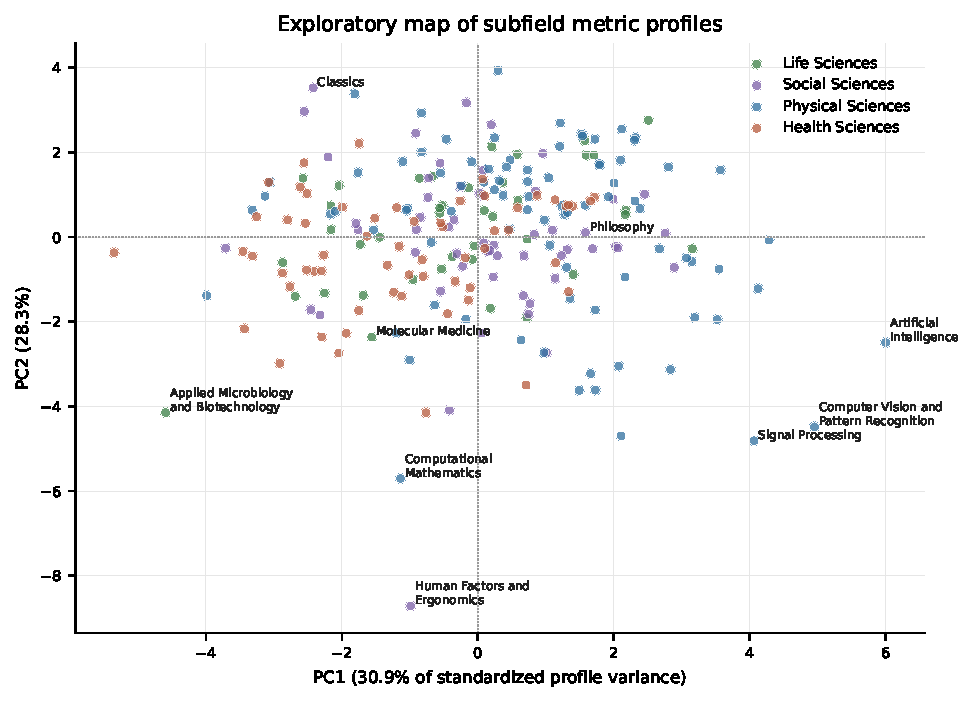
\includegraphics[width=\textwidth]{figures/fig_06_metric_profile_pca_map.pdf}
\end{figure}

The static result is clear but limited. Domains help orient the comparison, but they do not determine field shape. Broad domain tendencies coexist with large within-domain variation and cross-domain overlap in metric-profile space. Appendix~\ref{app:umap-atlas} keeps selected UMAP maps only as visual diagnostics. The next chapter therefore moves from full-period shape to structural change over time.


\chapter{Temporal Evolution of Scientific Morphology}
% Chapter 5: Temporal Evolution and Dynamic Profiles

\section{Temporal Trajectories of Structural Metrics}

Chapter 4 described the full-period morphology of fields and subfields. This chapter asks whether those profiles stay stable or change over time. I use five fixed windows: 2000--2004, 2005--2009, 2010--2014, 2015--2019, and 2020--2024. Within each window, I recompute the same eight structural metrics used in the static profile. This keeps the temporal analysis directly comparable with the static one.

Each subfield-window is treated as a separate document cloud. The windowed plots use robust-scaled values computed across all completed subfield-window observations. The temporal matrix is almost complete: 1,204 of 1,205 expected subfield-window rows were computed. Computational Mathematics in 2000--2004 is excluded only when a first--last comparison requires a complete trajectory.

The broad movement is toward closer local packing. Across all subfields, mean median centroid distance declines from 0.0858 in 2000--2004 to 0.0750 in 2020--2024. Mean median kNN distance declines from 0.0923 to 0.0756, and PCA \(D_{80}\) falls from 81.3 to 71.1. At the same time, kNN distance variability rises. This is not a simple contraction. The retained document clouds become closer locally on average, but the local spacing becomes less even.

These metrics describe different parts of the same movement. A lower centroid median means that papers are closer, on average, to the window centroid. A lower median kNN distance means that nearby papers are closer to each other. A lower PCA \(D_{80}\) means that fewer principal directions are needed to describe most of the variation. When kNN distance variability rises at the same time, the interpretation becomes more nuanced: some local neighborhoods tighten more than others. Figure~\ref{fig:domain_temporal_trajectories} should therefore be read as a set of related changes, not as eight independent trends.

\begin{figure}[H]
\centering
\caption[Domain-level temporal trajectories]{Domain-level temporal trajectories across five-year windows. Values are mean standardized subfield-window structural metrics within each domain.}
\label{fig:domain_temporal_trajectories}
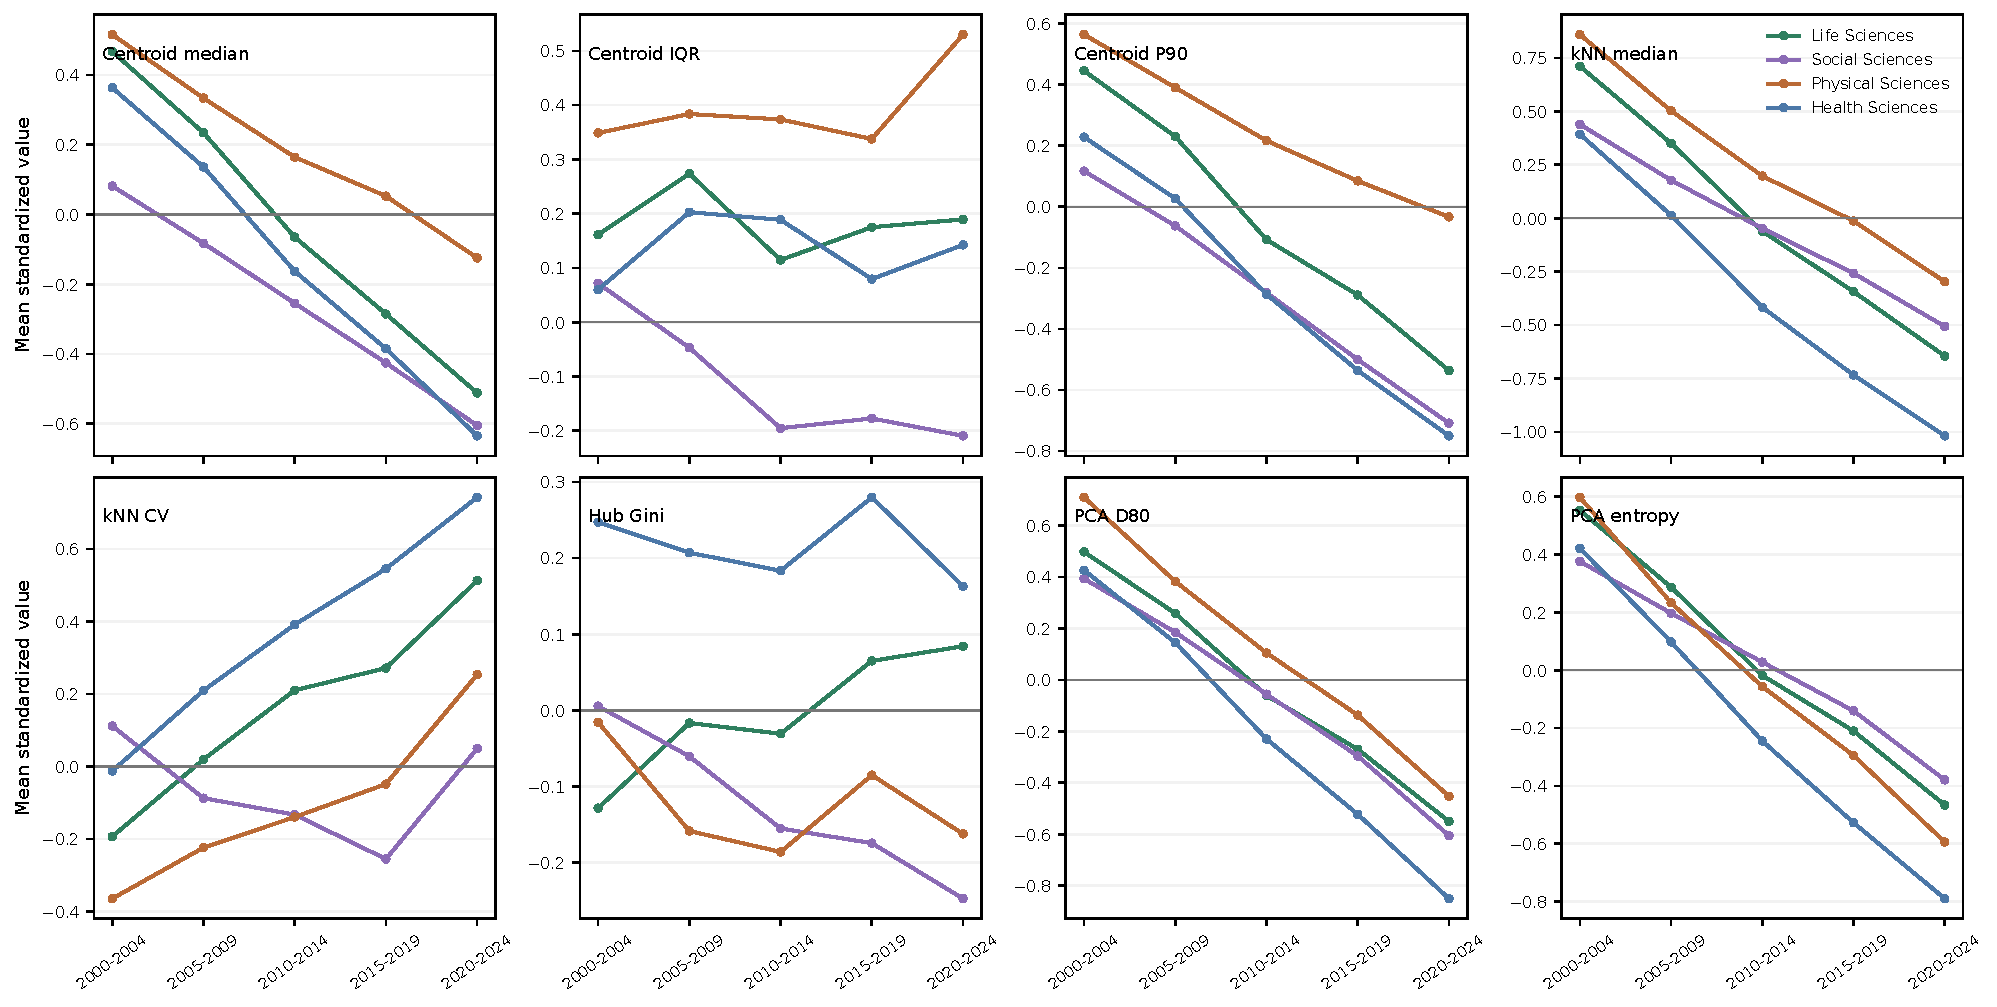
\includegraphics[width=\textwidth]{figures/fig_07_domain_temporal_trajectories.pdf}
\end{figure}

The domain trajectories give a first orientation. Physical Sciences remain the most dispersed domain for most of the period and keep the highest average spectral dimensionality. Health Sciences move furthest downward in local distance and PCA \(D_{80}\). They finish with the tightest local neighborhoods and the lowest average dimensionality. Life Sciences follow the same direction, with a clearer rise in kNN distance variability. Social Sciences are less extreme in the domain averages. As in the static chapter, this makes the field and subfield levels necessary.

\section{Fields and Subfields in Motion}

Field-level first--last deltas show where the average trajectory is strongest. The heatmap compares standardized field profiles in 2020--2024 with their profiles in 2000--2004. Negative values mean that the metric is lower at the end of the period, and positive values mean that it is higher. These changes should be read as changes in shape, not as improvement or decline.

Median centroid distance declines most clearly in Energy, Medicine, Dentistry, Chemical Engineering, and Pharmacology, Toxicology and Pharmaceutics. Median kNN distance declines most clearly in Dentistry, Energy, Medicine, Chemistry, and Immunology and Microbiology. Hubness does not follow the same direction. Energy and Immunology and Microbiology move upward in hub concentration, while Computer Science, Engineering, Psychology, and Health Professions move downward.

\begin{figure}[H]
\centering
\caption[Field-level temporal change heatmap]{Field-level temporal change from 2000--2004 to 2020--2024. Cells are final-minus-initial standardized structural values.}
\label{fig:field_temporal_delta_heatmap}
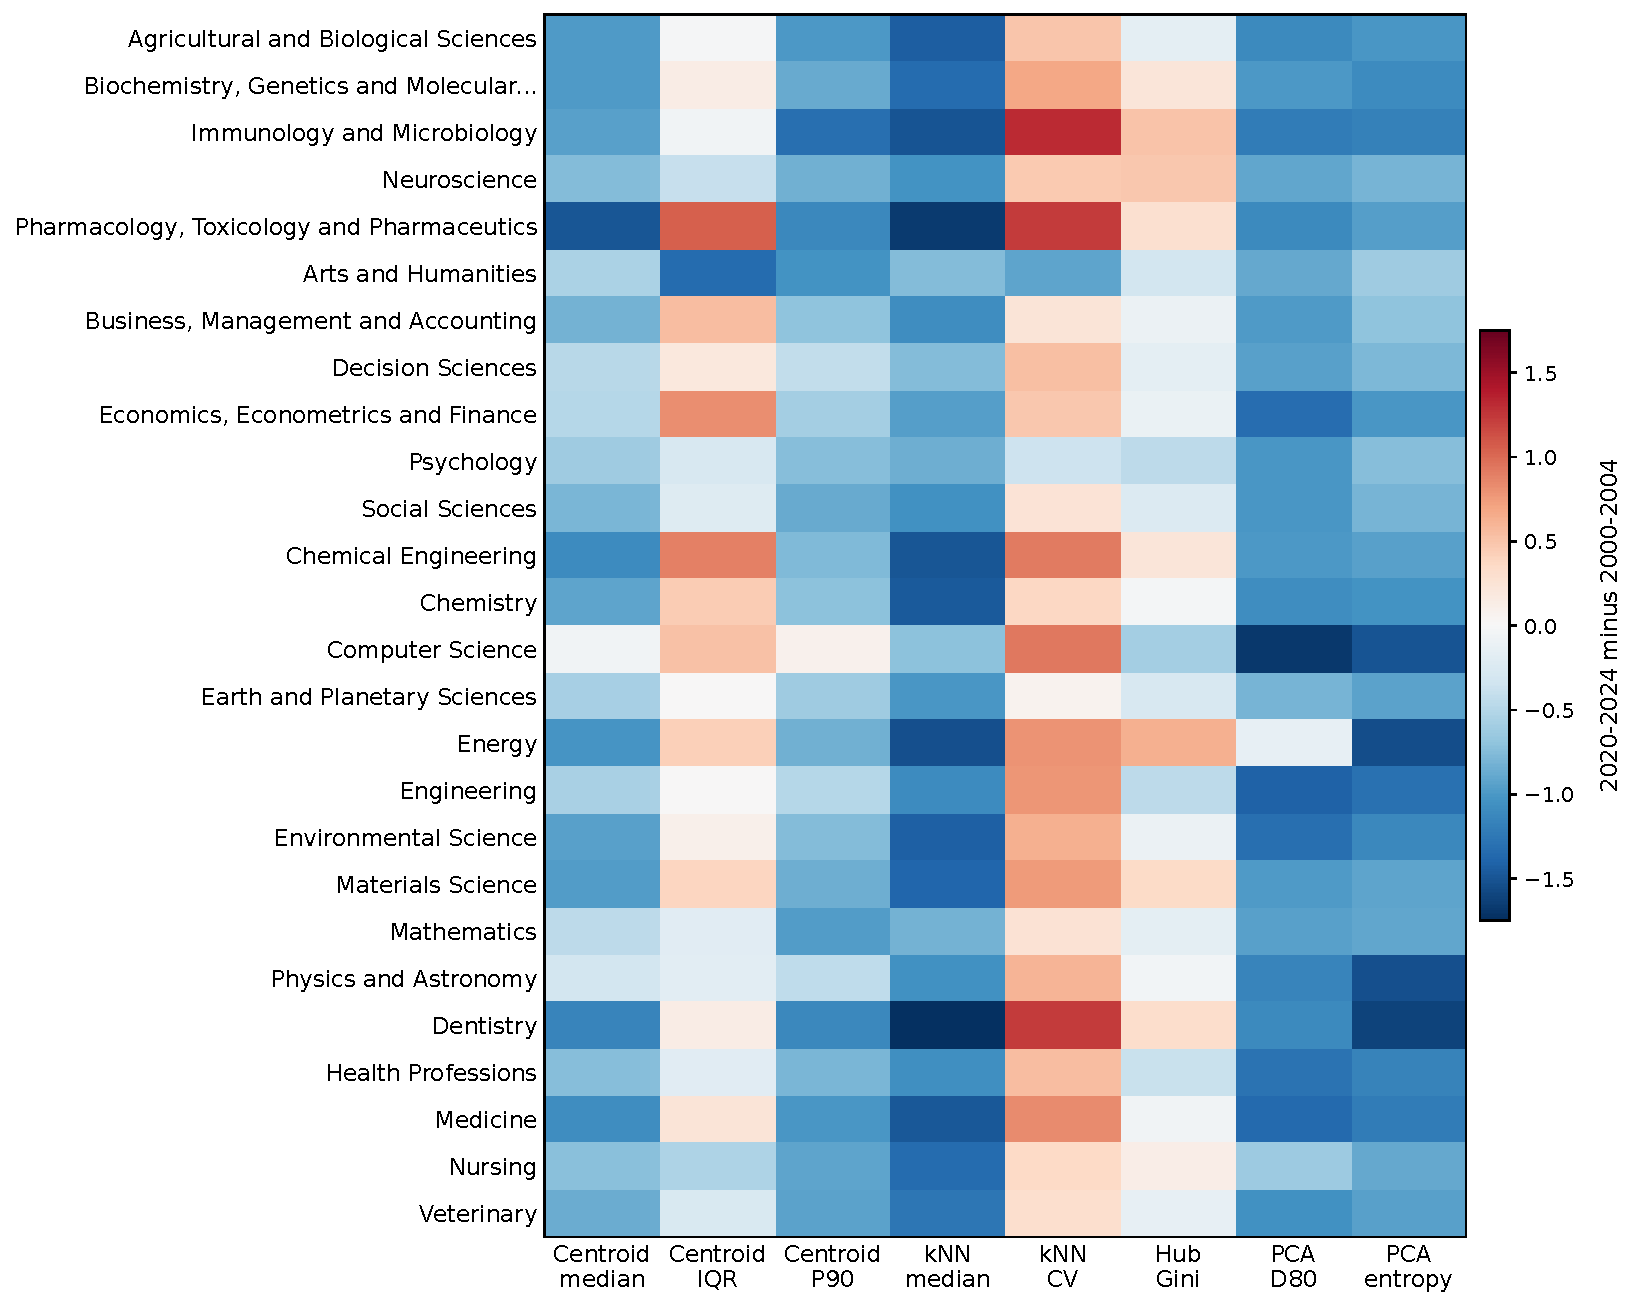
\includegraphics[width=\textwidth,height=0.80\textheight,keepaspectratio]{figures/fig_07_field_temporal_delta_heatmap.pdf}
\end{figure}

The field changes therefore do not describe one universal temporal direction. Some fields become more compact around their centroid or in their local neighborhoods. Other fields change mainly through hubness or spectral structure. This is why the temporal profile keeps the same eight metrics instead of reducing change to one expansion or contraction measure.

The strongest first--last profile changes are concentrated in a small set of subfields. Philosophy has the largest windowed structural displacement, followed by General Dentistry, Molecular Medicine, General Psychology, Immunology and Allergy, Infectious Diseases, Renewable Energy, Sustainability and the Environment, Pharmacy, Instrumentation, and Virology. The ranking measures Euclidean distance between initial and final standardized profiles across the eight windowed structural metrics.

\begin{figure}[H]
\centering
\caption[Most dynamic subfields]{Most dynamic subfields across windowed structural metrics. The ranking measures total first--last profile displacement.}
\label{fig:most_dynamic_subfields}
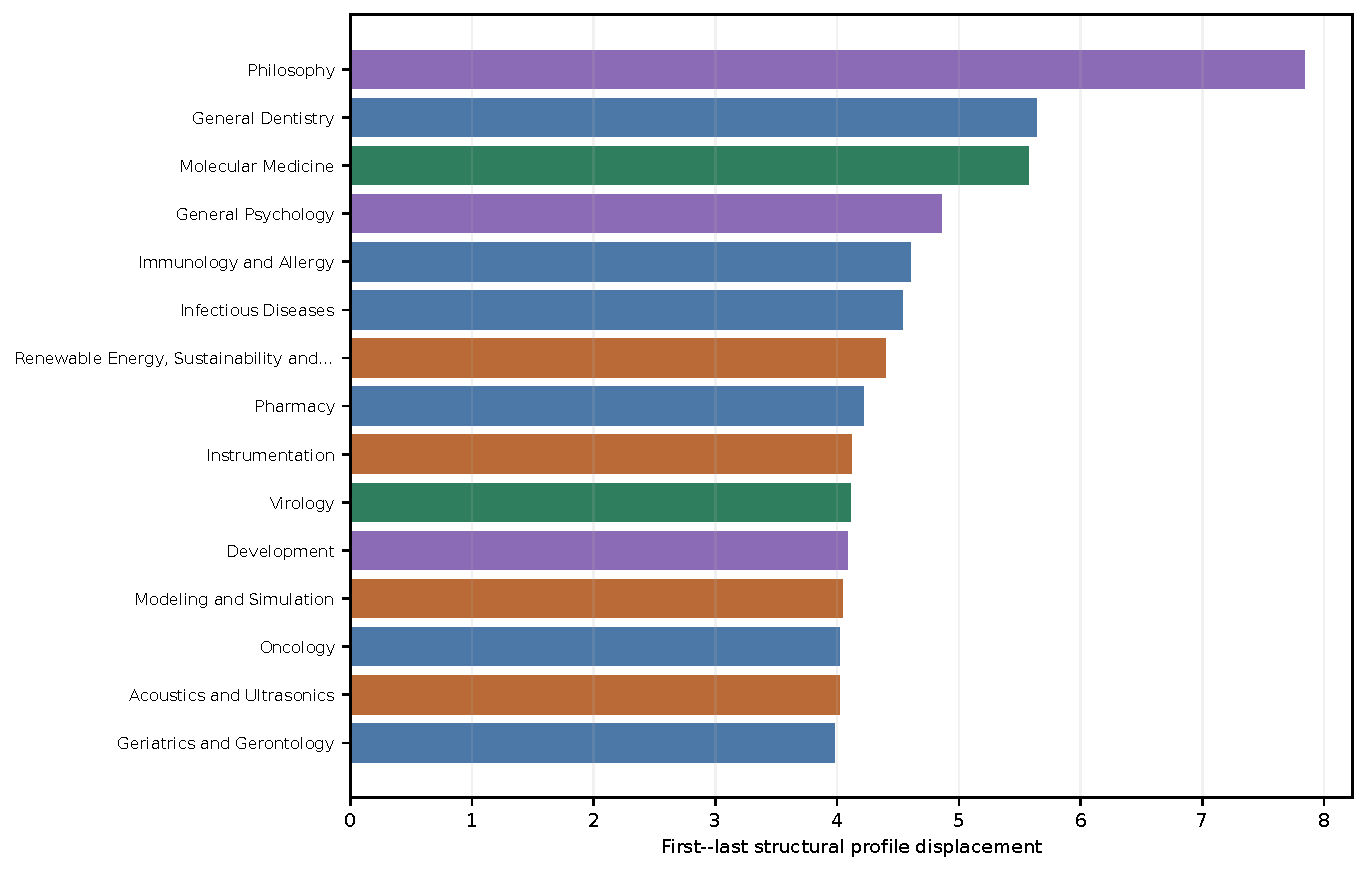
\includegraphics[width=0.93\textwidth]{figures/fig_07_most_dynamic_subfields.pdf}
\end{figure}

The drivers behind these cases are mixed. Philosophy is dominated by a sharp decrease in centroid-distance IQR, while Molecular Medicine moves in the opposite direction on the same metric. General Dentistry is driven by a decline in PCA spectral entropy. General Psychology changes mainly through reduced kNN distance variability. Immunology and Allergy and Virology change through increases in that same metric. The important point is that large temporal movement can come from different structural families.

\section{Net Semantic Displacement}

The eight-metric structural profile describes shape. A separate question is whether the semantic center of a subfield moves across the period. I measure this complementary quantity with early--late centroid drift, the cosine distance between each subfield's 2000--2004 and 2020--2024 centroids. Across analysis subfields, the median drift is 0.0045 and the maximum is 0.0384.

Centroid drift uses the same early and late windows as the first--last structural comparison, but it answers a different question. The structural metrics ask how the papers are arranged around one another. Centroid drift asks how far the average location of the subfield moves in the embedding space.

\begin{figure}[H]
\centering
\caption[Net semantic displacement extremes]{Highest and lowest early--late centroid drift by subfield. Left panel: Subfields with the highest drift (most semantically dynamic). Right panel: Subfields with the lowest drift (most stable).}
\label{fig:centroid_drift_extremes}
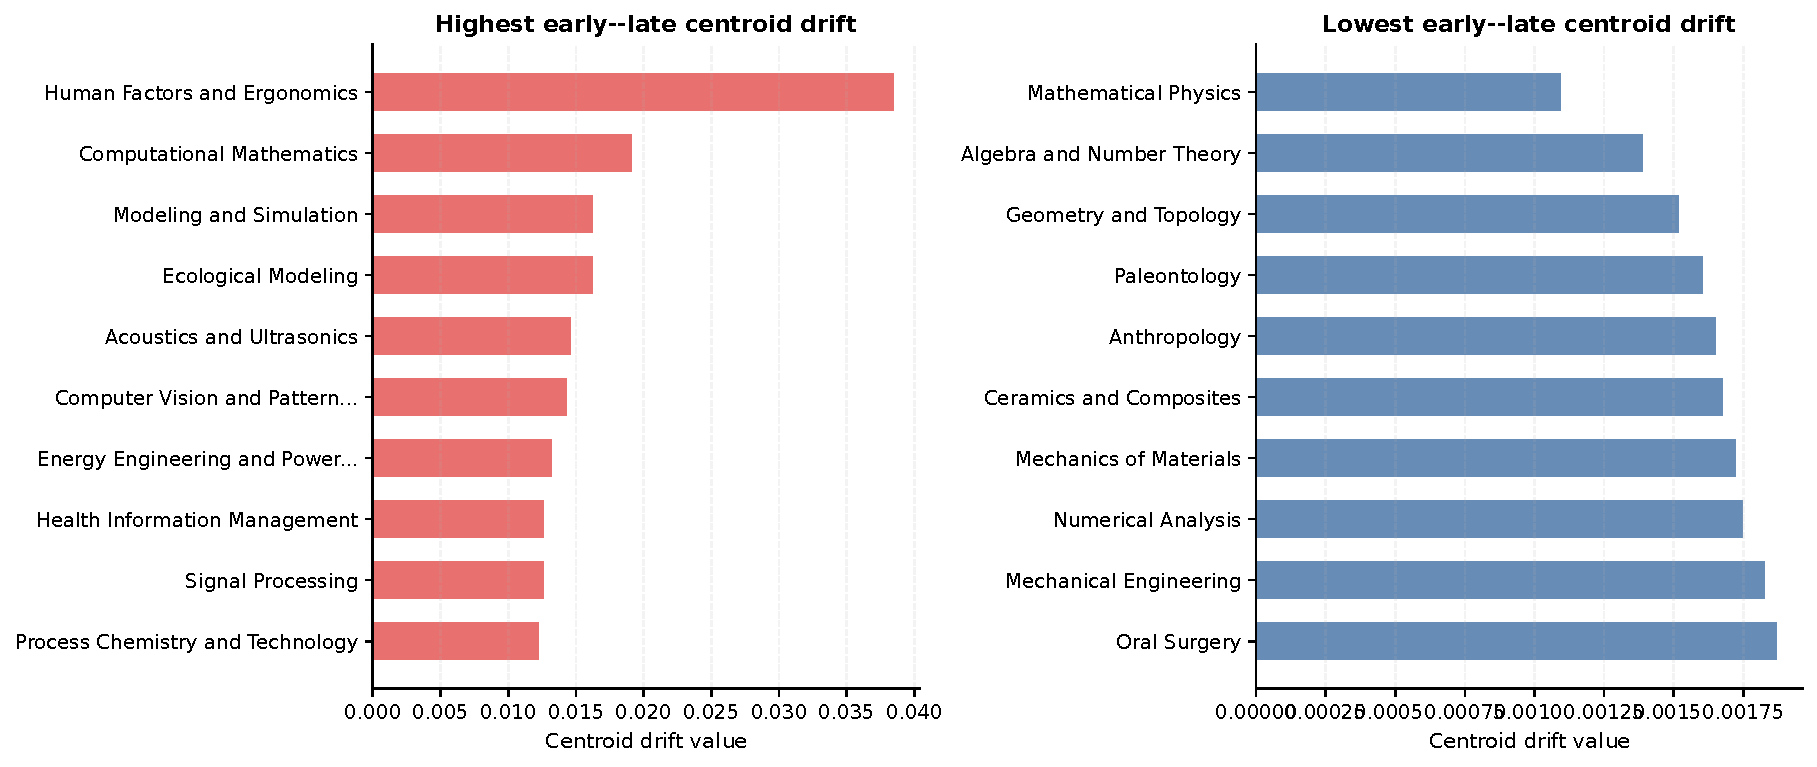
\includegraphics[width=\textwidth]{figures/fig_07_centroid_drift_extremes.pdf}
\end{figure}

The largest net displacement belongs to Human Factors and Ergonomics, followed by Computational Mathematics, Modeling and Simulation, Ecological Modeling, Acoustics and Ultrasonics, and Computer Vision and Pattern Recognition. The most stable centroids include Mathematical Physics, Algebra and Number Theory, Geometry and Topology, Paleontology, and Anthropology.

These cases are not added back into the structural profile. They answer a different diagnostic question after structural shape has already been measured. This separation matters because movement of the center and change in the internal shape are not the same result. A subfield can move in semantic location while keeping a similar profile, or it can reorganize internally while its center remains relatively stable.

\section{Static Shape Versus Temporal Trajectories}
\label{sec:static-dynamic-trajectories}

The useful part of clustering is compression. Static morphology clusters the 241 analysis subfields by eight robust-scaled full-period structural metrics. Dynamic morphology clusters the 240 complete subfields by the slopes of the same eight metrics across windows. This comparison asks whether full-period shapes or temporal trajectories form clearer descriptive groups.

In both cases, clusters are interpretive summaries rather than natural kinds or a replacement for continuous profile space. The selected static solution uses Ward hierarchical clustering, Euclidean distance, robust median/IQR scaling, and \(k=5\) \parencite{ward1963hierarchical}. Its silhouette is \(0.174\) \parencite{rousseeuw1987silhouettes}, so static morphology is better read as a continuous profile space than as a set of separated classes. The selected dynamic solution uses average-link hierarchical clustering with correlation distance at \(k=4\). It has silhouette \(=0.396\) and mean subsample ARI \(=0.725\) \parencite{hubert1985comparing}, making it a clearer and more stable descriptive compression.

\begin{figure}[H]
\centering
\caption[Dynamic temporal typology profile heatmap]{Dynamic temporal-trajectory typology profiles. Values are mean standardized linear slopes of the eight windowed structural metrics.}
\label{fig:dynamic_typology_profile_heatmap}
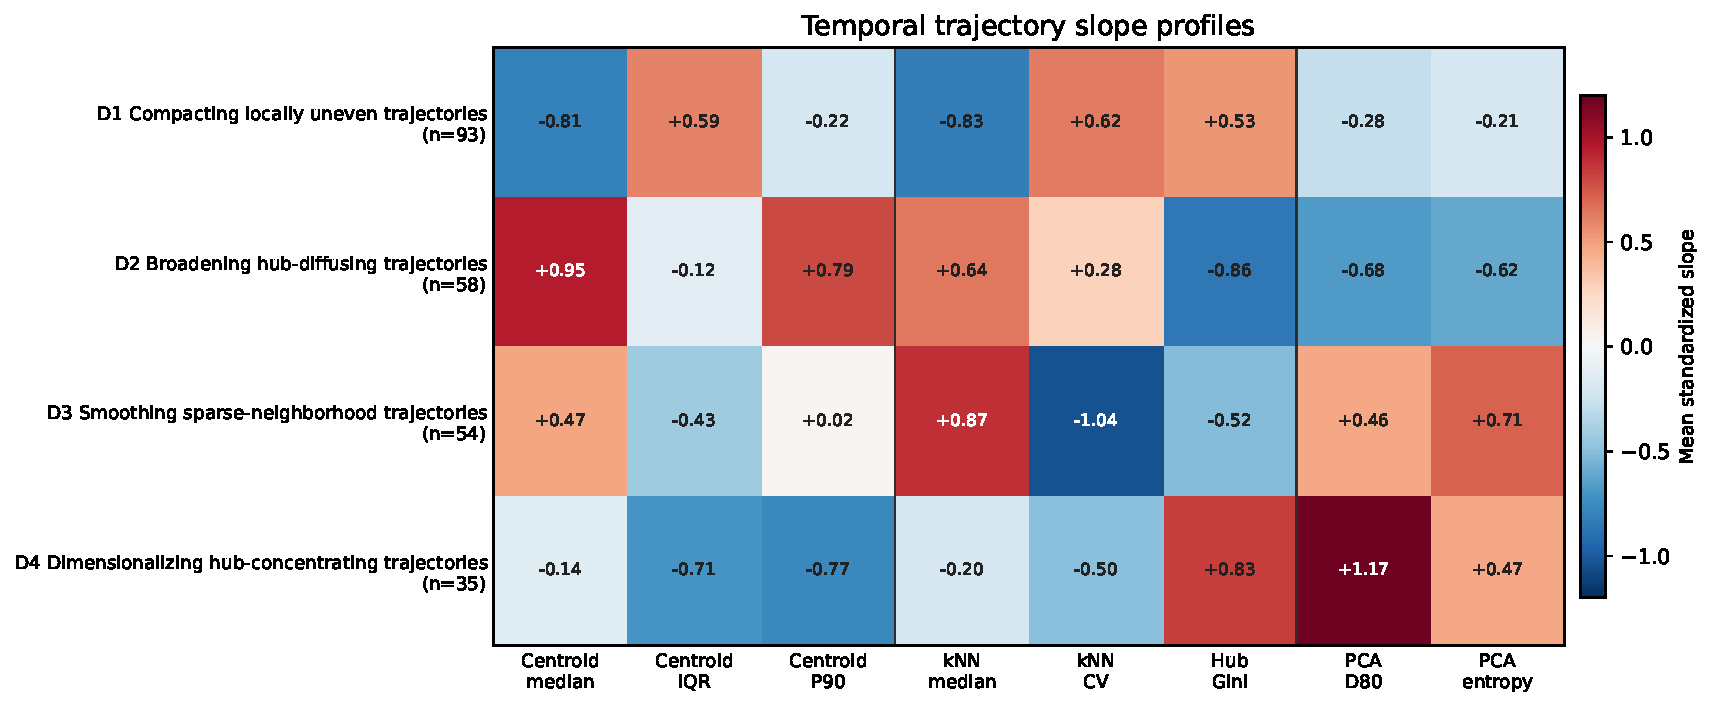
\includegraphics[width=\textwidth]{figures/fig_09_dynamic_typology_profile_heatmap.pdf}
\end{figure}

The four dynamic groups describe movement patterns. D1, with 93 subfields, contracts in centroid and kNN distance while local unevenness and hub concentration rise. D2, with 58 subfields, broadens while hubness and spectral complexity decline. D3, with 54 subfields, becomes sparser in local distance while local unevenness and hubness fall. D4, with 35 subfields, increases PCA dimensionality and hubness while outer spread and local variability fall. These labels are shorthand for slope profiles, not a new taxonomy.

The dynamic typology is useful because it gives names to repeated trajectory patterns. It should not be read as a new classification of science. The groups depend on the selected corpus, representation, metrics, windows, scaling, and clustering procedure. Their value is descriptive compression, not causal explanation. The main temporal result is that structural profiles move in heterogeneous but measurable ways, while centroid drift supplies a separate view of semantic displacement.


\chapter{Morphological Similarity, Convergence and Divergence}
% Chapter 8: Morphological Similarity, Convergence and Divergence

\section{Turning Profiles into Relations}

Two disciplines are morphologically similar when their embedding-space metric profiles are close after robust standardization. This is not document-level semantic similarity: two fields can be morphologically close without studying the same topics, using the same vocabulary, citing the same work, or belonging to the same institutional tradition. Their paper distributions have similar structural shape under the reduced metric representation.

Static similarity uses the full eleven-metric core from Chapter~5. For each metric, values are centered by the cross-subfield median and scaled by the interquartile range; field and domain profiles are averages of the robust-scaled subfield profiles. The primary distance used below is Euclidean distance between these standardized profiles, because it preserves magnitude differences in dispersion, local density, hubness, spectral structure, and full-period temporal indicators.

Temporal convergence and divergence use the eight structural metrics recomputed inside each five-year window. The three full-period temporal indicators are excluded from windowed pairwise distances because they are already summaries over time. Operationally, convergence means that the distance between two windowed profiles decreases from 2000--2004 to 2020--2024; divergence means that it increases.

\section{Static Similarity Across Disciplines}

The static field-level distance matrix gives a compact view of profile-space structure. If OpenAlex domains fully aligned with morphology, the diagonal domain blocks would be uniformly light and the off-block regions uniformly dark. Figure~\ref{fig:field_static_distance_heatmap} shows a weaker pattern. Some domain blocks are internally coherent, but many nearest profile-space relations cross domain boundaries.

\begin{figure}[H]
\centering
\caption[Pairwise field morphological distances]{Pairwise morphological distance between fields. Distances are computed from robust-scaled eleven-metric profiles; lower values indicate more similar morphology.}
\label{fig:field_static_distance_heatmap}
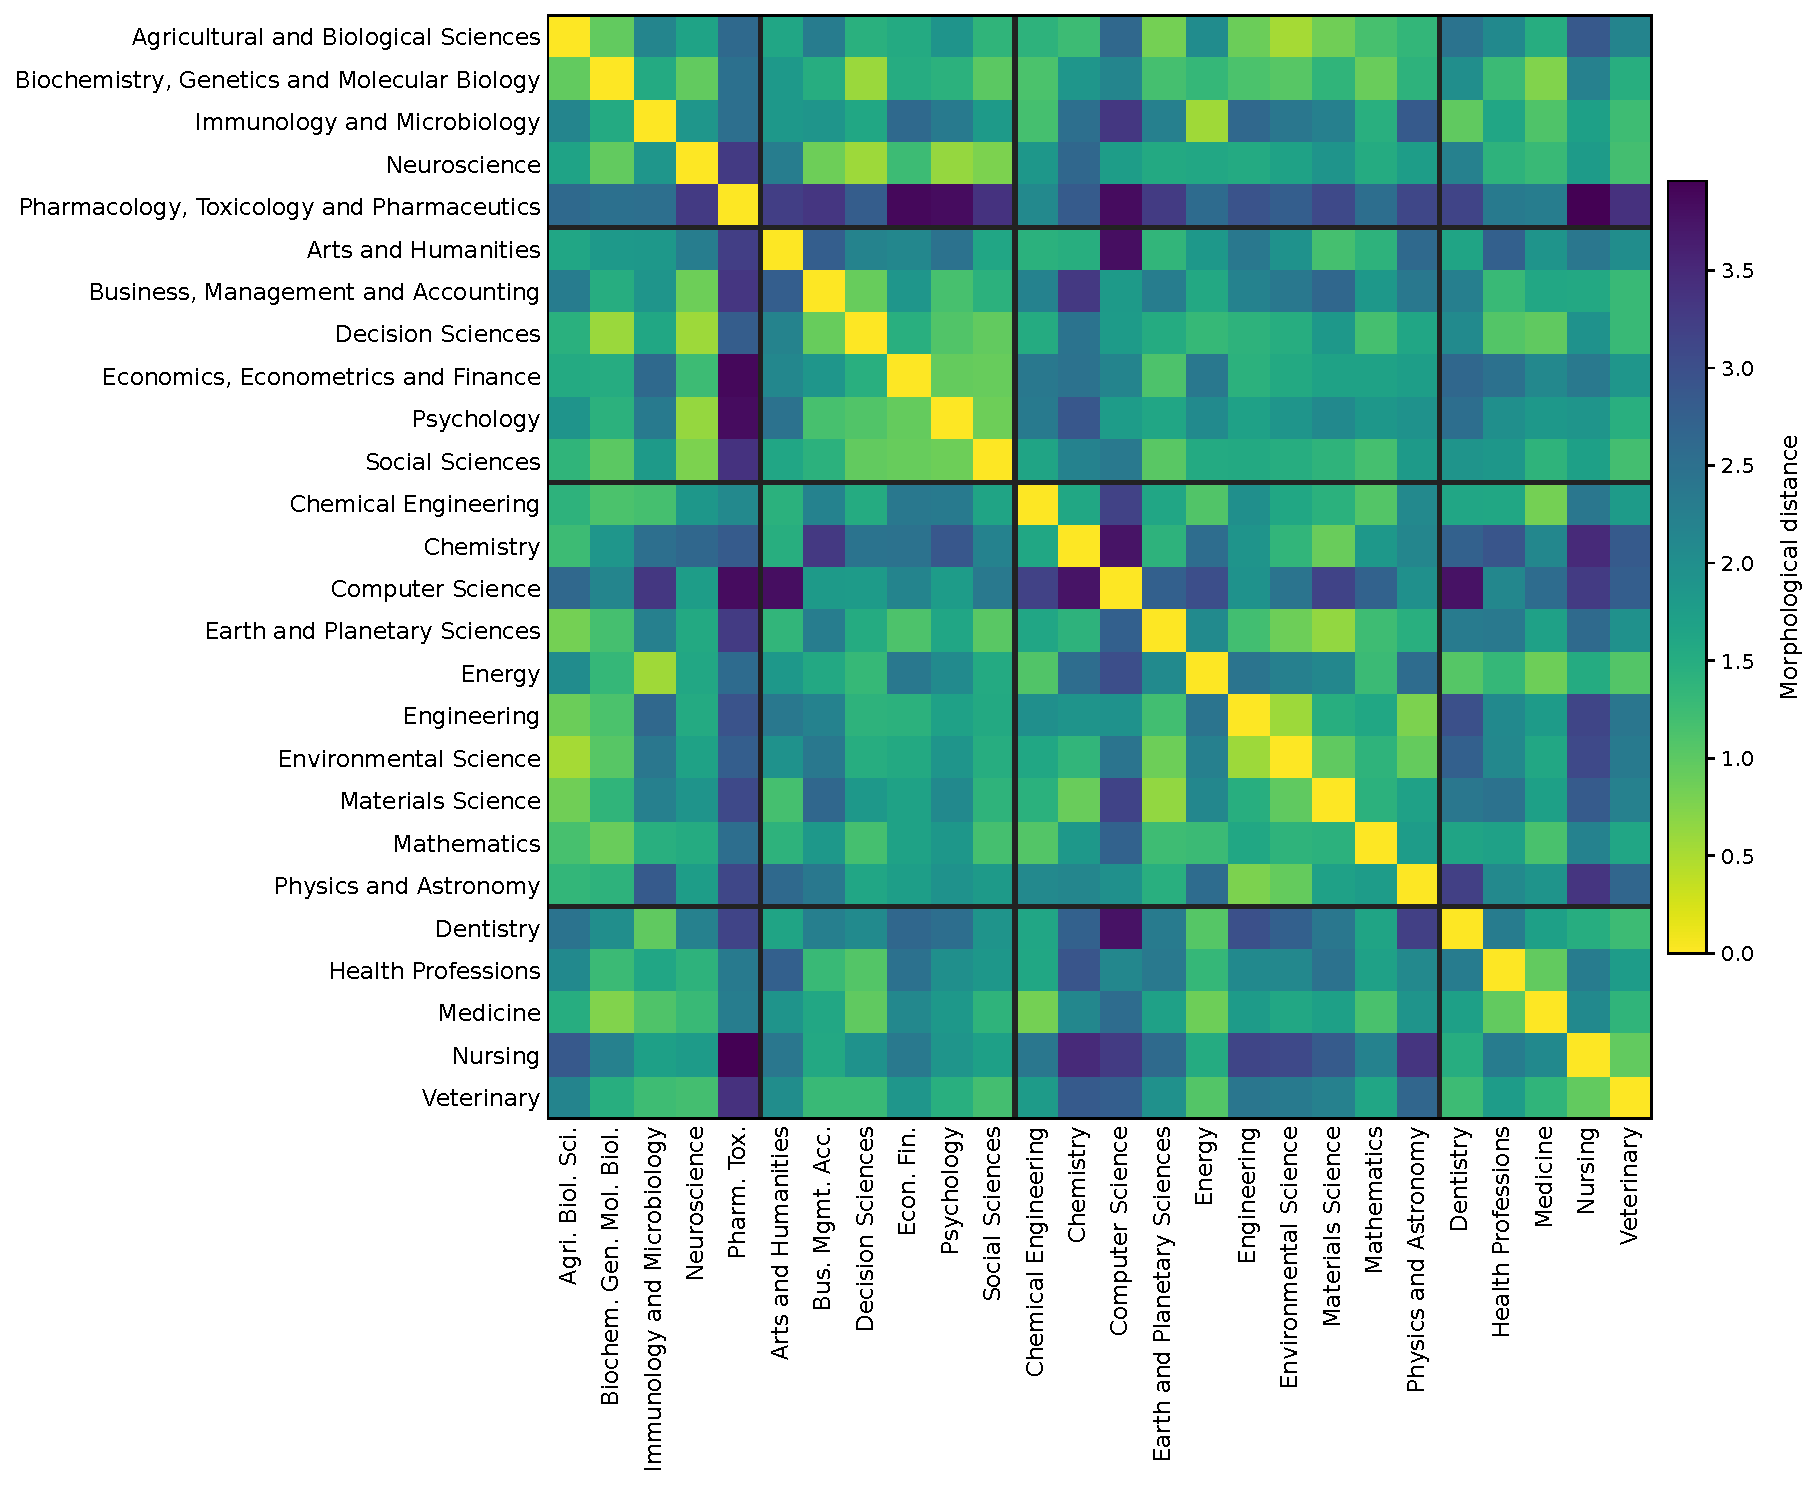
\includegraphics[width=\textwidth]{figures/fig_08_field_static_distance_heatmap.pdf}
\end{figure}

The closest Euclidean field pairs are not simply within-domain neighbors. Biochemistry, Genetics and Molecular Biology is closest to Medicine; Neuroscience is closest to Psychology; Chemical Engineering is close to Medicine; and Agricultural and Biological Sciences is close to Materials Science. These links do not imply shared content. They mean that the fields have similar standardized levels of compactness, dispersion, hubness, spectral structure, and temporal indicators. The comparison makes shape relations visible without turning them into topic relations.

Figure~\ref{fig:domain_pair_distance_structure} replaces the binary within--cross contrast with a domain-pair view. Within-domain field pairs have a lower overall median distance than cross-domain pairs, \(1.90\) versus \(2.20\), but the domain cells show where that average comes from. Social Sciences are the most internally coherent domain, while the closest cross-domain relation is between Life Sciences and Health Sciences. At field level, 18 of 26 fields have their nearest morphological neighbor outside their own domain. This is the chapter's clearest evidence that formal domains and morphology do not give the same structure.

\begin{figure}[H]
\centering
\caption[Domain-pair morphological distance structure]{Domain-pair morphological distance structure. Panel A reports median field-pair distances for each pair of OpenAlex domains; Panel B counts fields whose nearest morphological neighbor lies inside or outside their own domain.}
\label{fig:domain_pair_distance_structure}
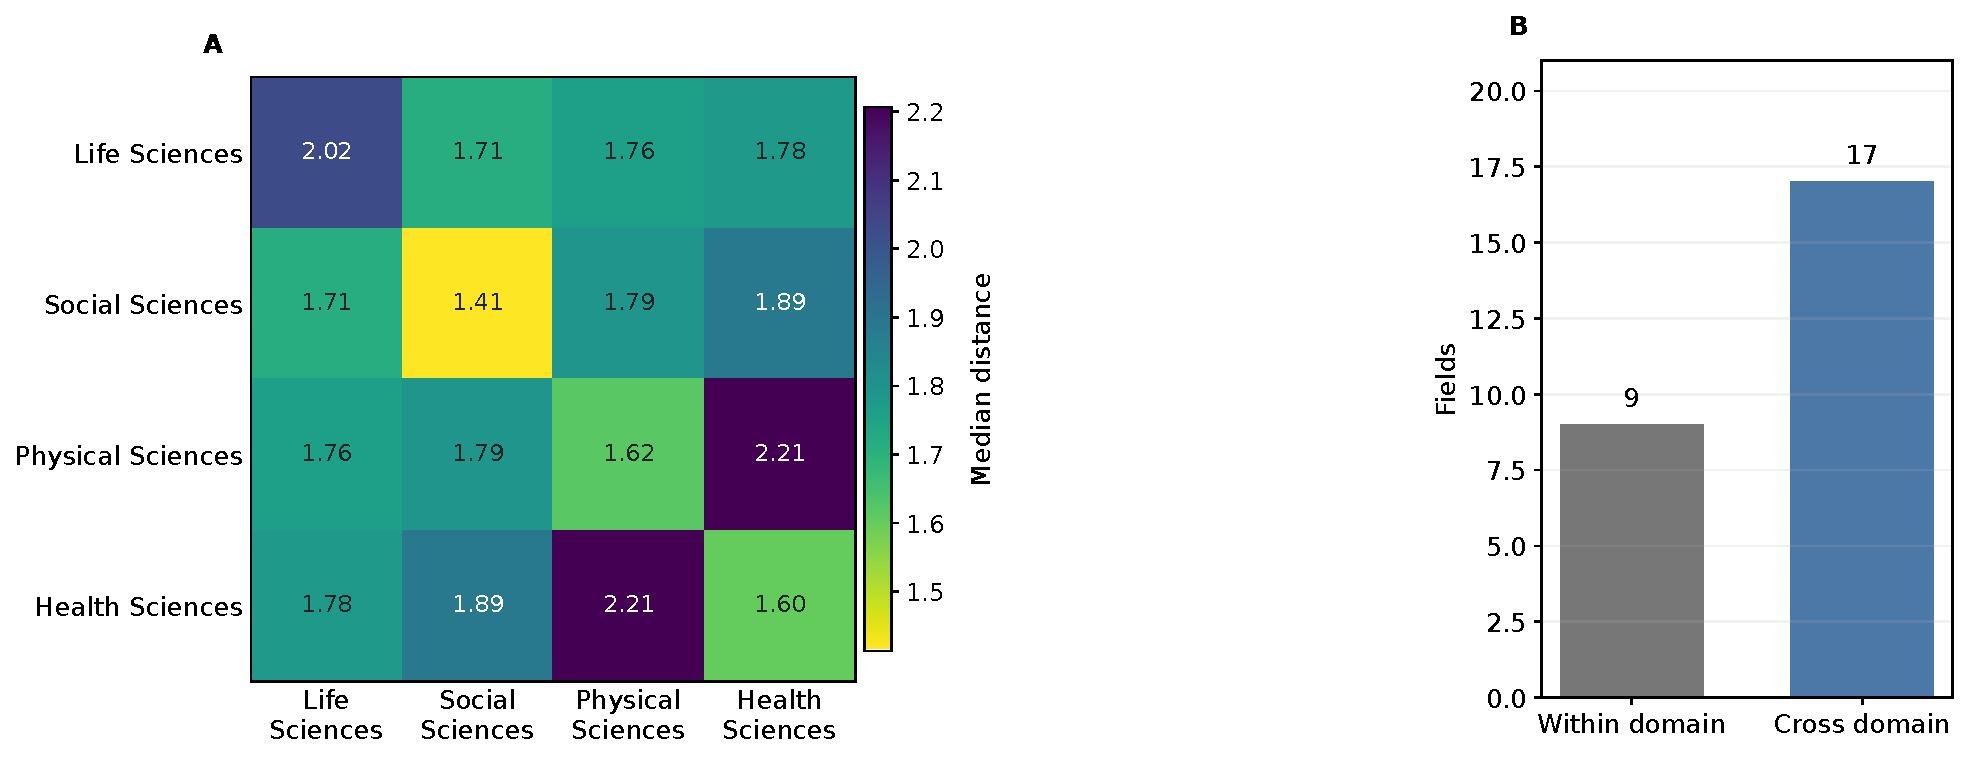
\includegraphics[width=\textwidth]{figures/fig_08_domain_pair_distance_structure.pdf}
\end{figure}

Figure~\ref{fig:field_nearest_neighbor_ring} makes the same result more concrete by turning the distance matrix into a directed nearest-neighbor map. Each arrow starts in a field and points to the field with the closest full-period morphology profile; dark arrows cross OpenAlex domain boundaries and grey arrows remain inside the same domain. The circular layout preserves domain membership, so the figure should be read as a stress test of the taxonomy: if domain labels fully organized morphology, most arrows would stay within their own sector.

\begin{figure}[H]
\centering
\caption[Directed field nearest-neighbor map]{Directed nearest-neighbor map between fields in morphology-profile space. Arrows point from each field to its nearest morphological neighbor under the robust-scaled eleven-metric distance; dark arrows indicate cross-domain nearest neighbors and grey arrows indicate within-domain nearest neighbors. Node size is proportional to the number of included subfields.}
\label{fig:field_nearest_neighbor_ring}
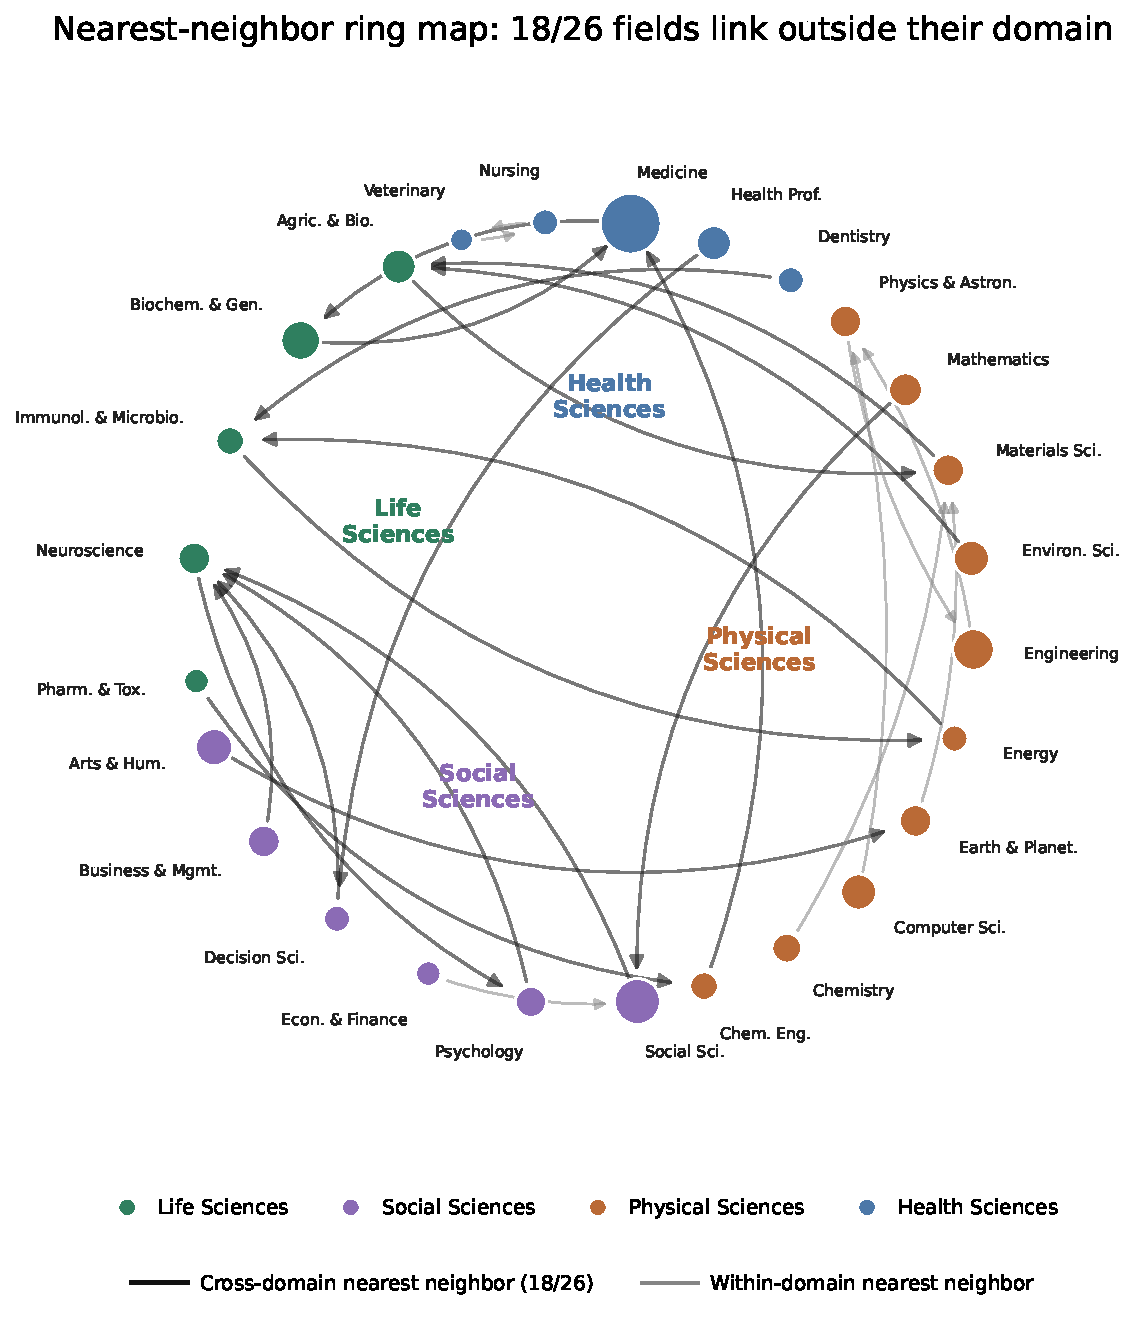
\includegraphics[width=\textwidth]{figures/fig_08_field_neighbor_variant_02_domain_ring.pdf}
\end{figure}

The map clarifies three aspects that are harder to see in the heatmap. First, cross-domain similarity is not a marginal exception but the dominant local relation: the dark chords are spread around the ring rather than concentrated in a single anomalous block. Second, several relations are reciprocal, including Medicine with Biochemistry, Genetics and Molecular Biology, Neuroscience with Psychology, Energy with Immunology and Microbiology, and Nursing with Veterinary. These reciprocal links identify local morphological pairs, not merely one-sided approximations. Third, some fields act as attractors for multiple neighbors. Materials Science receives links from Agricultural and Biological Sciences, Chemistry, and Earth and Planetary Sciences, while Neuroscience receives links from Business, Management and Accounting, Decision Sciences, and Social Sciences. The interpretation is therefore not that domains are irrelevant, but that domain membership is an incomplete predictor of field shape: morphology produces local affinities, bridges, and asymmetric pulls that the domain-level taxonomy smooths over.

\section{Convergence and Divergence Over Time}

The temporal picture is not global convergence. Across all 325 field pairs, mean Euclidean distance rises from \(1.44\) in 2000--2004 to \(1.81\) in 2020--2024. The same upward movement appears within domains, from \(1.39\) to \(1.70\), and across domains, from \(1.46\) to \(1.85\). Field-level morphology space becomes more separated on average, even though many individual pairs move closer. This supports the main argument because it separates average differentiation from selective convergence.

\begin{figure}[H]
\centering
\caption[Temporal field-pair distance trajectories]{Mean field-pair morphological distance across five-year windows using the eight windowed structural metrics.}
\label{fig:temporal_distance_trajectories}
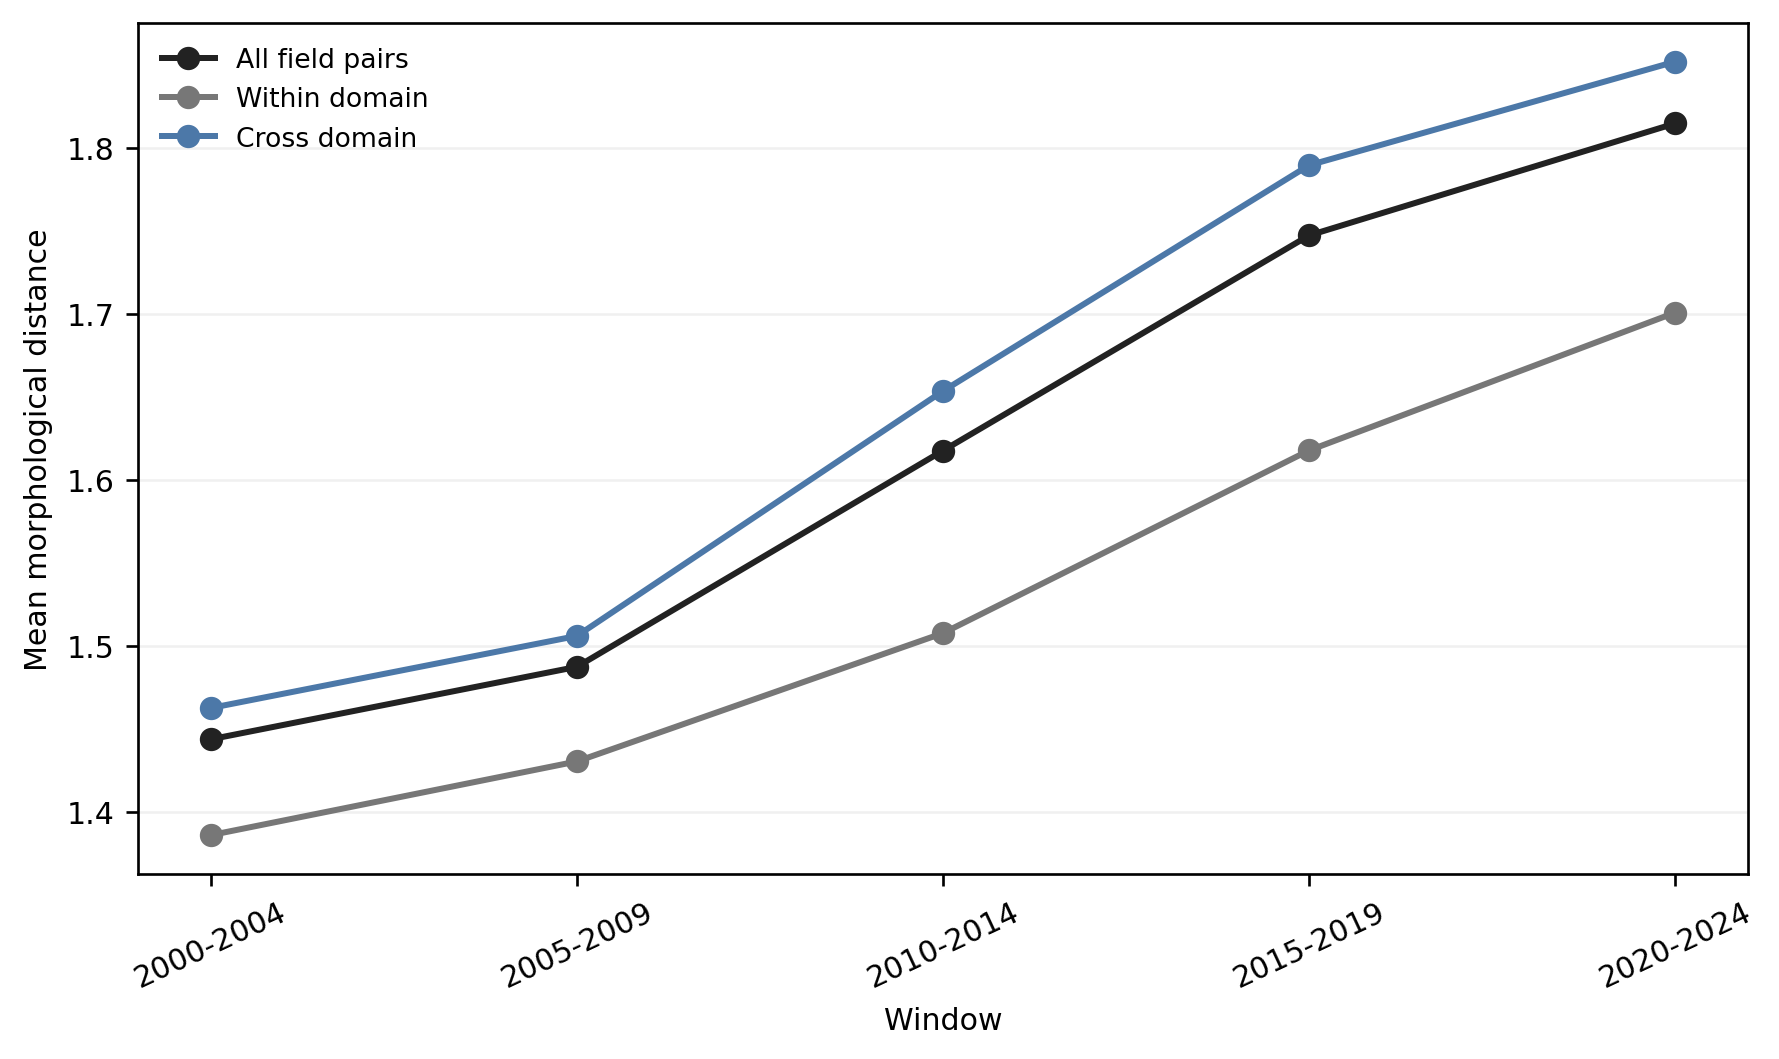
\includegraphics[width=0.88\textwidth]{figures/fig_08_temporal_distance_trajectories.png}
\end{figure}

This average expansion coexists with selective convergence: 97 field pairs decrease in distance, while 228 increase. The strongest convergences tend to involve shared declines in local distance and spectral dimensionality. Materials Science and Mathematics move from \(1.75\) to \(0.85\); Decision Sciences and Environmental Science from \(1.67\) to \(0.82\); and Economics, Econometrics and Finance and Psychology from \(1.53\) to \(0.70\). These are relative movements in metric-profile space, not evidence of intellectual merger.

\begin{figure}[H]
\centering
\caption[Strongest field convergence and divergence]{Strongest field-level convergence and divergence under Euclidean profile distance. Open markers are initial distances and filled markers are final distances; labels show final-minus-initial change.}
\label{fig:field_convergence_divergence_pairs}
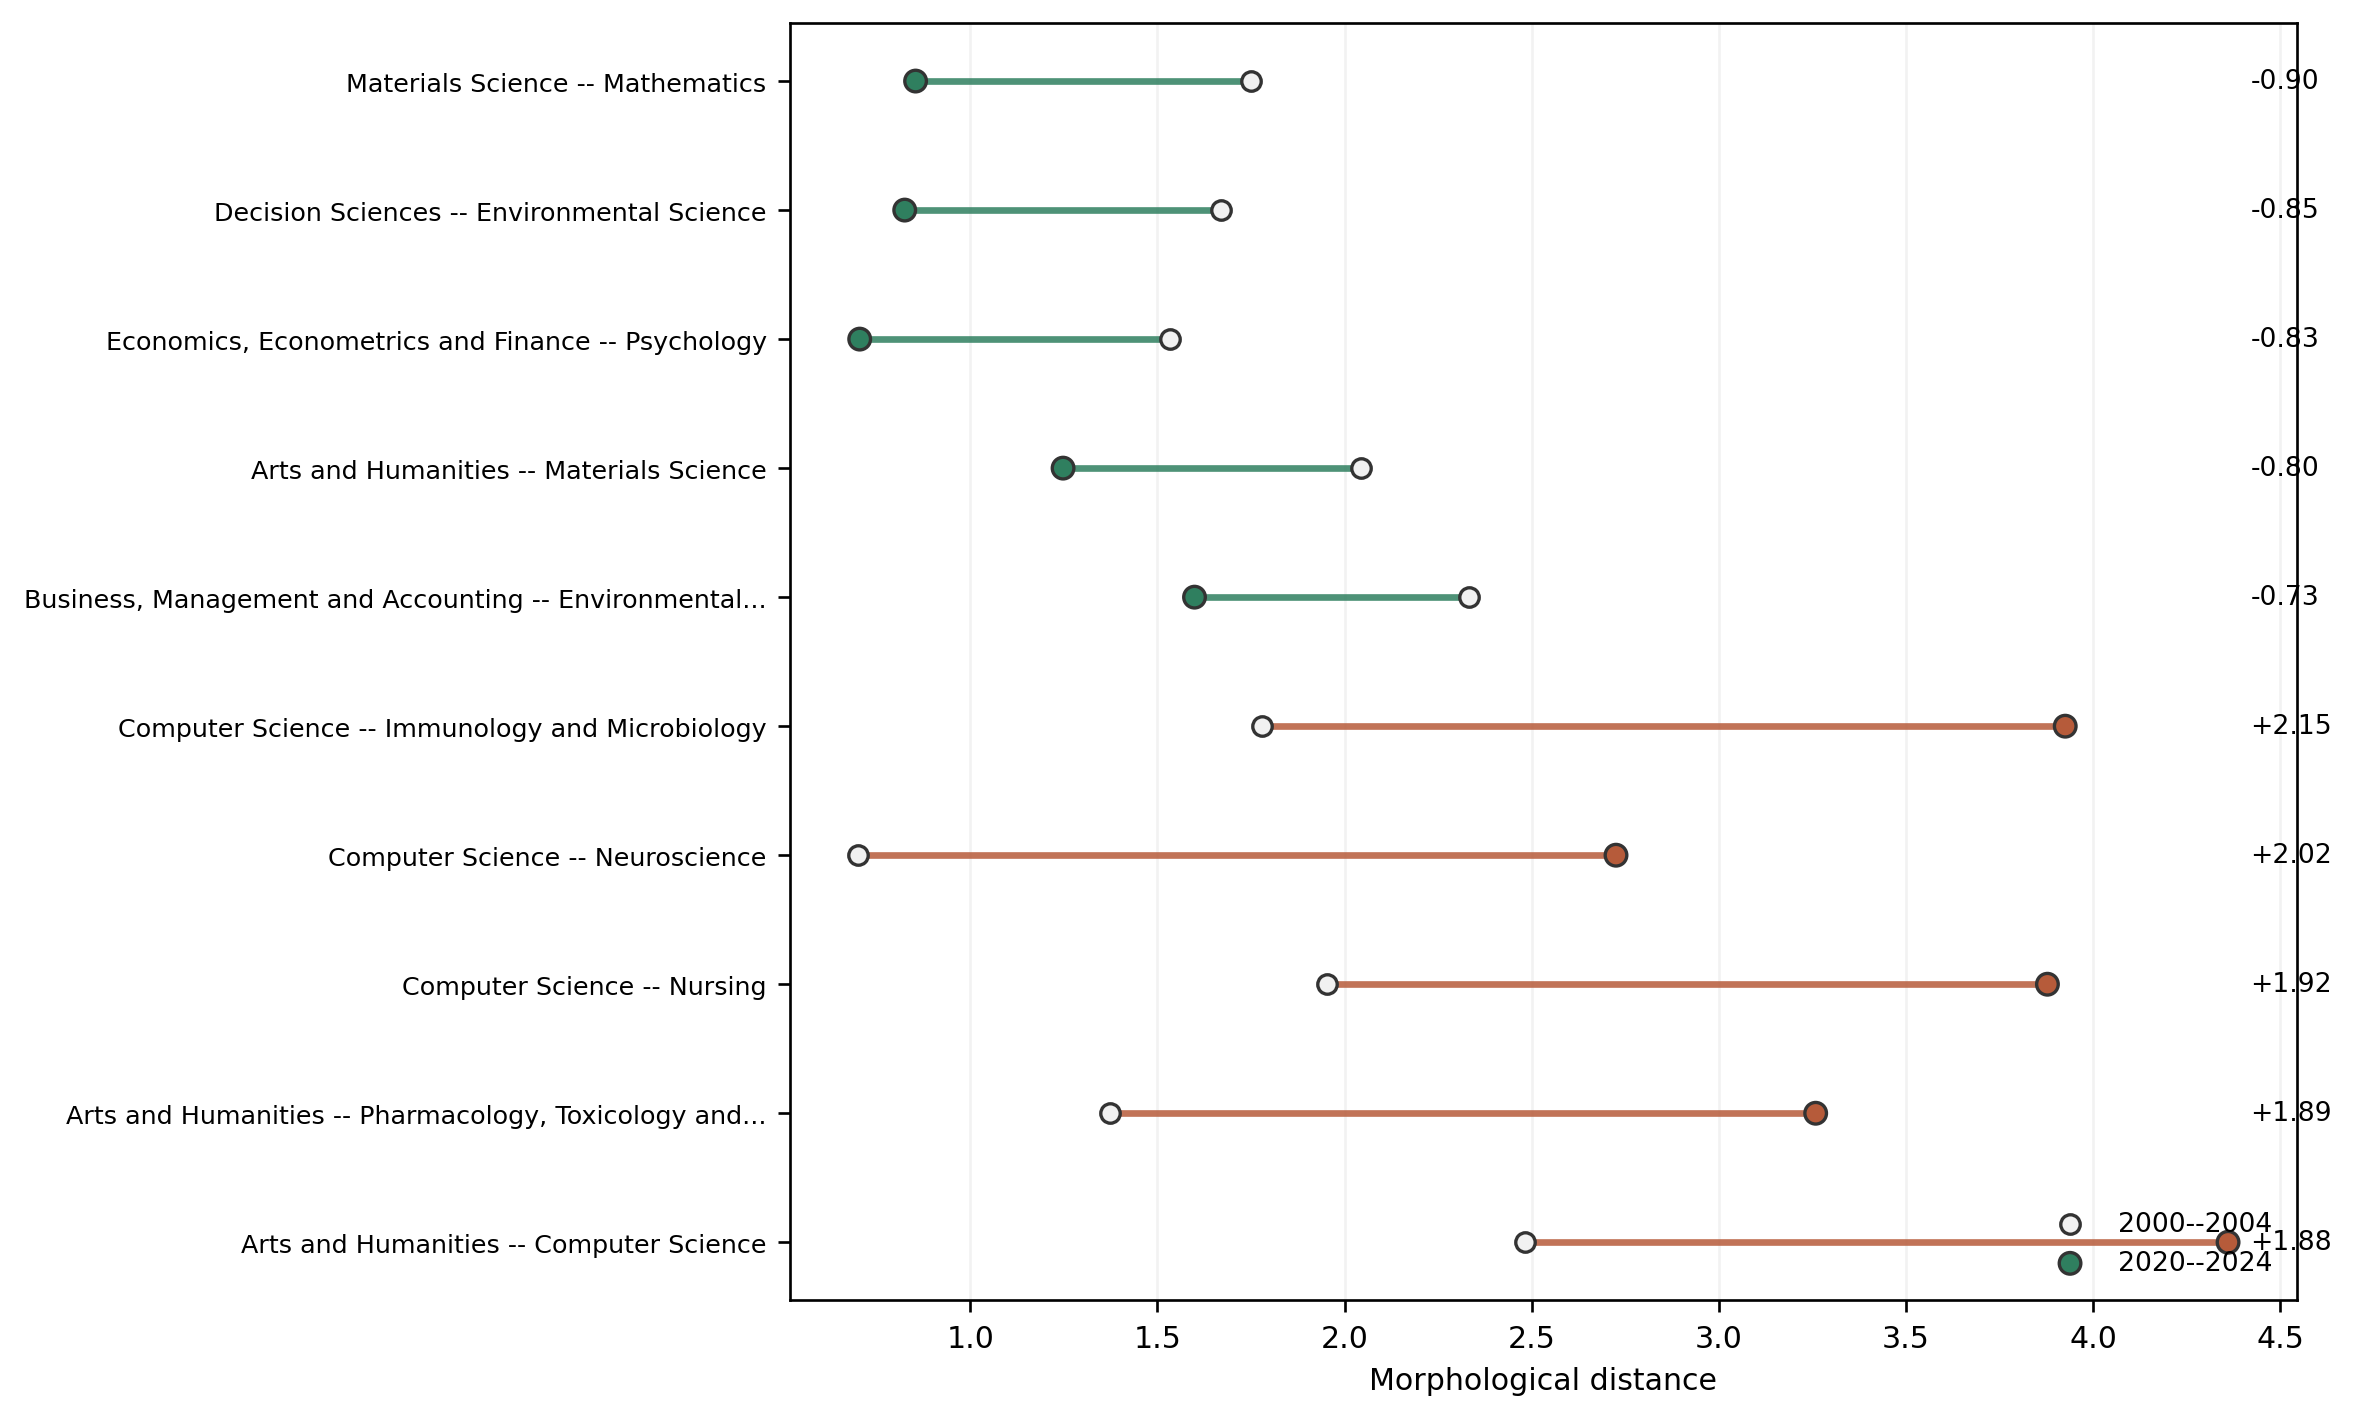
\includegraphics[width=\textwidth]{figures/fig_08_field_convergence_divergence_pairs.png}
\end{figure}

\begin{table}[H]
\centering
\caption[Field convergence and divergence drivers]{Selected field-level convergence and divergence cases}
\label{tab:field_convergence_drivers}
\scriptsize
\begingroup
\setlength{\tabcolsep}{2.5pt}
\begin{tabular}{@{}>{\raggedright\arraybackslash}p{0.27\textwidth} >{\raggedright\arraybackslash}p{0.14\textwidth} >{\raggedleft\arraybackslash}p{0.10\textwidth} >{\raggedright\arraybackslash}p{0.39\textwidth}@{}}
\hline
\textbf{Pair} & \textbf{Relation} & \textbf{$\Delta$ dist.} & \textbf{Largest profile movements} \\
\hline
Materials Sci. -- Mathematics & Converges & -0.90 & Materials Sci.: kNN median -1.5, PCA entropy -1.2; Mathematics: centroid IQR -0.74, PCA entropy -0.73 \\
Decision Sci. -- Environmental Sci. & Converges & -0.85 & Decision Sci.: PCA entropy -1.1, PCA D80 -1.1; Environmental Sci.: kNN median -1.5, PCA D80 -1.2 \\
Economics \& Finance -- Psychology & Converges & -0.83 & Economics \& Finance: PCA D80 -1.2, kNN median -1.1; Psychology: PCA D80 -1.2, PCA entropy -0.99 \\
Computer Sci. -- Immunol. \& Microbio. & Diverges & +2.15 & Computer Sci.: PCA D80 -1.8, PCA entropy -1.5; Immunol. \& Microbio.: kNN median -1.5, kNN CV +1.3 \\
Computer Sci. -- Neuroscience & Diverges & +2.02 & Computer Sci.: PCA D80 -1.8, PCA entropy -1.5; Neuroscience: kNN median -0.97, PCA entropy -0.9 \\
Computer Sci. -- Nursing & Diverges & +1.92 & Computer Sci.: PCA D80 -1.8, PCA entropy -1.5; Nursing: kNN median -1.4, PCA entropy -0.99 \\
\hline
\end{tabular}
\endgroup
\par\vspace{0.15cm}
\footnotesize\textit{Note.} Distances are Euclidean distances between robust-scaled field profiles in the eight windowed structural metrics. Negative final-minus-initial distance indicates convergence; positive values indicate divergence.
\end{table}


The diverging side has a clearer protagonist. Computer Science appears in nine of the ten largest field-level Euclidean divergences, including divergences from Immunology and Microbiology, Neuroscience, Nursing, Dentistry, Energy, and Arts and Humanities. This does not mean that Computer Science becomes semantically remote in topic space; its windowed morphology changes in a way that separates its standardized structural profile from many other fields.

\section{Nearest Neighbors, Bridges, and Isolates}

Nearest-neighbor relations make the matrix interpretable without turning this chapter into a typology. Some neighbors are expected: Chemistry and Materials Science are close, and Nursing and Veterinary are each other's nearest field-level neighbors among the more isolated Health Sciences fields. Other neighbors cross domains: Medicine is nearest to Biochemistry, Genetics and Molecular Biology; Psychology is nearest to Neuroscience; and Energy is nearest to Immunology and Microbiology.

These are bridges only in a morphological sense. They indicate similar profile shape, not collaboration or topical overlap. The strongest static isolates are equally important. Computer Science has the largest nearest-neighbor distance among fields: even its closest field-level neighbor, Physics and Astronomy, remains at distance \(2.75\). It also appears in the farthest static pairs, especially against Pharmacology, Toxicology and Pharmaceutics, Dentistry, Chemistry, Arts and Humanities, and Veterinary.

At subfield level, the same relational logic becomes more extreme. Ecology and Materials Chemistry are the closest static subfield pair, followed by Nutrition and Dietetics with Pulmonary and Respiratory Medicine. The strongest temporal subfield convergence is concentrated around Philosophy, which appears in all ten top Euclidean convergence pairs; the strongest divergence is concentrated around Molecular Medicine, which appears in all ten top Euclidean divergence pairs. These cases show that the most dramatic relational movements occur below the broad field level.

Morphological similarity is a structural comparison under a specific representation. A low distance means that two aggregate metric profiles are close after robust scaling; a high distance means that their profiles differ on one or more metric dimensions. The value of the chapter is relational and descriptive: it shows which scientific regions resemble, approach, or separate from one another in morphological profile space, providing groundwork for Chapter~9.

\paragraph{What this result means.}
Morphological similarity only partly follows taxonomy. Many fields are closest in shape to fields outside their own domain. This does not mean those fields study the same topics; it means their embedded paper distributions are arranged in similar ways. Shape and taxonomic membership are related, but not the same.


\chapter{Exploratory Morphological Typologies}
% Chapter 9: Exploratory Morphological Typologies
% Focus: Clustering scientific disciplines into descriptive typologies based on the 11 core embedding-space metrics.
% Document Feeds: docs/TFM_summary.md, docs/reduced_metric_core.md
% Outputs: outputs/04_reduced_metric_core/ (for the 11 metrics), potential clustering tables/plots.
% Citations: Reminders to cite unsupervised clustering methods (e.g. Hierarchical Clustering, K-Means) and typological philosophy.
% IMPORTANT constraints:
%   - Clustering is strictly exploratory and must be based ONLY on the reduced 11 embedding-space metrics, NOT UMAP coordinates.
%   - The clusters must be interpreted as descriptive typologies (conceptual guides), NOT as natural or objective categories of science.
%   - There is NO standalone visualization chapter; UMAP projections and visual density maps are integrated inside the relevant chapters as interpretive support.
% TODO: Run exploratory clustering on the 11-metric profiles and export the resulting cluster members and dendrograms.

\noindent This chapter presents an exploratory clustering analysis of scientific disciplines. Using the eleven core high-dimensional morphological metrics, we group subfields with structurally similar profiles to build descriptive typologies. This unsupervised typology provides a heuristic framework to understand the shared morphological features of modern scientific research.

% TODO: Outline the clustering methodology (e.g., Hierarchical Agglomerative Clustering or K-Means on the 11-metric profiles).
% TODO: Justify clustering directly in the original 768-D derived metric space (excluding UMAP coordinates to prevent distortion).
% TODO: Present the descriptive typologies, analyzing the key morphological traits that define each cluster.
% TODO: Emphasize the epistemological status of clusters as descriptive typologies rather than absolute, objective boundaries.
% TODO: Integrate interpretive UMAP visualizations and density plots directly here to illustrate cluster coherence in 2D.


\chapter{Discussion}
% Chapter 10: Discussion

\section{What It Means to Measure the Shape of Science}

The thesis shifts the object of measurement from the content of a field to the geometry of its embedded paper distribution. A field is not treated as a list of topics, a citation community, a productivity unit, or a point in a predefined taxonomy. It is treated as a distribution of title--abstract records in a shared SPECTER2 embedding space. Its morphology is the way that distribution occupies the space: how dispersed it is, how tightly its local neighborhoods are packed, how concentrated those neighborhoods are around hubs, how many spectral directions summarize its variation, and how its position changes over time.

This move makes the analysis complementary to standard science maps. Topic models ask what texts are about. Citation networks ask how works, authors, venues, or fields are connected. Bibliometric indicators often ask how much is produced, cited, or recognized. Embedding-space morphology asks a narrower geometric question: given a representation of scientific documents, what structural shape does a field's collection of papers have?

That question is conditional by design. The measurements are properties of a balanced OpenAlex title--abstract corpus, grouped by OpenAlex primary-topic subfields, embedded with SPECTER2, and measured in the original 768-dimensional representation space. This conditionality is not a weakness to hide; it is what makes the result reproducible. The thesis does not claim to reveal the true map of science. It measures one aspect of scientific organization while keeping the data source, taxonomy, representation model, sampling design, and geometric assumptions visible.

\section{Static Shape, Temporal Change, and Semantic Location}

Chapter~6 establishes the first empirical layer: broad domains have morphological tendencies, but they do not determine morphology. Physical Sciences are generally more dispersed and spectrally extended. Health Sciences are more locally dense and hub-concentrated. Social Sciences and Life Sciences occupy less extreme average positions on several metrics. Yet those averages are blunt summaries. Field-level and subfield-level profiles vary substantially within each domain, and the most atypical subfields are extreme for different reasons: dispersion, novelty, local density, hubness, spectral structure, or combinations of them.

Chapter~7 adds time. Across the population of subfields, median centroid distance, median kNN distance, and PCA \(D_{80}\) decline from the first to the last window, while local distance variability can rise and hubness does not move uniformly. Temporal evolution is therefore not a simple story of fields becoming smaller, denser, or more homogeneous. A subfield may become locally compact while becoming more uneven; another may reduce spectral dimensionality while losing hub concentration; another may move far in centroid space without sharing the same structural trajectory.

Chapter~8 turns morphology into a relation. Field-level profile distances show that taxonomy captures part of the structure, but many nearest morphological neighbors cross domain boundaries. The average field-pair distance increases from 2000--2004 to 2020--2024, so profile space becomes more separated rather than globally convergent. That average divergence coexists with selective convergence: some field pairs move closer through shared changes in local distance and spectral dimensionality, while many others move apart.

Chapter~9 compresses these findings into typologies. Static morphology is weakly clustered. The selected Ward \(k=5\) typology has silhouette \(=0.133\), which supports descriptive anchors rather than natural categories. Temporal trajectories separate more clearly, with silhouette \(=0.396\) and mean subsample ARI \(=0.725\). Subfields are easier to group by how their morphology changes than by their full-period shape.

The centroid and hybrid sensitivity checks complete the interpretation. Clustering subfield centroid embeddings separates somewhat more clearly and aligns more strongly with OpenAlex domains than morphology clustering does. Hybrid clustering becomes highly stable when semantic location receives substantial weight. These results do not undermine the morphology typology; they show why semantic location and morphology must remain separate. A field's position in embedding space is not the same as the shape of its distribution around that position.

\section{Methodological Contributions}

The first contribution is a reproducible corpus design for embedding-based science mapping. The thesis builds a synchronized OpenAlex title--abstract corpus covering 2000--2024, with annual balancing across subfield-year cells. This strategy reduces the dominance of high-volume subfields and makes temporal and cross-sectional comparisons more defensible, while making the limits of the empirical object explicit.

The second contribution is the disciplined use of SPECTER2 as an analytical geometry. Quantitative metrics are computed in the original embedding space rather than on UMAP, PCA, or other low-dimensional projections. This prevents visual maps from silently becoming measurement spaces and keeps representation, measurement, and communication apart.

The third contribution is the reduced eleven-metric morphology core. The metric set covers global dispersion, local density and hubness, spectral structure, and temporal movement. No single metric is asked to summarize a field. Morphology is treated as a profile, which makes it possible to see why a field can be dispersed but locally regular, compact but hub-concentrated, or spectrally simple while temporally novel.

The fourth contribution is the separation of static morphology, temporal morphology, morphological similarity, and semantic-location clustering. A single two-dimensional display can make position, distance, cluster, and category appear to be the same object. The thesis keeps them apart: static profiles describe full-period shape, temporal trajectories describe windowed change, similarity compares profiles between units, and centroid clustering checks semantic location rather than shape.

The fifth contribution is interpretive conservatism in clustering. Static clusters are treated as typological anchors because they are weak. Temporal clusters are treated as dynamic tendencies because they are clearer but still exploratory. Centroid and hybrid clusters are used as sensitivity evidence, not as replacements for morphology. The point is not merely technical; it is a way to use clustering without pretending that every partition is a discovery of natural kinds.

\section{Limitations and Threats to Interpretation}

The main data limitations follow from the corpus design. OpenAlex is open and reproducible, but it is not a neutral census of science. Coverage differs across fields, years, languages, document types, and metadata practices. Primary-topic assignment forces each work into one subfield, even when papers have multiple intellectual affiliations. The English-only filter, article and preprint restriction, title--abstract requirement, annual cap, and sparse subfield-year cells make the corpus a controlled analytical sample rather than the observed universe of publication.

The representation also imposes limits. SPECTER2 embeddings are learned document representations, not ground truth. They compress titles and abstracts into vectors shaped by training data, citation-informed supervision, and scientific-language coverage. They may encode patterns useful for scientific document retrieval while still missing method, evidence, theoretical stance, institutional context, or domain-specific nuance.

The geometric summaries carry their own risks. High-dimensional spaces are affected by anisotropy, distance concentration, local density variation, and hubness. The metrics are summaries of distributions, not full distributional comparisons. Centroid dispersion, kNN distances, hub Gini, and spectral proxies each compress many paper-level relations into a small number of statistics. PCA \(D_{80}\) is an operational proxy for spectral complexity, not a claim about true intrinsic dimension. PCA, PCoA, and UMAP projections are useful for communication, but they are not the spaces in which the quantitative claims are computed.

Clustering is the final limitation to keep in view. The static typology is weak by standard separation diagnostics and should not be treated as evidence that science has five morphological categories. The temporal typology is clearer and more stable, but it remains a descriptive partition of slope profiles. Centroid and hybrid clustering show that semantic location can reconstruct more domain-like structure, which is precisely why those results cannot be interpreted as morphology alone. The validity of the thesis depends on the usefulness of the measured distinctions and on the honesty of their scope, not on any cluster being real in an ontological sense.

\section{Implications and Future Research}

The framework suggests a broader implication for science mapping: fields can be compared by structural shape, not only by topical proximity or citation connectivity. A field can be monitored for broadening, contraction, local density change, hub concentration, or spectral simplification without treating those movements as quality signals. The dynamic typologies in Chapter~9 are especially useful in this sense because they name patterns of movement, compacting, broadening, smoothing, and dimensionalizing, that could guide closer historical or domain-specific investigation.

Any practical use should remain cautious. Morphology should not be used to rank fields, allocate resources mechanically, or infer intellectual maturity. A compact field is not better than a dispersed one. A field with high novelty is not necessarily more innovative. A field whose morphology diverges from others is not necessarily isolated. The value of the framework is diagnostic: it can identify where structural changes or unusual profiles occur, so that substantive experts can ask better questions.

Several extensions follow directly. The same pipeline could be run with other scientific embedding models to test which findings are stable across representations. Multilingual corpora could show how much of the observed morphology is tied to English-language title--abstract records. Full-text or section-aware embeddings could separate abstract-level positioning from methods, results, and discussion structure. Morphology could also be compared with citation networks, journal structures, funding categories, institutional affiliations, or author mobility to ask when shape, topic, and social organization move together.

The point of these extensions is not to build a larger map for its own sake. It is to preserve the key distinction while adding evidence around it. Scientific fields have positions, shapes, trajectories, and relations. Measuring those dimensions separately makes science more legible, and also more resistant to any single, simple map.


\chapter{Conclusion}
% Chapter 8: Conclusion

This thesis measured scientific fields as distributions of papers in a dense scientific document embedding space. I built a balanced OpenAlex title--abstract corpus for 2000--2024, represented retained works with row-aligned SPECTER2 embeddings, and computed an eight-metric structural morphology profile in the original 768-dimensional space. The metrics summarized four families: global dispersion, local density, hubness, and spectral structure; projections were used only for display.

The results show that domains have morphological tendencies but do not determine field shape, that structural profiles change over time in heterogeneous but measurable ways, and that morphological relations only partly follow OpenAlex taxonomy. The main answer to the third research question is temporal: mean field-pair structural distance rises from 1.44 in 2000--2004 to 1.81 in 2020--2024, with 228 diverging field pairs and 97 converging pairs. Cross-domain nearest neighbors, bridges, and isolates complement that result by showing where taxonomy and morphology separate.

Centroid drift is retained as a separate measure of net semantic displacement. It complements the structural analysis without entering the active morphology profile, PCA, clustering, or distance matrices. This separation is the main methodological point: morphology is the eight-dimensional structural shape, temporal evolution is the change of that shape through windows, and semantic displacement is the movement of the center.

The contribution is limited but useful. Once papers are represented in a common scientific-document space, fields can be compared as distributions rather than only as labels, centroids, or visual regions. That separation makes it possible to ask where a field is, how it is shaped, how it changes, and which other fields it resembles without treating any one description as the whole structure of science.

\begin{table}[H]
\centering
\caption[Research questions and main results]{Research questions and main results}
\label{tab:research_questions_results}
\small
\begin{tabular}{@{}p{0.36\textwidth}p{0.56\textwidth}@{}}
\hline
\textbf{Research question} & \textbf{Main result} \\
\hline
RQ1. How can field structure be measured? & With an eight-metric structural morphology profile covering global dispersion, local density, hubness, and spectral structure. \\
RQ2. How does structure vary and evolve? & Domains show tendencies, but field and subfield variation is large; structural profiles also change heterogeneously over time. \\
RQ3. Which fields converge or diverge? & Mean field-pair distance rises from 1.44 to 1.81; 228 pairs diverge and 97 pairs converge. \\
\hline
\end{tabular}
\end{table}


%==========
%	Bibliography
%==========	

\clearpage
\addcontentsline{toc}{chapter}{Bibliography}

\printbibliography

%==========
%	Appendix
%==========	

\appendix

\chapter{Pipeline Details and Execution Commands}
% Appendix A: Pipeline Details and Execution Commands

\noindent This appendix records the commands and operational parameters used for data collection, embedding generation, metric calculation, and visualization.

\medskip

The thesis snapshot is the processed text corpus paired with the active SPECTER2 embedding set. Implementation-level names are kept here so the main chapters can remain methodological.

\medskip

Table~\ref{tab:pipeline_stages} summarizes the sequential pipeline stages, main scripts, and primary outputs. All scripts are in \texttt{scripts/}; sampling targets, year ranges, and metric hyperparameters are set in \texttt{config.yaml}.

\begin{table}[H]
\centering
\caption{Reproducibility pipeline stages}
\label{tab:pipeline_stages}
\scriptsize
\setlength{\tabcolsep}{1.5pt}
\renewcommand{\arraystretch}{1.2}
\begin{tabular}{@{}>{\raggedright\arraybackslash}p{0.13\textwidth} >{\raggedright\arraybackslash}p{0.25\textwidth} >{\raggedright\arraybackslash}p{0.18\textwidth} >{\raggedright\arraybackslash}p{0.37\textwidth}@{}}
\hline
\textbf{Stage} & \textbf{Main script(s)} & \textbf{Main output} & \textbf{Purpose} \\
\hline
Corpus planning & \path{00_fetch_taxonomy.py} to \path{03_build_sample_plan.py} & Taxonomy, sample plan & Define subfield population and sampling targets \\
Text corpus & \path{04_download_sampled_corpus.py}; \path{05_validate_database.py} & Validated snapshot & Download, deduplicate, validate OpenAlex records \\
Subfield selection & \path{06_build_analysis_subfields.py} & Subfield list & Filter subfields meeting coverage thresholds \\
Embedding gen. & \path{embed_specter2_kaggle.py}; \path{07_validate_embeddings.py} & Matrix, integrity report & Generate and verify SPECTER2 embeddings \\
Matrix alignment & \path{08_prepare_analysis_matrix.py} & Row-aligned matrix & Synchronize embeddings with analysis subfields \\
Metric computation & \path{11_compute_embedding_space_metrics.py}; \path{12_build_reduced_metric_core.py} & Eleven-metric CSV & Dispersion, density, hubness, spectral, temporal \\
Static artifacts & \path{13_analyze_static_discipline_profiles.py} & Tables, figures & Domain and subfield static comparison \\
Temporal artifacts & \path{14_compute_temporal_metric_evolution.py} to \path{17_build_temporal_umap_visualizations.py} & Windowed series & Five-year sliding window analysis \\
Similarity & \path{15_compute_morphological_similarity_evolution.py} & Distance evolution & Field convergence and divergence tracking \\
Typology & \path{18_explore_morphological_typologies.py} to \path{23_build_chapter09_static_dynamic_artifacts.py} & Typology assignments & Exploratory Ward and average-link clustering \\
\hline
\end{tabular}
\par\vspace{0.15cm}
\footnotesize\textit{Note.} UMAP visualization scripts (09, 10, 10b, 10c) run between stages 5 and 6 but produce display outputs only.
\end{table}


\chapter{Embedding-Space Metric Formulations}
% Appendix B: Embedding-Space Metric Formulations
% Focus: Detailed mathematical derivations and formulations for the 11 core metrics.
% Document Feeds: docs/embedding_metrics.md, docs/reduced_metric_core.md
% TODO: Formulate formal LaTeX equations for dispersion, hubness, dimensionality, and drift metrics.

\noindent This appendix compiles the formal mathematical definitions, algorithms, and geometric derivations for the reduced set of eleven core metrics used to analyze scientific discipline morphology.

% TODO: Write equations for centroid-based measures (median, IQR, p90 distance).
% TODO: Write equations for Local Density via K-Nearest Neighbor (KNN) distance distribution.
% TODO: Formulate Hubness via the Gini Coefficient of the KNN In-degree distribution.
% TODO: Detail Intrinsic Dimensionality using PCA cumulative variance thresholds and Spectral Entropy.
% TODO: Outline formulas for Drift, Radial Expansion Slope, and Recent Novelty.


\chapter{Supplemental Typology Diagnostics}
% Appendix C: Additional Figures and Diagnostic Plots
% Focus: Placeholders for supplemental tables and figures (e.g. Pearson/Spearman heatmaps, full distributions, UMAPs).
% Document Feeds: docs/reduced_metric_core.md, docs/visualization.md
% TODO: Embed secondary plots that do not fit in the main chapters.

\label{app:additional-figures}

\noindent This appendix compiles supplemental diagnostic plots, secondary correlation matrices, and granular subfield UMAP maps that provide deeper contextual verification of the results discussed in the main body.

\section{Centroid-Embedding Clustering Sensitivity}

Chapter~9 clusters subfields by morphology: the eleven robust-scaled profile metrics derived from original SPECTER2 space. As a sensitivity check, the analysis was repeated with a different representation. For each analysis subfield \(s\), a semantic-location centroid was computed as
\[
\bar{z}_s=\frac{1}{n_s}\sum_{i\in s}z_i,
\]
where paper embeddings \(z_i\) were L2-normalized before averaging and each resulting centroid \(\bar{z}_s\) was L2-normalized again before clustering. This check therefore asks whether subfields separate more clearly by semantic location than by morphology.

The centroid exploration covered Ward hierarchical clustering, average-link hierarchical clustering, \(k\)-means, and nearest-neighbor spectral clustering for \(k=3,\ldots,10\). HDBSCAN was not available in the active environment and was not forced. The best balanced centroid solution used average linkage with cosine distance at \(k=3\), with silhouette \(=0.236\) and cluster sizes \(157\), \(60\), and \(24\). Agreement with the selected morphology typology was low (ARI \(=0.085\), AMI \(=0.084\)), while alignment with OpenAlex domains was higher (ARI \(=0.279\), AMI \(=0.471\)). A directly comparable Ward \(k=5\) centroid solution had silhouette \(=0.156\), AMI \(=0.095\) against the morphology typology, and AMI \(=0.569\) against domains.

The result does not overturn the Chapter~9 interpretation. It indicates that semantic location carries a stronger domain/topic structure than morphology, but it does not turn either representation into a sharply partitioned space. The low agreement between centroid clusters and morphology typologies is useful: the five typologies in Chapter~9 describe recurrent shape profiles, not hidden topic clusters or replacements for the OpenAlex hierarchy.

\begin{figure}[H]
\centering
\caption[Centroid-embedding clustering sensitivity]{Centroid-embedding clustering sensitivity. Panel A repeats the selected Ward \(k=5\) morphology typology in robust-scaled eleven-metric PCA space. Panel B projects L2-normalized subfield centroid embeddings into PCA space and colors the selected balanced average-link cosine solution at \(k=3\). Centroids are computed from L2-normalized paper-level SPECTER2 vectors; distances express semantic location rather than morphology. PCA is used only for visualization and is not used to assign either morphology typologies or centroid clusters.}
\label{fig:centroid_embedding_clustering_sensitivity}
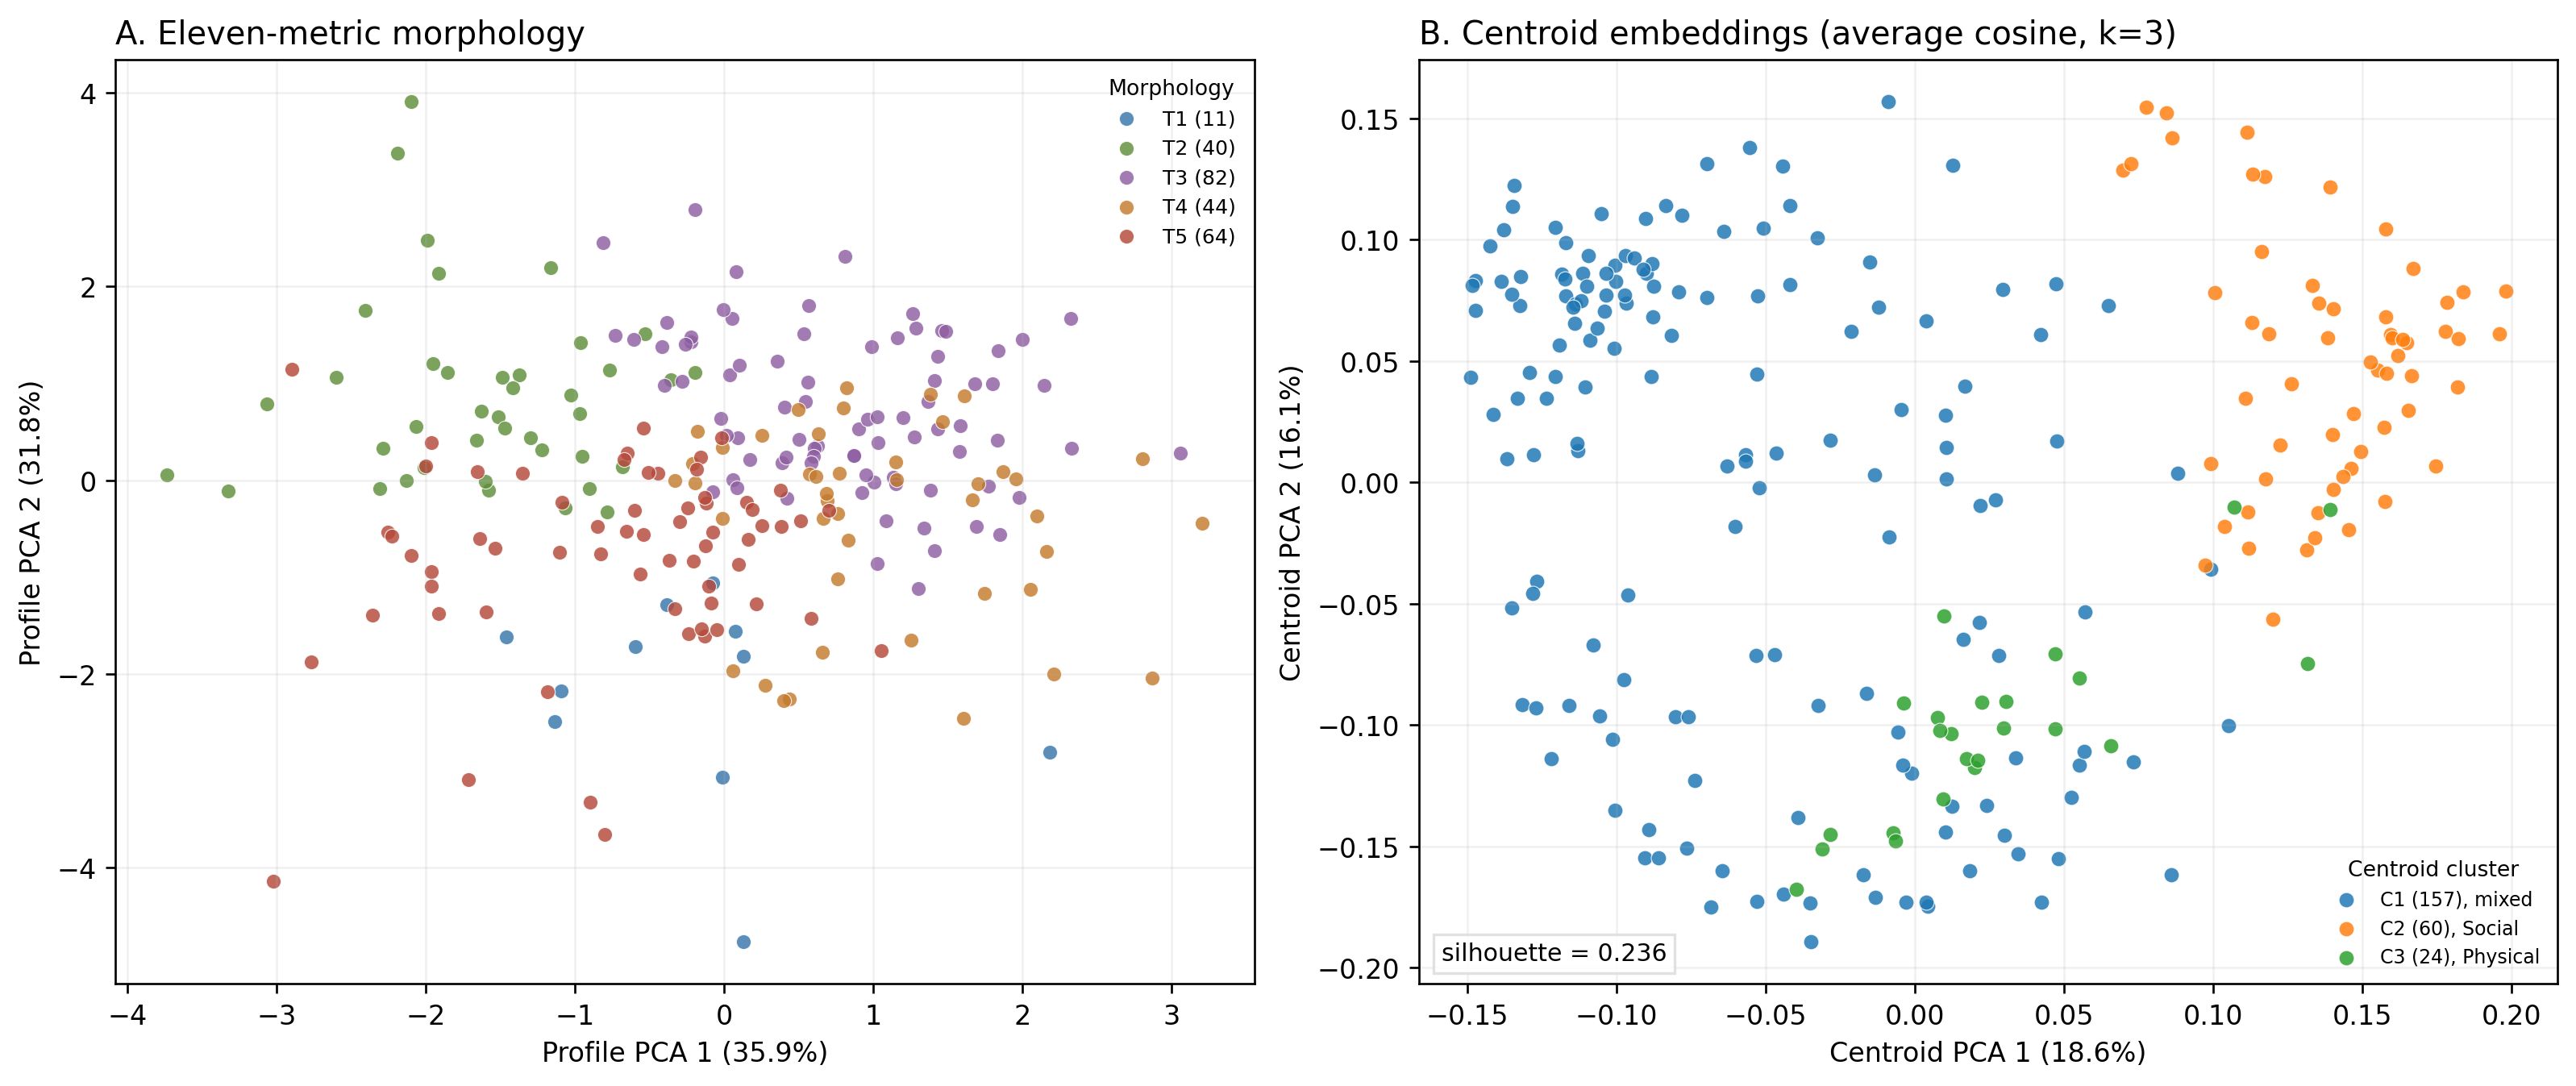
\includegraphics[width=\textwidth]{figures/fig_09_centroid_embedding_clustering_sensitivity.png}
\end{figure}

\section{Temporal-Trajectory and Hybrid Clustering Sensitivity}

Two further sensitivity checks ask whether the weak morphology typology changes when the representation is altered. The temporal-trajectory check clusters subfields by change in the eight windowed structural metrics across the five thesis windows. Because one subfield lacks a completed 2000--2004 window, this check uses 240 complete trajectories. Four representations were tested: first--last change vectors, linear slope vectors, full window-by-metric trajectories, and a dynamic summary combining changes, slopes, volatility, and centroid-path movement.

The best balanced temporal solution uses average-link hierarchical clustering on correlation distances between the eight-metric slope vectors, with \(k=4\), silhouette \(=0.396\), and cluster sizes \(93\), \(58\), \(54\), and \(35\). Its mean subsample ARI is \(0.725\), so this dynamic partition is more stable than the full-period morphology typology. It is not, however, the same object: agreement with the Chapter~9 morphology typology is low (AMI \(=0.048\)), and agreement with OpenAlex domains is also low (AMI \(=0.093\)). The groups are better read as dynamic tendencies: one cluster becomes more compact and locally denser; another expands in centroid and nearest-neighbor distance while hubness falls; a third loosens local neighborhoods while local unevenness declines; and a smaller group gains dimensionality and hub concentration.

The hybrid check combines semantic location with morphology. Two families were tested: concatenating balanced morphology profiles with reduced centroid principal components, and weighted distance matrices \(D_{\mathrm{hybrid}}=\alpha D_{\mathrm{centroid}}+(1-\alpha)D_{\mathrm{morphology}}\) for \(\alpha\in\{0.25,0.50,0.75\}\). The best balanced hybrid solution uses spectral clustering on the \(\alpha=0.75\) hybrid distance matrix, with \(k=3\), silhouette \(=0.247\), and cluster sizes \(91\), \(77\), and \(73\). It is highly stable under subsampling (mean ARI \(=0.951\)), but it aligns much more with centroid/domain structure than with morphology: AMI is \(0.591\) against OpenAlex domains, \(0.505\) against centroid clusters, and only \(0.092\) against the morphology typology. The hybrid result therefore confirms that semantic location dominates once it receives substantial weight.

These checks add nuance rather than a replacement typology. Temporal trajectories are useful for Chapter~7-style questions about how morphology changes; hybrid clusters are useful for showing how quickly semantic location reconstructs broad disciplinary structure. The Chapter~9 typology remains the appropriate summary for full-period morphology profiles.

\begin{figure}[H]
\centering
\caption[Temporal and hybrid clustering sensitivity]{Temporal and hybrid clustering sensitivity. Panel A projects the selected temporal slope-vector solution into PCA space and colors subfields by dynamic cluster. Panel B shows the OpenAlex domain composition of the selected hybrid centroid--morphology solution. The temporal projection is for visualization only; clustering uses standardized slope vectors. The hybrid solution uses a weighted distance matrix, not PCA or UMAP coordinates.}
\label{fig:temporal_hybrid_clustering_sensitivity}
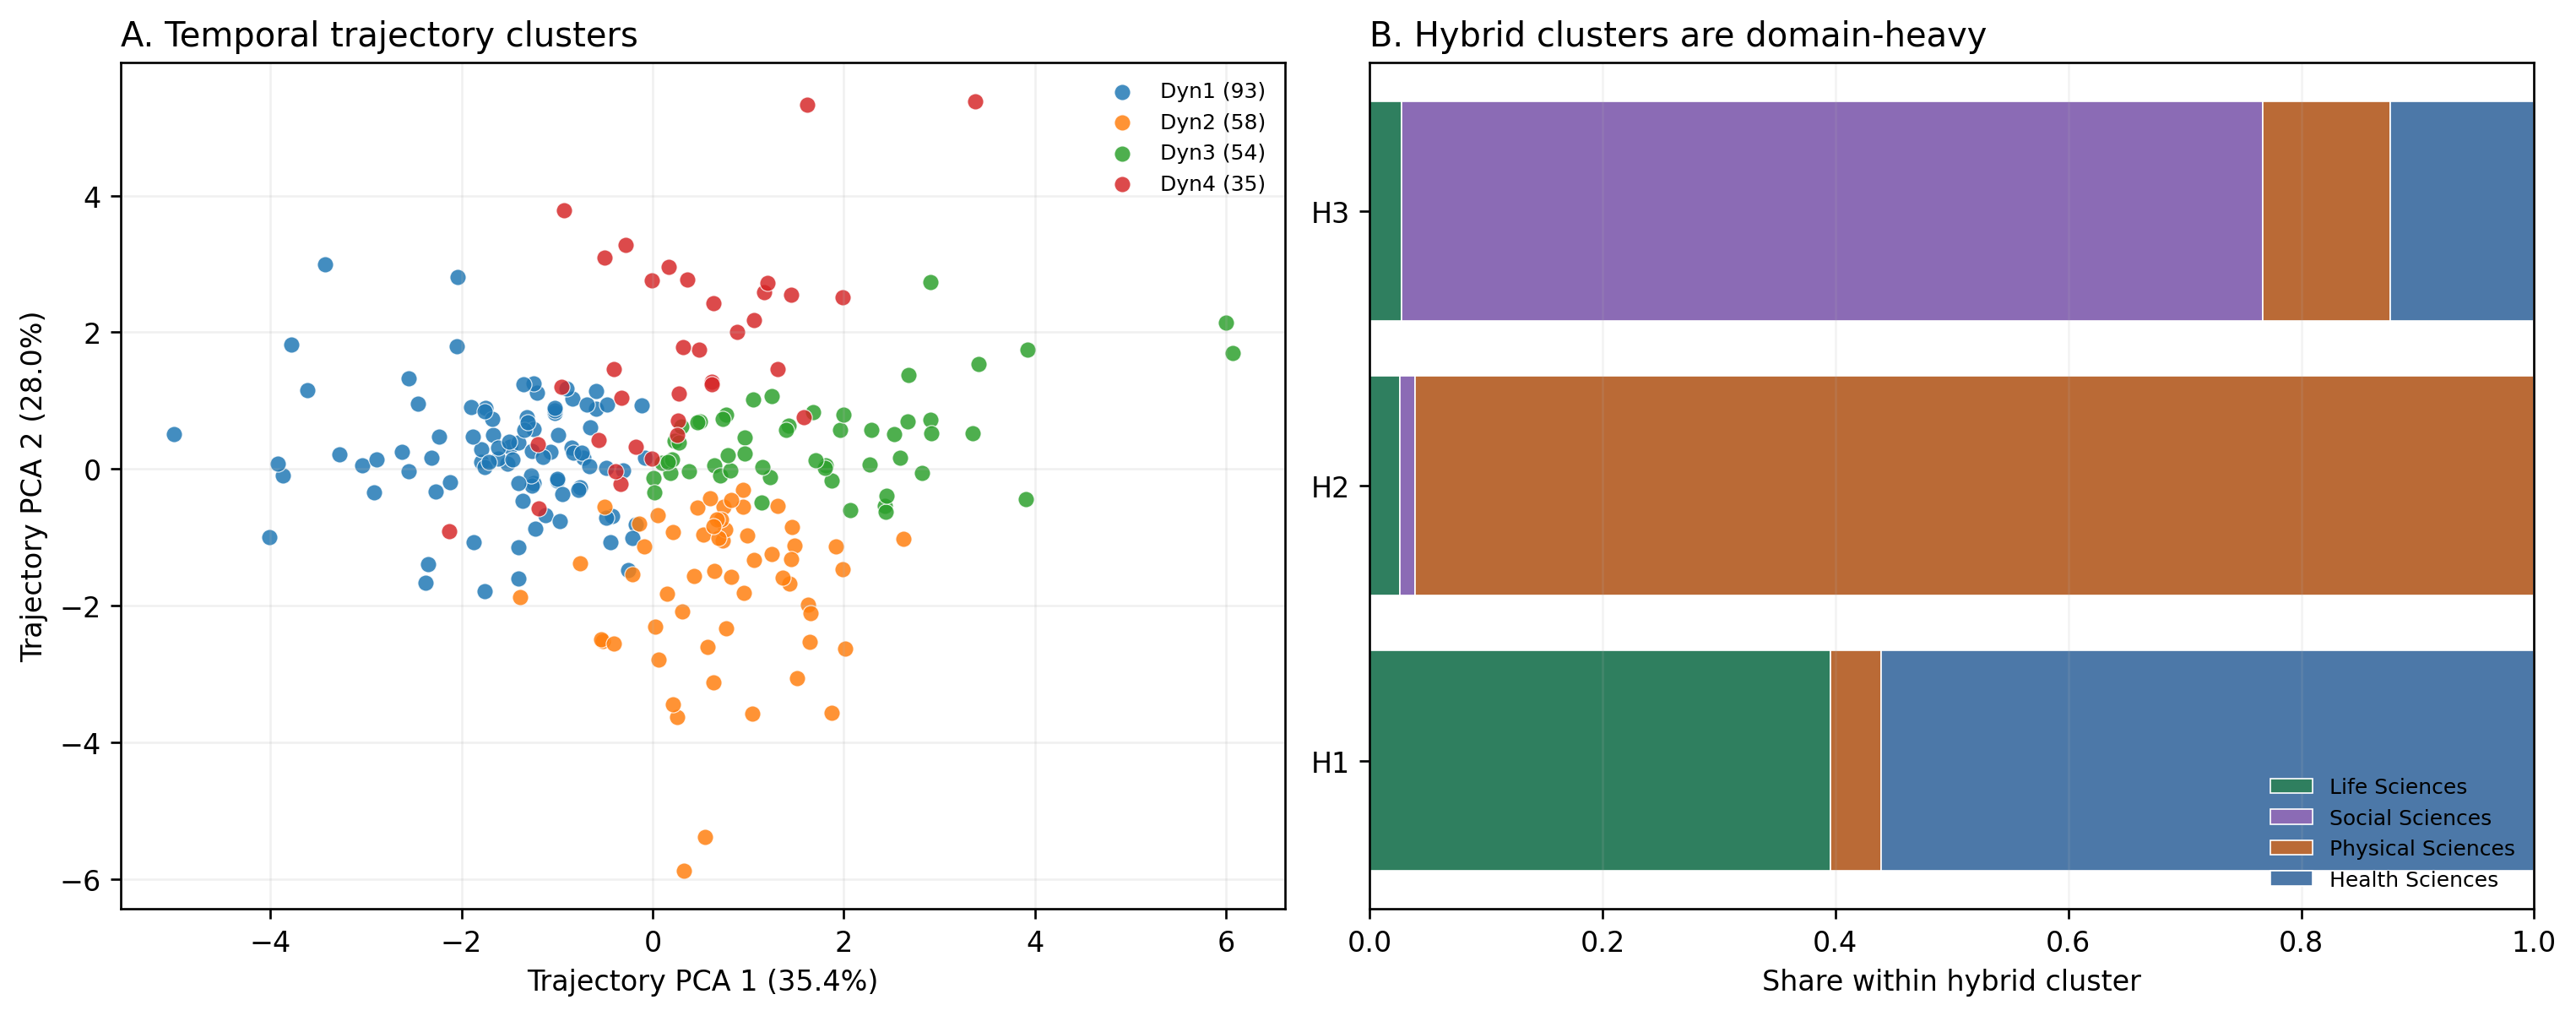
\includegraphics[width=\textwidth]{figures/fig_c_temporal_hybrid_clustering_sensitivity.png}
\end{figure}

% TODO: Include Spearman and Pearson metric correlation heatmaps.
% TODO: Include metric distribution histograms across all subfields.
% TODO: Include granular smooth density UMAP subfield panels for inspection.


\chapter{Illustrative UMAP Atlas of Selected Subfields}
% Appendix D: Illustrative UMAP Atlas of Selected Subfields

This appendix provides an illustrative atlas of selected subfield-level UMAP projections.
The panels are not used to compute morphology metrics, assign clusters, measure distances,
or support quantitative claims. They are included as visual diagnostics to make selected
paper-cloud morphologies interpretable at the document-cloud level. All quantitative claims
in the thesis remain based on metrics computed in the original SPECTER2 embedding space.
Because each panel is a separate subfield-specific UMAP projection, axes, distances, shapes,
and density scales should not be compared across subfields.

The atlas maps were generated separately for each selected subfield from the row-aligned
SPECTER2 analysis matrix, using main-analysis records from 2000--2024 and at most
10,000 papers per subfield. The per-subfield UMAP routine used cosine distance with
\texttt{n\_neighbors = 30}, \texttt{min\_dist = 0.05}, \texttt{random\_state = 42}, and
\texttt{low\_memory = true}. The density panel is a \texttt{smooth\_hist} rendering:
a 150-by-150 two-dimensional histogram over the displayed UMAP coordinates, smoothed
with a Gaussian filter of \(\sigma = 3.0\), clipped at the 99th percentile of positive
density values, and drawn with \texttt{viridis}. The atlas-generation script reads the
stored SPECTER2 matrix directly; no additional vector-normalization step is exposed in
that plotting routine. These settings are reported for reproducibility only, and the
resulting coordinates are not used for quantitative measurement.

The selected cases are not the visually prettiest maps in isolation. They are chosen because
they connect to recurring empirical themes in the thesis: atypical profiles, dispersed
physical-science structure, compact or separated local organization, computer-science novelty,
and broad material-science morphology. These figures are intended as visual companions to the
metric-based interpretation in Chapters 6--9. The six cases cover an atypical social-science
profile, a dispersed physical-science cloud, a compact life-science structure with a separated
component, two computer-science novelty cases, and a broad material-science morphology.

% Figure 1: Human Factors and Ergonomics
\begin{figure}[p]
    \centering
    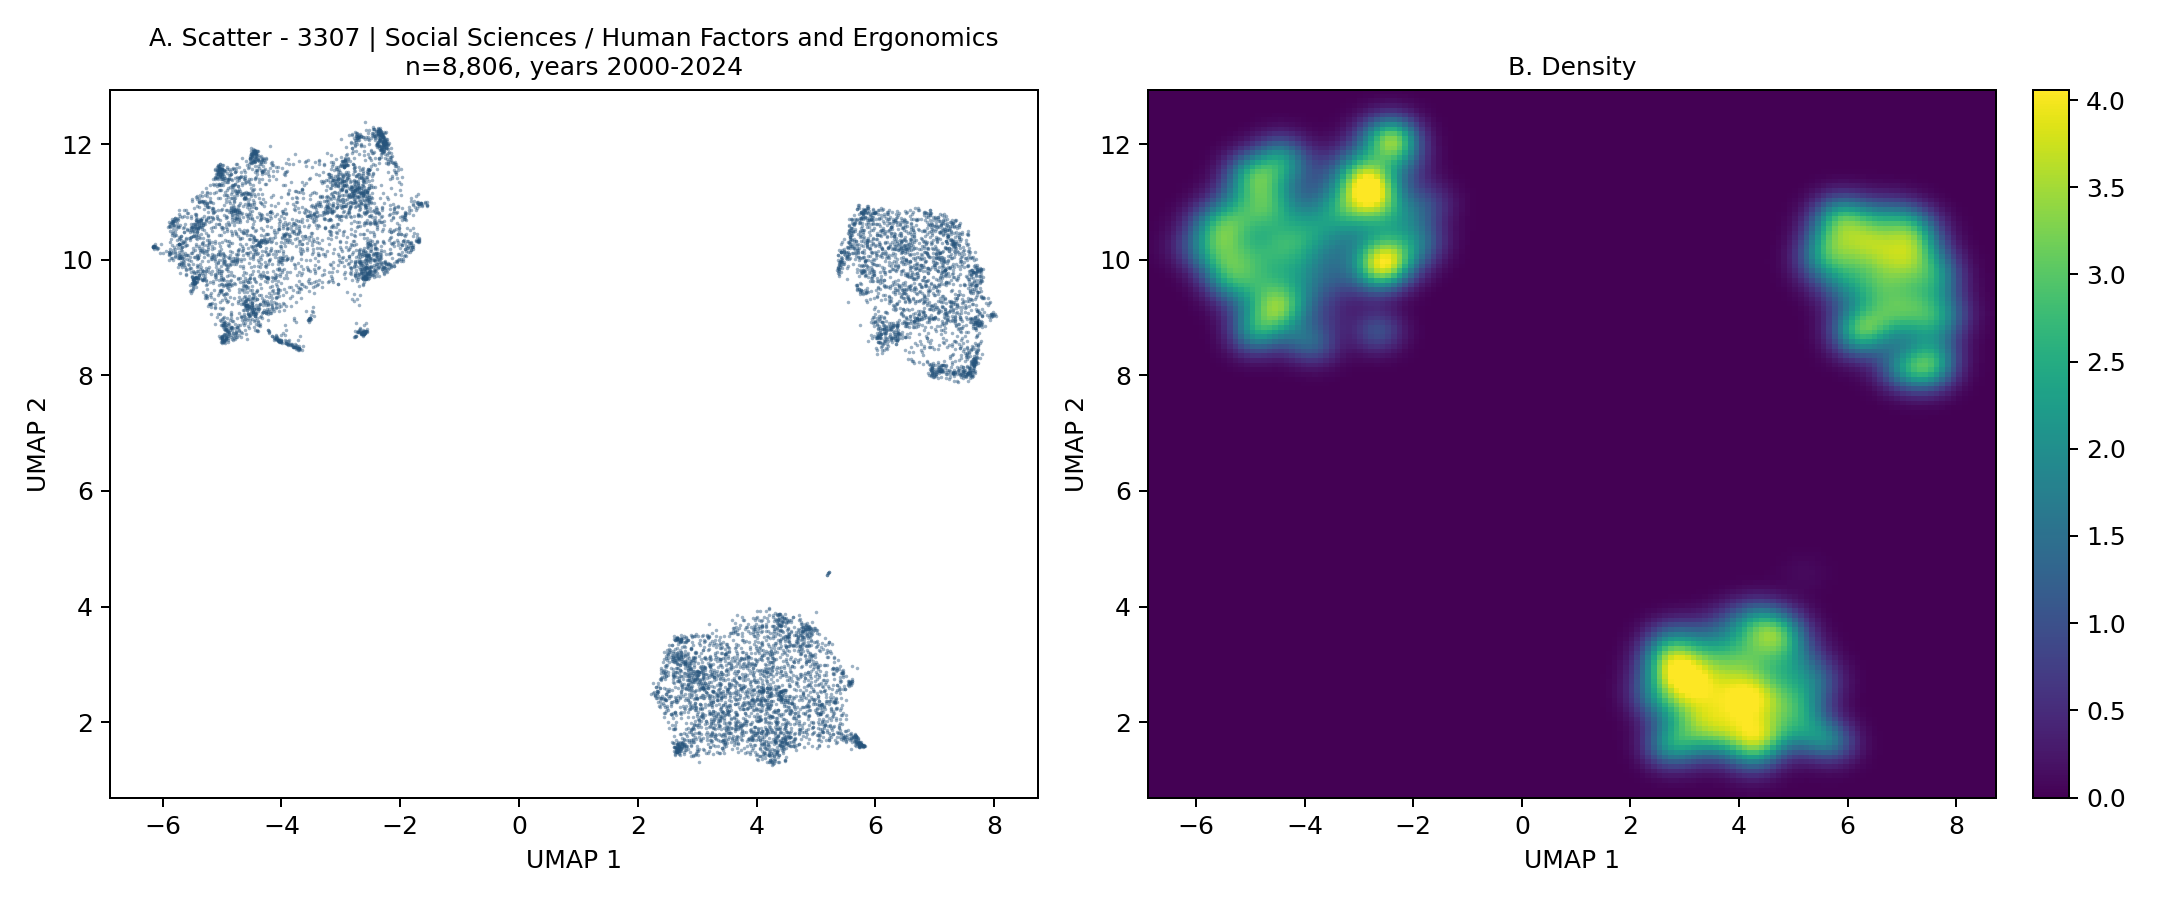
\includegraphics[width=\textwidth]{figures/umap_atlas/fig_d_umap_human_factors_ergonomics.png}
    \caption[Illustrative UMAP atlas: Human Factors and Ergonomics]{%
        Illustrative UMAP atlas: Human Factors and Ergonomics.
        The separated paper-cloud components make this case visually useful for interpreting
        the atypical profile behavior discussed in the thesis. The projection is illustrative
        only; quantitative metrics are computed in the original SPECTER2 space.}
    \label{fig:umap_atlas_human_factors}
\end{figure}

% Figure 2: Nuclear and High Energy Physics
\begin{figure}[p]
    \centering
    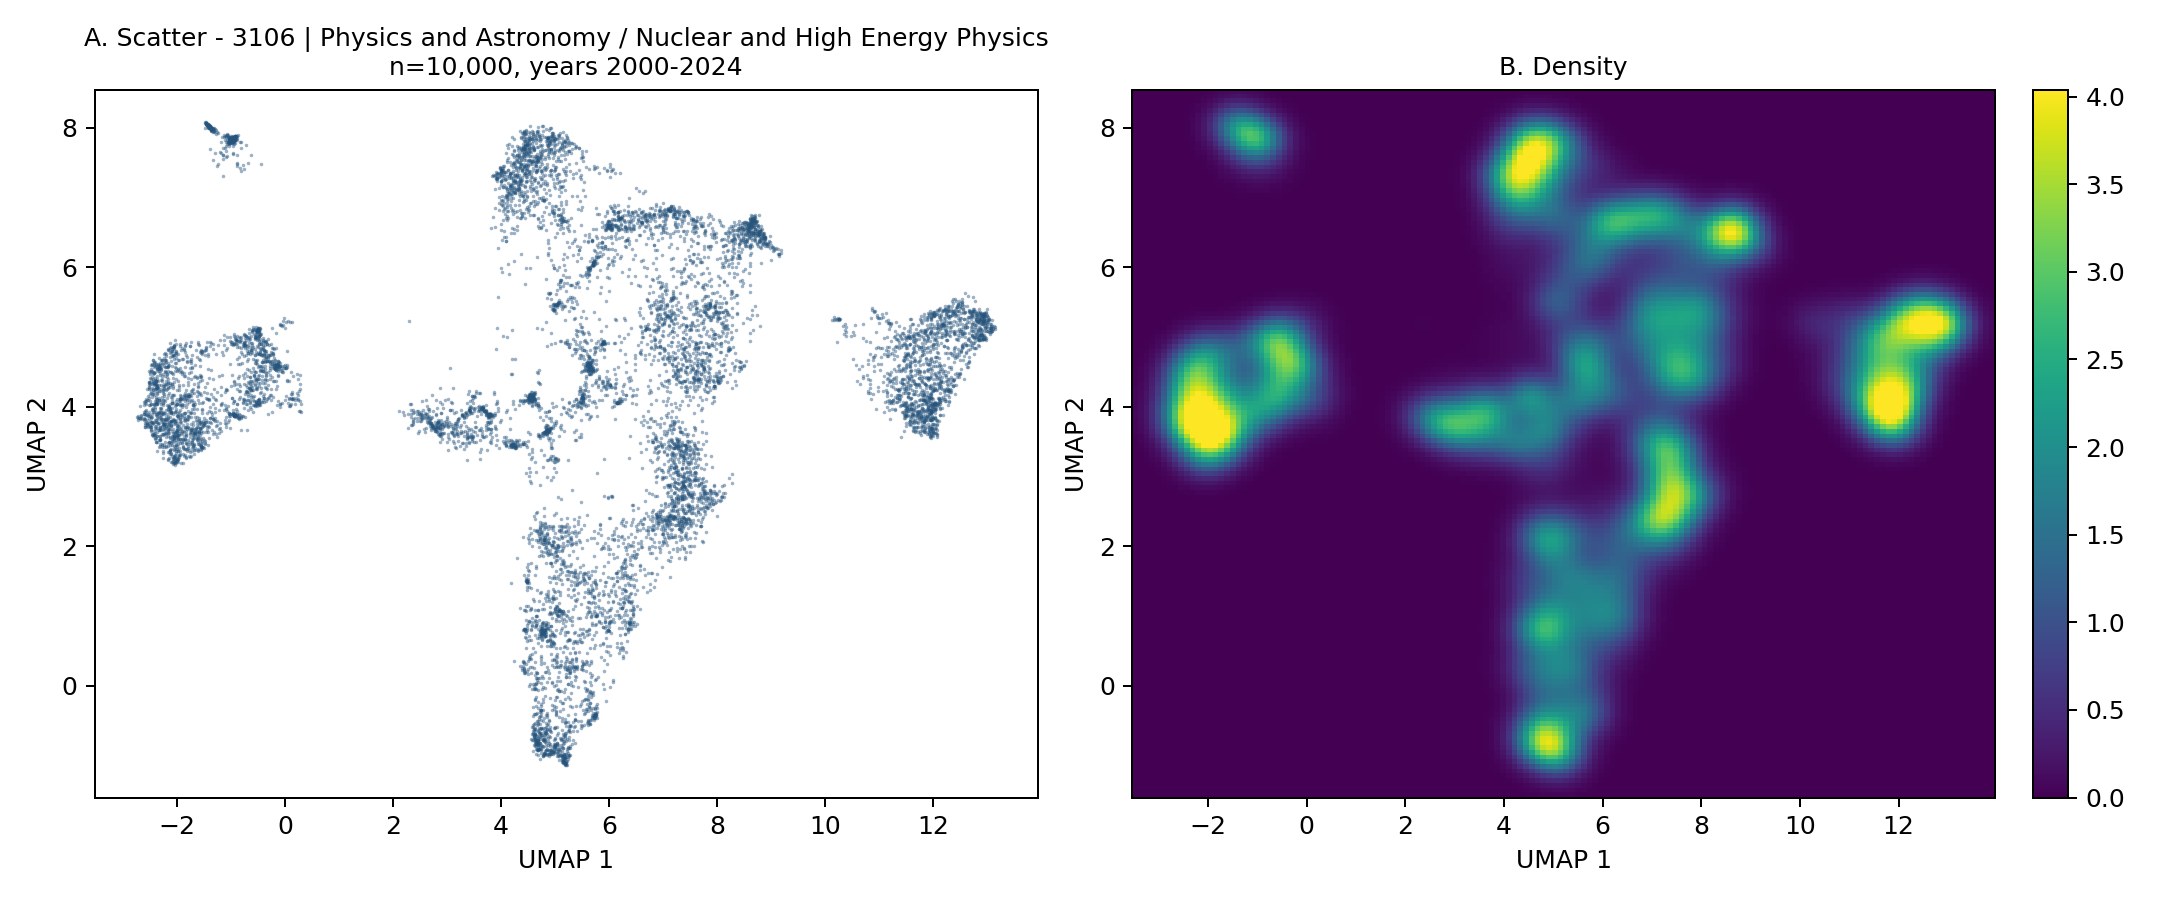
\includegraphics[width=\textwidth]{figures/umap_atlas/fig_d_umap_nuclear_high_energy_physics.png}
    \caption[Illustrative UMAP atlas: Nuclear and High Energy Physics]{%
        Illustrative UMAP atlas: Nuclear and High Energy Physics.
        The fragmented visual structure provides an example of a dispersed physical-science
        paper cloud. UMAP is used only as a subfield-level visualization and not as a
        measurement space.}
    \label{fig:umap_atlas_nuclear_physics}
\end{figure}

% Figure 3: Applied Microbiology and Biotechnology
\begin{figure}[p]
    \centering
    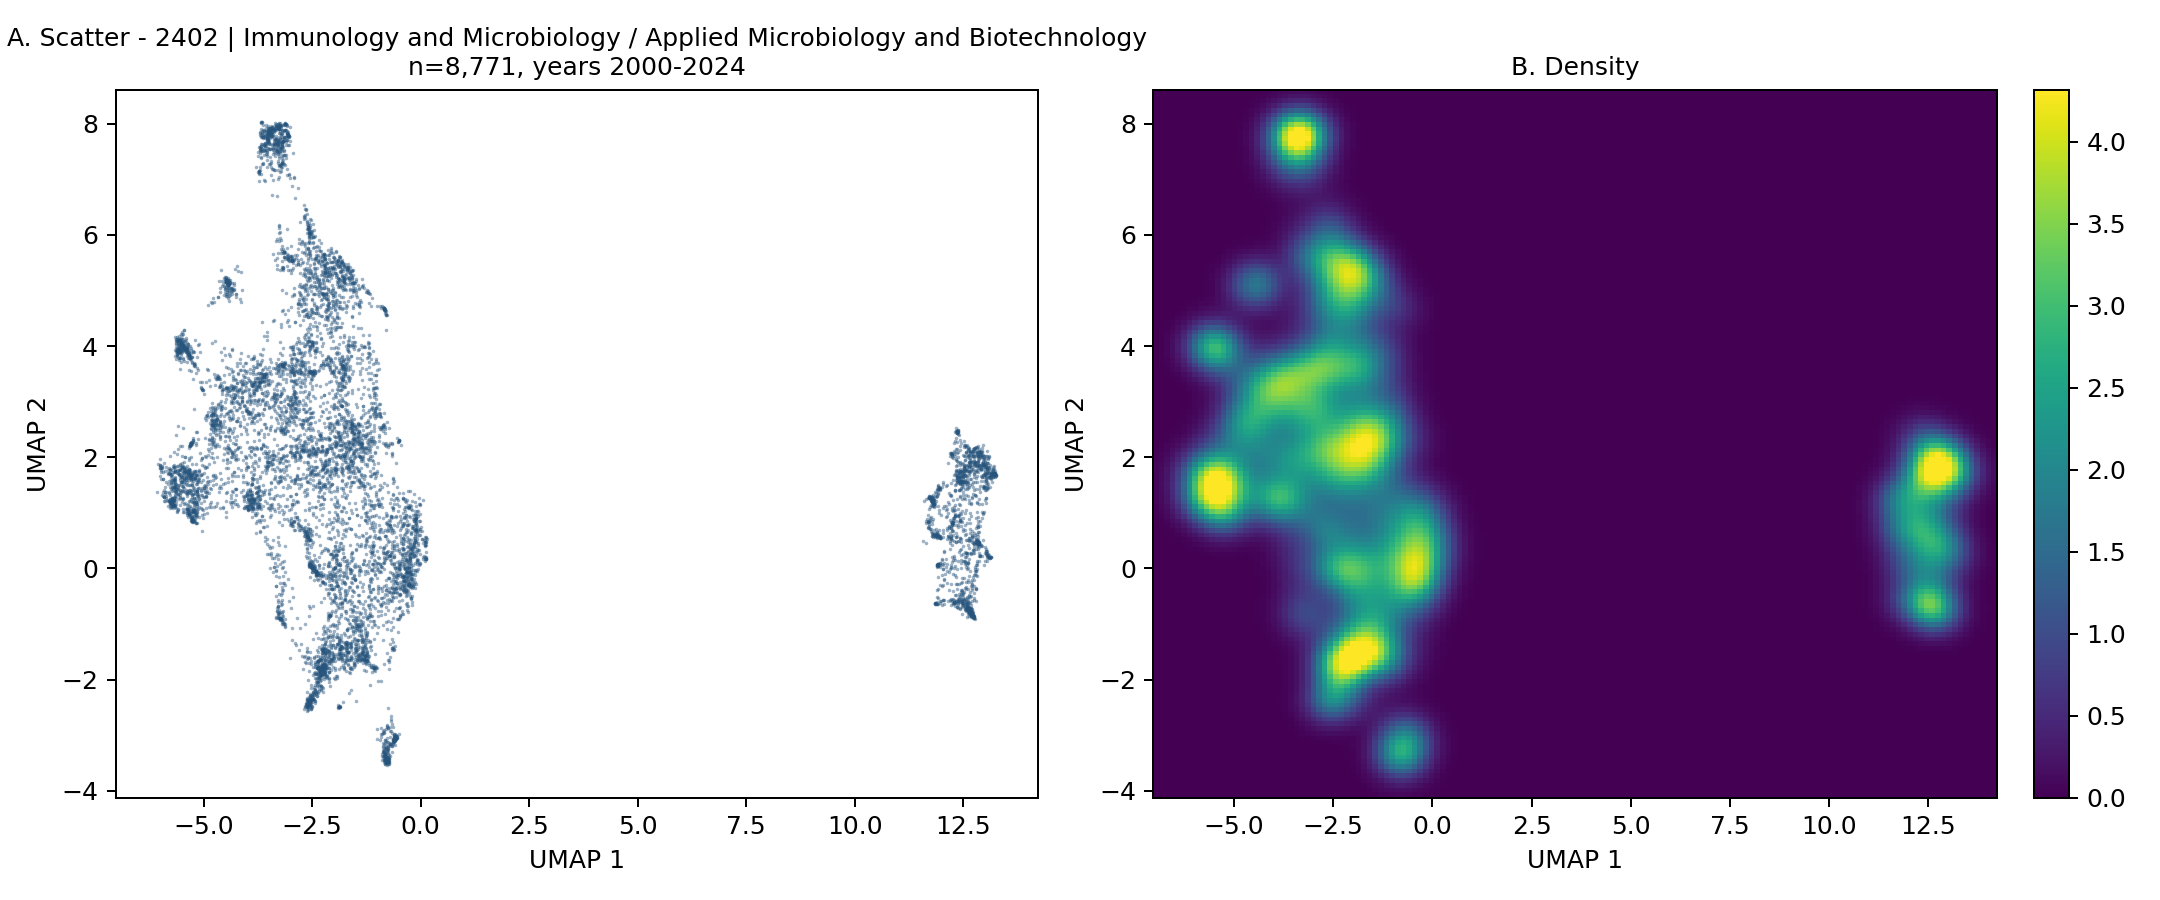
\includegraphics[width=\textwidth]{figures/umap_atlas/fig_d_umap_applied_microbiology_biotechnology.png}
    \caption[Illustrative UMAP atlas: Applied Microbiology and Biotechnology]{%
        Illustrative UMAP atlas: Applied Microbiology and Biotechnology.
        The map illustrates a dense main region together with a separated component,
        making the case useful for visualizing local organization beyond a single centroid.
        The projection is illustrative only.}
    \label{fig:umap_atlas_applied_microbiology}
\end{figure}

% Figure 4: Computer Vision and Pattern Recognition
\begin{figure}[p]
    \centering
    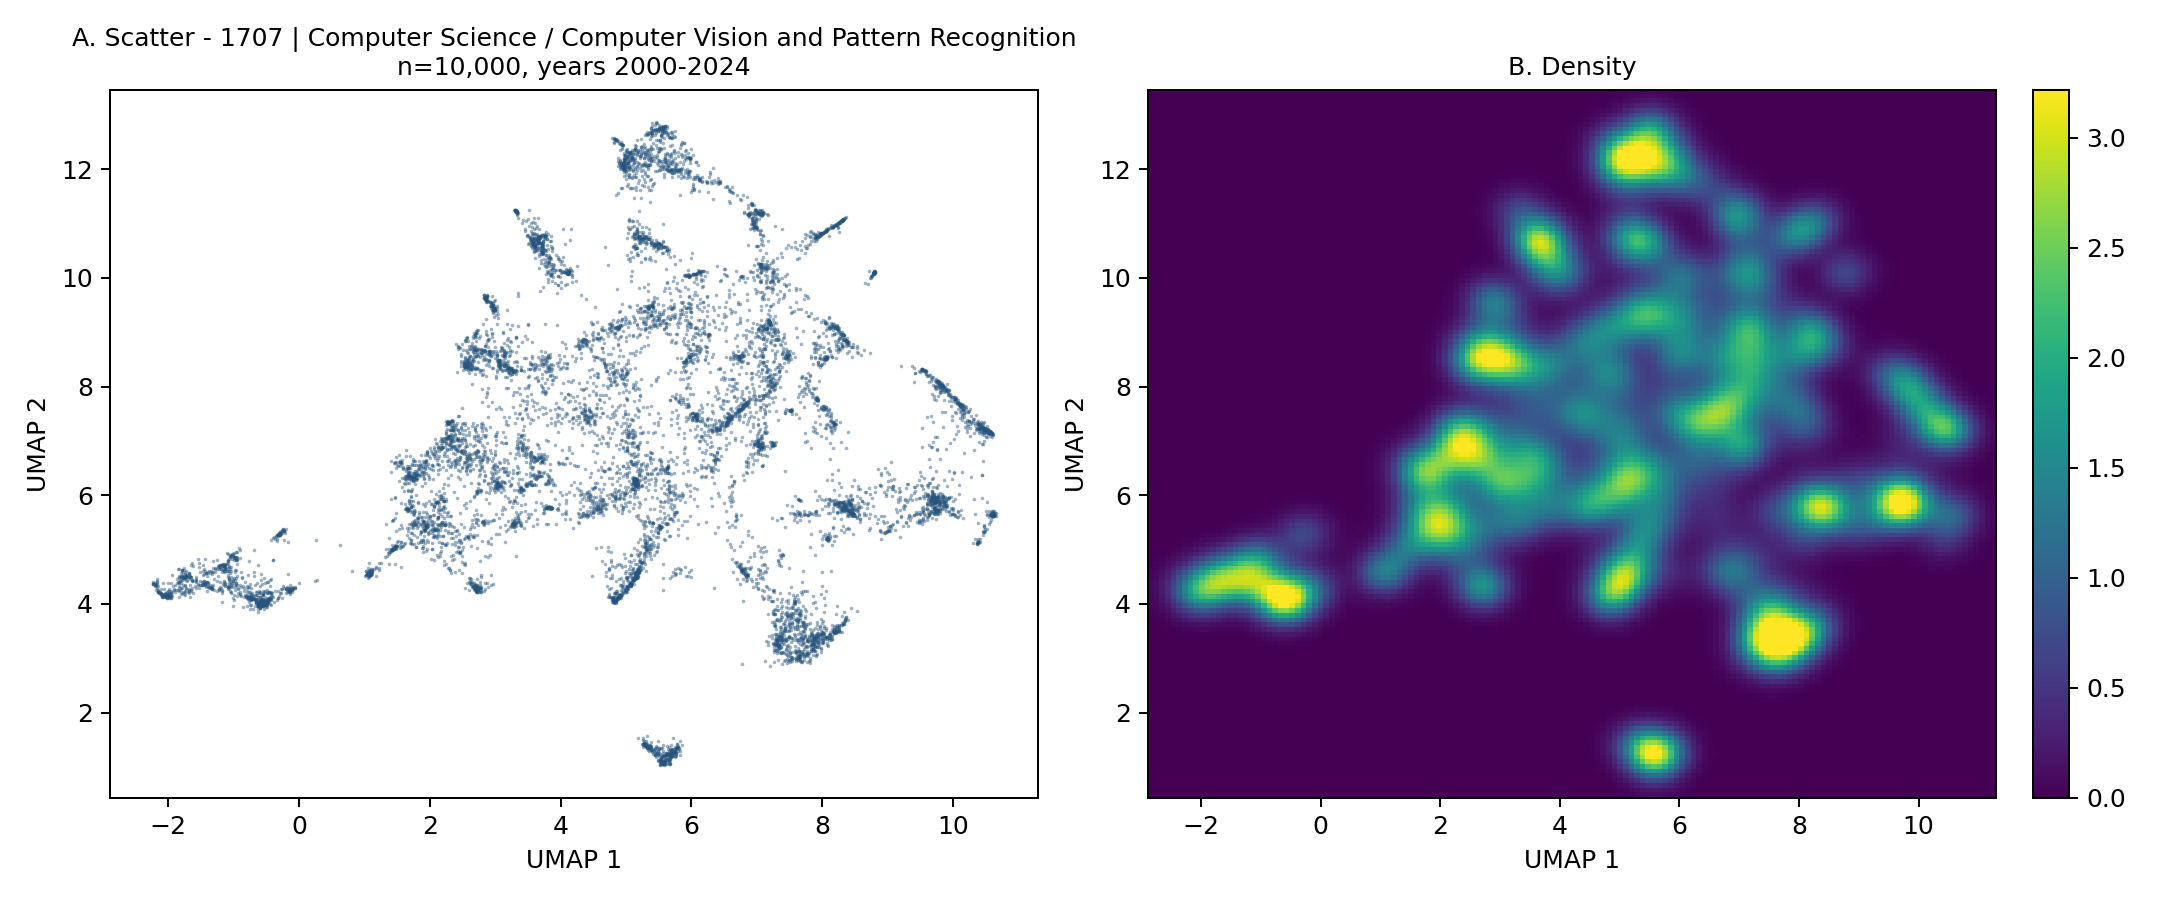
\includegraphics[width=\textwidth]{figures/umap_atlas/fig_d_umap_computer_vision_pattern_recognition.png}
    \caption[Illustrative UMAP atlas: Computer Vision and Pattern Recognition]{%
        Illustrative UMAP atlas: Computer Vision and Pattern Recognition.
        The panel provides a visually rich Computer Science example connected to the thesis
        discussion of novelty and movement. The projection is not used to define clusters
        or distances.}
    \label{fig:umap_atlas_computer_vision}
\end{figure}

% Figure 5: Signal Processing
\begin{figure}[p]
    \centering
    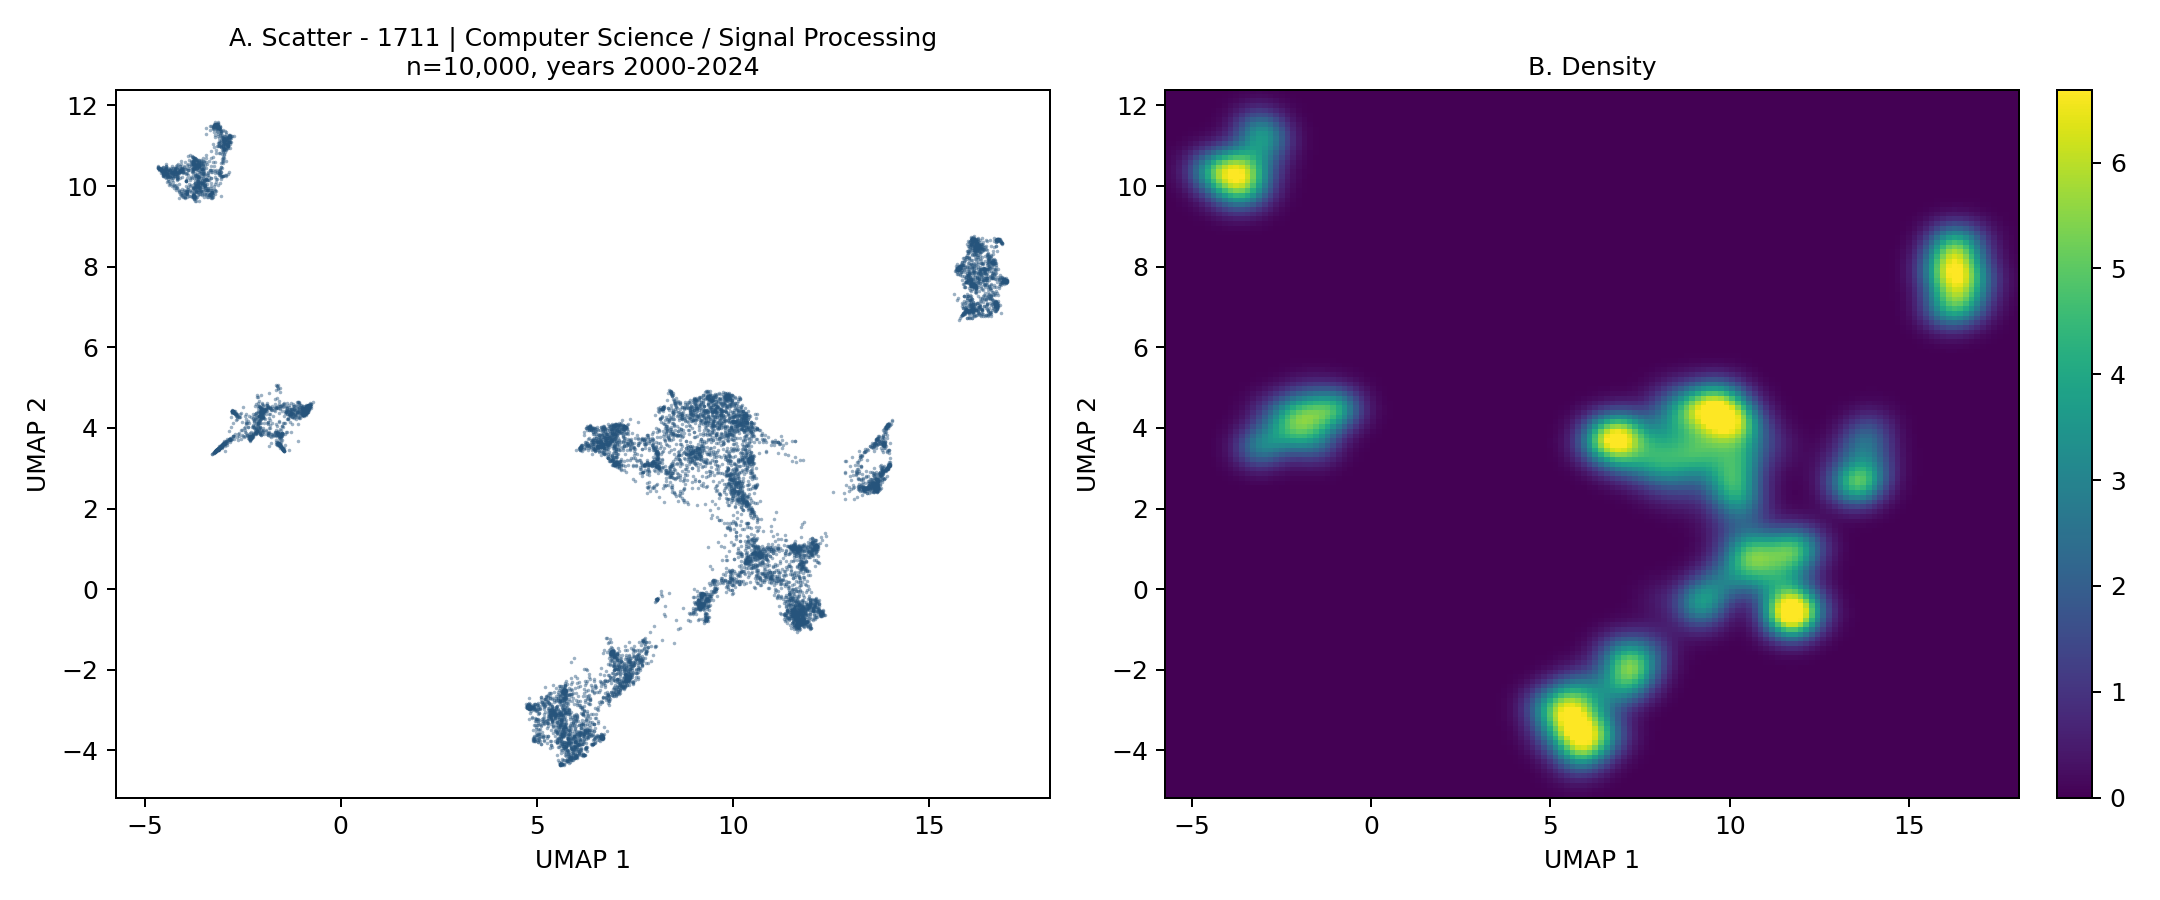
\includegraphics[width=\textwidth]{figures/umap_atlas/fig_d_umap_signal_processing.png}
    \caption[Illustrative UMAP atlas: Signal Processing]{%
        Illustrative UMAP atlas: Signal Processing.
        The separated components make this a useful visual companion to the temporal and
        novelty-oriented Computer Science cases. The projection is illustrative only and
        should not be compared geometrically with other panels.}
    \label{fig:umap_atlas_signal_processing}
\end{figure}

% Figure 6: General Materials Science
\begin{figure}[p]
    \centering
    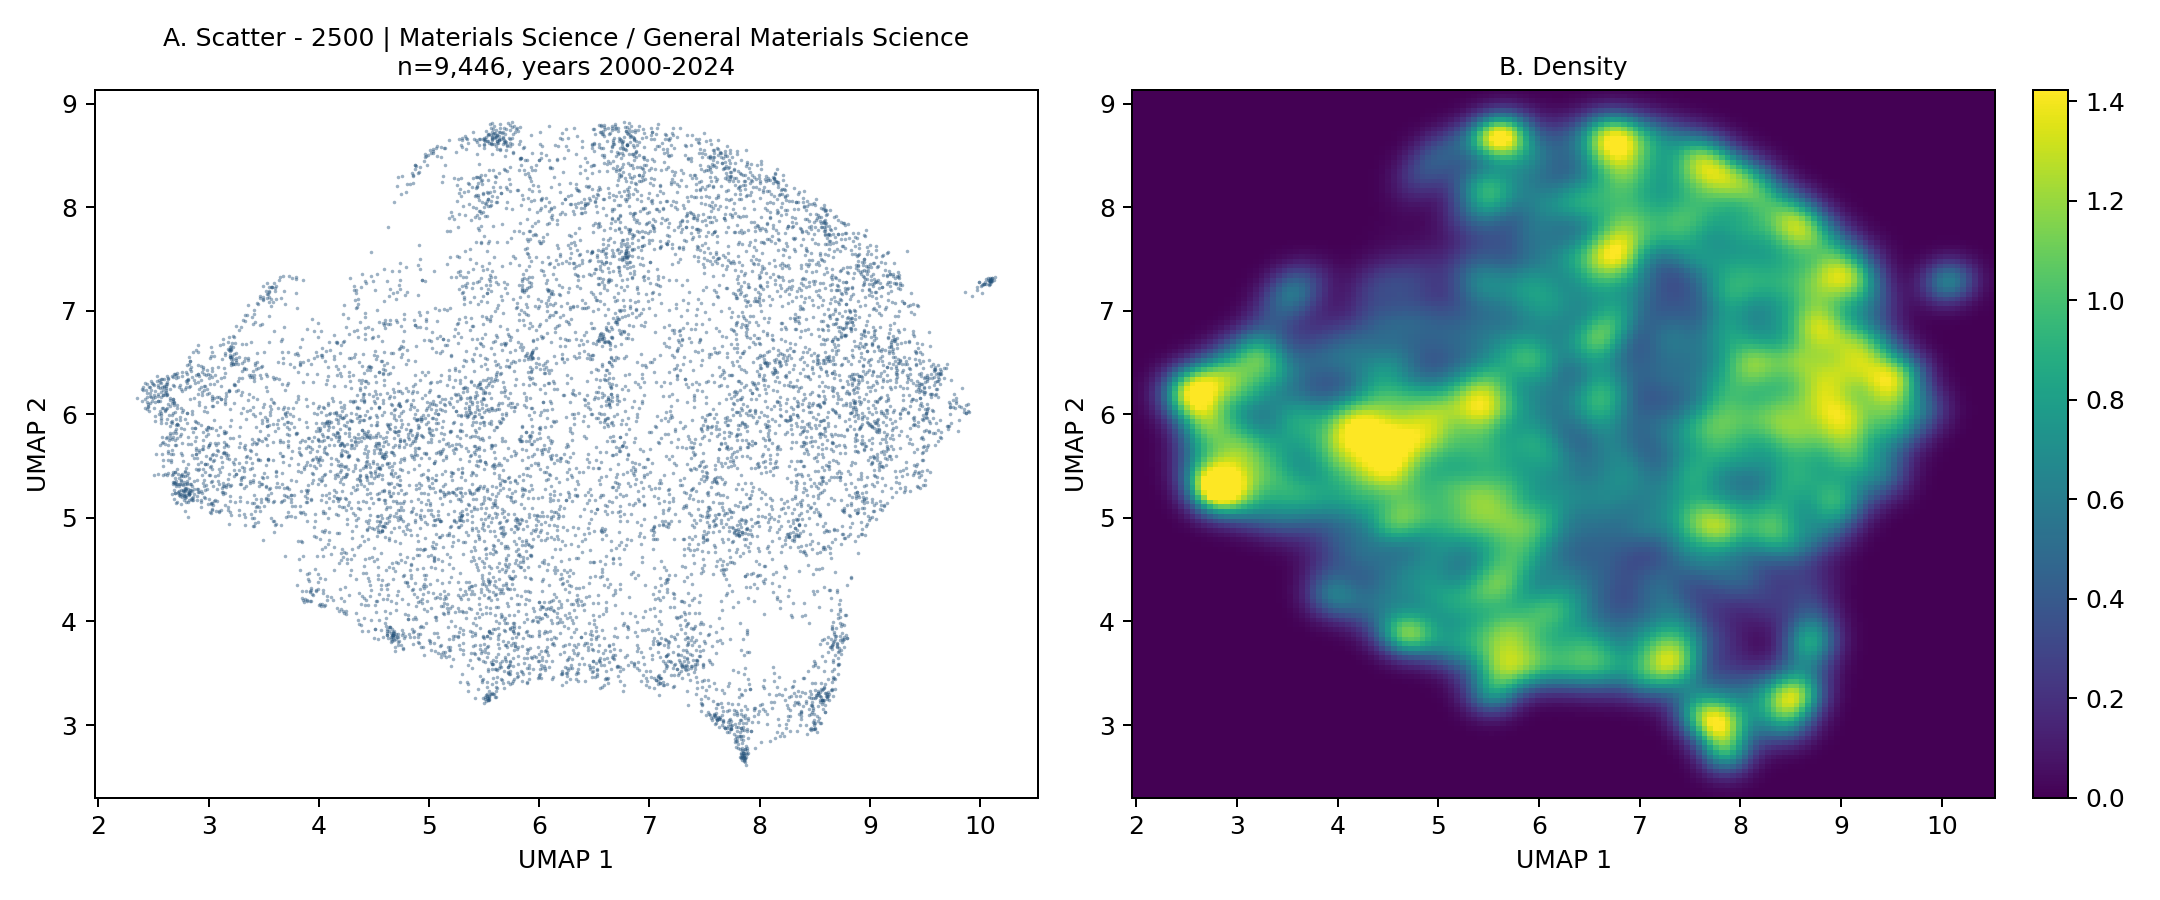
\includegraphics[width=\textwidth]{figures/umap_atlas/fig_d_umap_general_materials_science.png}
    \caption[Illustrative UMAP atlas: General Materials Science]{%
        Illustrative UMAP atlas: General Materials Science.
        The broad continuous cloud provides a contrast to the more fragmented examples in the
        atlas and illustrates why morphology is not reducible to a single centroid. Quantitative
        interpretation remains based on original-space metrics.}
    \label{fig:umap_atlas_general_materials}
\end{figure}


\end{document}
